%
%
%
%%%%%%%%%%%%%%%%%%%%%%%%%%%%%%%%%%%%%%%%%%%%%%%%%%%%%%%%%%%%%%%%%%%
\chapter{Hybrid Grid Solver for Turbulent Viscous Flow}
\label{flow_model.chap}
\heada{Hybrid Grid Solver for Turbulent Viscous Flow}
\setcounter{footnote}{0}
%%%%%%%%%%%%%%%%%%%%%%%%%%%%%%%%%%%%%%%%%%%%%%%%%%%%%%%%%%%%%%%%%%%
%
%
%
 This chapter presents a method for solving steady and unsteady, compressible,
 turbulent viscous flows for 2D and 3D turbomachinery blades.
 The flow model is based on the Favre-averaged Navier-Stokes equations,
 together with a one equation turbulence model.
 The space discretisation uses a node-centered finite volume scheme
 on unstructured mixed element grids, consisting
 of triangles and quadrilaterals in 2D, and of tetrahedra, pyramids, 
 triangular prisms and hexahedra in 3D. 
 The important features of the present approach are the 
 discretisation of the domain via a single, unified {\em edge-data structure}
 for mixed-element meshes and the use of a Laplacian weight
 which results in nearest neighbour stencils.
 The Laplacian weight is evaluated using an approximation of the
 Galerkin finite element method.
 In order to allow a straightforward implementation of fluid-structure
 coupling, the numerical solution is based on the Arbitrary
 Lagrangian-Eulerian method in which the grid points may be moved
 in an arbitrary but specified way.
 The pseudo time integration for steady-state problems is obtained using a
 preconditioned agglomeration multigrid method designed for highly
 anisotropic unstructured hybrid grids.
 In order to use the same preconditioned multigrid
 algorthim employed in the steady-state cases,
 a dual time-stepping technique is used for unsteady computations.
%
%
%
%
%
%
%
\section{Introduction}
\label{intro_nonlinear.sec}
\headb{Nonlinear Navier-Stokes solver}{Introduction}
%
 Over the last decade, significant advances have been made
 in the area of turbulent-viscous simulations using unstructured
 grids.
 However, compared with their structured counterparts,
 standard unstructured grid solvers have lower computational
 efficiency in terms of speed and storage.
 Unstructured grids often use tetrahedral elements only,
 an approach which often leads to numerical problems when the region to be
 discretised has a preferred direction such as the boundary layer for a
 high-Reynolds number flow. However, there are no fundamental difficulties in 
 extending tetrahedral meshes to include further element types such as triangular prisms, 
 pentahedra and hexahedra.  
 Although both the discretisation of the computational domain and the flow solver
 will become more complex,  such a mixed-element approach will offer
 a better, more efficient approximation than using tetrahedral elements only.
 For instance, hexahedral elements will handle boundary layer flows much better
 than tetrahedral elements because they can be made very slender without
 creating excessively small internal angles. 
 In order to handle mixed-element meshes, the spatial discretisation
 of the governing equations needs to be formulated in such a way
 that the numerical algorithms can be applied in a uniform way to all
 element types.
 A relatively simple way of achieving such consistent numerical treatment
 is to employ an edge-based data structure, which can be obtained
 from either a finite volume (FV) or a finite element (FE) formulation
 if the mesh consists of tetrehedral elements only. In this particular case, 
 all nodes are connected directly without any internal diagonals.
 However, quadrilaterals in 2D and hexahedrals in 3D have not only
 edges but also diagonal links. Therefore, to create an edge-based
 data structure from mixed meshes, one cannot use a FE technique
 because of the non-zero shape function contributions from the
 diagonally-opposed nodes for which there are no direct edges.
 Consequently, we will use a FV technique to obtain an edge-based
 data structure from mixed element meshes but, as reported by
 Barth \citeyear{Barth:4}, Parthasarathy et al. \citeyear{Kallinderis:2},
 Mavriplis \& Venkatakrishnan \citeyear{Mavriplis:3}
 for unstructured meshes of tetrahedra, 
 the discretisation of the viscous terms, remains a major problem. 
 The FV edge-based data structure is usually obtained by
 discretising the viscous terms in two sequential  loops, the so-called
 two-loop approach. The first loop is used to construct the gradients
 at all points, and the second one forms the second derivatives from
 the computed gradient information.
 Using such a technique, 
 the viscous fluxes are treated in an analogous manner to
 the inviscid ones and no extra storage is required.
 However, this strategy, used by several authors
 (see Peraire et al. \citeyearNP{Peiro:2}, Vahdati \& Imregun \citeyearNP{Mehdi:3})
 has at least three serious drawbacks.
 First, the {\em odd-even decoupling} can destabilize
 the numerical scheme in regions where the viscous effects are
 important, e.g. the boundary layer.
 Second, for a 1D mesh of spacing $h$, the scheme will reduce to a second
 difference on a stencil of $2h$, a feature which will lower numerical
 accuracy.  Since packing enough points into the viscous layer
 is one of the main difficulties associated with viscous flow
 computations, a scheme that operates on every other point is highly
 undesirable.
 The third problem is the difficulty of implementing a viscous Jacobian which
 becomes important if an implicit time integration scheme is employed.

 An alternative approach, based on Galerkin
 finite element (GFE) approximation where velocity
 and temperature are made dependent variables,  is the derivation of the six node-pair
 coefficients for the Hessian matrix (Mavriplis \citeyearNP{Mavriplis:4},
 Selmin \& Formaggia \citeyearNP{Formaggia}).
 Each coefficient  is associated with  two nodes only, hence the term "node-pair GFE". 
 As mentioned earlier, such a formulation is not edge-based for non-tetrehedral meshes because 
 of the possible diagonal links between the nodes of a hexahedral element.
 On the other hand, the final discrete viscous
 terms of such a GFE formulation form a nearest neighbour stencil.
 Therefore, using the  Hessian node-pair
 coefficients, six second derivatives can be calculated for each node.
 Since the viscous terms can be expressed as a summation of the product
 of the node-pair coefficients and the unknowns,
 the construction of a viscous Jacobian becomes straightforward by explicit
 differentiation. Furthermore, the odd-even decoupling is avoided and the accuracy is improved.
 Unfortunately, this approach needs additional storage for the six node-pair
 coefficients and its applicability is restricted to triangular/tetrahedral
 elements if an edge-based data structure needs be employed.

 In summary, when dealing with mixed-element meshes, FV formulations can
 yield edge-based data structures but viscous flux discretisation
 remains problematic. On the other hand, GFE formulations are more
 efficient but the edge-based data structure cannot be preserved for non tetrahedral elements.  
 Therefore, the discretisation of the viscous fluxes
 can be improved by combining  the
 storage efficiency of the two-loop FV approach  with the
 numerical efficiency of the node-pair GFE method in an edge-based FV framework.

%
%
\section{Favre Averaged Navier-Stokes Equations}
\label{mathematical_model.sec}
\headb{Nonlinear Navier-Stokes solver}{Flow equations}
%
 The system of Navier-Stokes equations constitute the most complete
 description of viscous, heat-conducting flows and represents the highest
 level of approximation for continuous fluids.
 However, from the point of view of computational fluid dynamics,
 the vast majority of flow situations occurring in engineering
 applications enter into a particular form of instability, called
 {\em turbulence}.
 This occurs in most flow situations when the inertial forces
 exceed the viscous forces by more than four orders of magnitude
 (the ratio of these two forces is called {\em Reynolds number}).
 This form of instability can be represented by statistical
 fluctuations of the flow quantities around mean or averaged values.
 Moreover, the space scale of these fluctuations is so small that their
 direct calculation is beyond the reach of computational capabilities
 for engineering applications.

 Therefore, time-averaged Navier-Stokes equations need to be considered
 in most situations.
 In the case of compressible flow equations, this averaging
 is called Favre averaging (Wilcox \citeyearNP{Wilcox}).
 Because of the non-linearity of the Navier-Stokes equations, this
 procedure generates additional unknowns which will be solved using a
 suitable turbulence model. 
 In this work, the Spalart Allmaras \citeyear{Spalart:1} one equation
 turbulence model has been used (Appendix \ref{turbulence.chap}).
%
%
%
%
\subsection{Mean flow equations}
\label{conservative_formulation.subsec}
%
%
 The unsteady, compressible, Favre-averaged Navier-Stokes
 equations for a blade row in 3D can be cast in terms of
 absolute velocity $\vec{v}$ but solved in a relative non-Newtonian reference frame
 rotating along with the blade about the $x$ axis with angular velocity
 ${\bf \Omega}$ as shown in Fig. \ref{axis.fig}.
 This system of equations, written in a dimensionless, Arbitrary
 Lagrangian-Eulerian (ALE), integral conservative
 form (Donea et al. \citeyearNP{Donea}) for a control
 volume ${\cal V}\left(t\right)$ with boundary
 ${\cal S}\left(t\right)$
 in Cartesian coordinates $\vec{x} = \left(x, y, z\right)$,
 takes the form
%
\beq
  \fpdt{} \int_{{\cal V}\left(t\right)} {\bf U} d{\cal V} +
  \oint_{{\cal S}\left(t\right)} \left[
  \vec{{\bf F}} \left({\bf U}, \vec{u}\right) -
  \frac{1}{Re}\vec{{\bf G}} \left({\bf U}, \nabla {\bf U}\right) \right]
  \cdot\vec{n}\, d{\cal S} =
  \int_{{\cal V}\left(t\right)} {\bf S}\,d{\cal V}
  \label{conservative_formulation_nl.eq}
\eeq
%
%
\begin{figure}[ht]
  \centerline{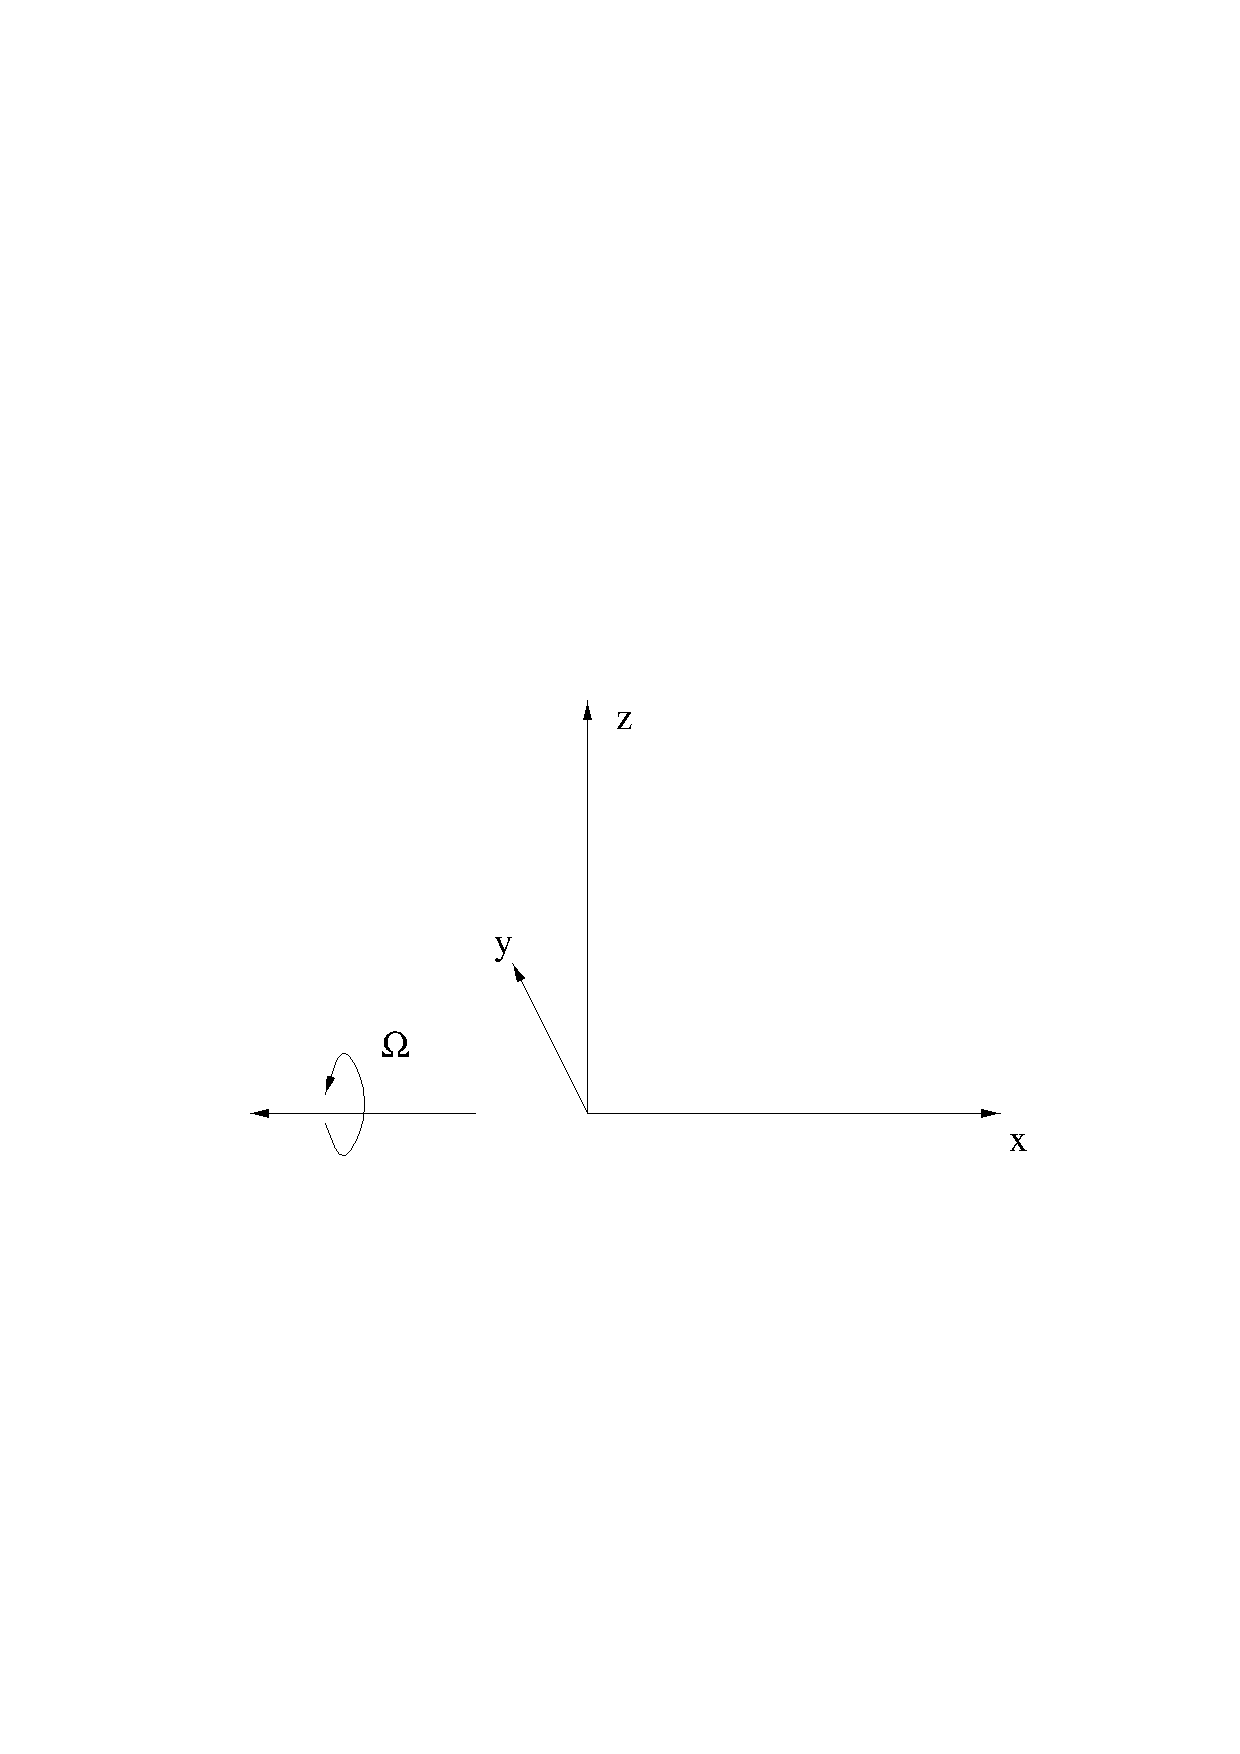
\includegraphics[width=60mm,clip=t]{CHAP_NONLIN/FIGURE/axis.pdf}}
  \caption{Direction of blade rotation}
  \label{axis.fig}
\end{figure}
%
 The viscous term $\vec{\bf G}$
 on the left-hand side of (\ref{conservative_formulation_nl.eq})
 is scaled by the reference Reynolds number so that flow variables are
 non-dimensionalised consistently. The dimensionless quantities are evaluated
 from their dimensional counterparts using the dimensional reference values
 reported in Appendix \ref{nondim.chap}.
 $\vec{n}$ represents the outward unit vector of the control volume boundary
 ${\cal S}\left(t\right)$. The vector $\vec{u}$, which represents the
 velocity in the relative frame of reference minus the velocity
 $\frac{d \vec{x}}{d t}$ of the boundary
 ${\cal S}\left(t\right)$, can be written as:
%
\beq
   \vec{u} = \vec{v} - \vec{\Omega} \times \vec{x} - \frac{d \vec{x}}{d t}
   \label{relative_velocity.eq}
\eeq
%
 where $\vec{\Omega} = \left(-\Omega,0,0\right)$. The sign of the angular velocity vector
 is determined by the assumption that the positive rotational speed is the
 one indicated in Fig. \ref{axis.fig}.
 The solution vector of conservative variables ${\bf U}$ is given by:
%
\beq
   {\bf U} = \left[
   \begin{array}{ccccc}
   \rho & \rho v\sm{1} & \rho v\sm{2} & \rho v\sm{3} & \rho E
   \end{array}
   \right]\se{T}
   \label{conservative_variables.eq}
\eeq
%
 The inviscid flux vector  $\vec{{\bf F}}\left({\bf U}, \vec{u}\right)$
 has the following components\footnote{${\bf U}u\sm{j}$ represents the $j$ component
 of the convective flux, while ${\bf F}{\scriptstyle p}\sm{j}$ represents the $j$ component
 of the pressure flux.}:
%
\beq
   {\bf F}\sm{j} &=& {\bf U}u\sm{j} + {\bf F}{\scriptstyle p}\sm{j}
   \label{nonlinear_inviscid_flux.eq}\\
   {\bf F}{\scriptstyle p}\sm{j} &=&
   \left[
   \begin{array}{ccccc}
   0 & p\delta\sm{1j} & p\delta\sm{2j} & p\delta\sm{3j} & v\sm{j} p
   \end{array}
   \right]\se{T}
   \label{nonlinear_pressure_flux.eq}
\eeq
%
 where $\delta\sm{ij}$ represents the Kronecker delta function.
 The static pressure $p$ and the total energy $E$ are related, in
 a non-dimensional fashion, to the density
 $\rho$, absolute velocity $\vec{v}$ and total enthalpy $H$
 by the following two equations which assume perfect gas with a constant
 ratio $\gamma$ of specific heat.

%
\beq
  p = \left(\gamma - 1\right) \rho \left[E - \frac{\left|\vec{v}\right|\se{2}}{2}\right],
  \ \ \ \ \ \
  H = E + \frac{p}{\rho}
 \label{pressure_energy_relations.eq}
\eeq
%
 Following the approach of Sbardella \& Imregun \citeyear{Luca:7,Luca:11},
 the viscous part of the governing equations is split into
 two distinct components, namely:

%
\beq
 \vec{\bf G} = \vec{\bf G}{\scriptstyle l} + \vec{\bf G}{\scriptstyle m}
 \label{viscous_terms.eq}
\eeq
%
 where

%
\beq
 \vec{\bf G}{\scriptstyle l} = \left[
 \begin{array}{c}
  0 \\ \mu \nabl v\sm{1} \\
       \mu \nabl v\sm{2} \\
       \mu \nabl v\sm{3} \\
       \mu\sum\sm{j=1}\se{3} v\sm{j}\nabl v\sm{j}
      + \frac{\gamma}{\gamma\!-\!1}
       \left(\frac{\mu\sm{l}}{Pr\sm{l}}\!+\!\frac{\mu\sm{t}}{Pr\sm{t}}\right) \nabl T
 \end{array} \right]
 \label{mean_flow_laplacian.eq}
\eeq
%
 $T=p/\rho$ is the non-dimensional static temperature of the fluid.
 The $j$-component of the second term on the left-hand side of
 (\ref{viscous_terms.eq}) is:

%
\beq
 {\bf G}{\scriptstyle m}\sm{j} = \left[
 \begin{array}{c}
  0 \\ \mu \fpd{v\sm{j}}{x\sm{1}} +
       \left(\lambda\nabl\cdot\vec{v}\right)\delta\sm{1j}\\
       \mu \fpd{v\sm{j}}{x\sm{2}} +
       \left(\lambda\nabl\cdot\vec{v}\right)\delta\sm{2j}\\
       \mu \fpd{v\sm{j}}{x\sm{3}} +
       \left(\lambda\nabl\cdot\vec{v}\right)\delta\sm{3j}\\
       \mu\left(\vec{v}\cdot\nabl v\sm{j}\right) +
       \lambda v\sm{j}\left(\nabl\cdot\vec{v}\right)
 \end{array} \right]
 \label{mean_flow_mixed.eq}
\eeq
%
 In (\ref{mean_flow_laplacian.eq}) and (\ref{mean_flow_mixed.eq}),
 $\mu$ represents the total dynamic viscosity of the fluid and is given
 by the summation of the laminar (physical) dynamic viscosity $\mu\sm{l}$
 and the turbulent dynamic viscosity $\mu\sm{t}$.
 The value of $\lambda$ is given by the
 Stokes relation $\lambda = -\frac{2}{3} \mu$
 which is valid for the majority of the flow situations with the exception
 of very high temperature or pressure ranges.
 It is easily seen that the
 component $\vec{\bf G}\sm{l}$ in (\ref{mean_flow_laplacian.eq})
 includes  the Laplacian operators of the three velocity components and
 temperature only.
 The second component, $\vec{\bf G}\sm{m}$, contains the mixed derivative terms,
 while the vector of source terms ${\bf S}$ on the right-hand side of
 (\ref{conservative_formulation_nl.eq}) takes into accounts for the blade
 rotation

%
\beq
  {\bf S} = \left[
   \begin{array}{ccccc}
    0 & 0 & \rho \Omega v\sm{3} & -\rho \Omega v\sm{2} & 0
   \end{array}
   \right]\se{T}
   \label{source_term.eq}
\eeq
%
 The derivation of the constitutive relations of viscous flows is discussed
 in detail by Schlichting \citeyear{Schlichting} and White \citeyear{White:1}.

%
\subsection{Boundary conditions}
\label{boundary_conditions_nonlinear.subsec}
%
%
%
 For convection dominated phenomena, such as those described by the 
 compressible Navier-Stokes equations, the formulation of correct boundary
 conditions is extremely important and its impact on the numerical scheme
 is often dominating.
 The reason for this strong influence can be traced back to the physical nature of
 the convection propagation phenomena (Hirsh \citeyearNP{Hirsch:1}).
 If all the variables were known at a boundary from the knowledge of the
 physical input, there would be no difficulty; however this is generally not the
 case with hyperbolic systems of partial differential equations.
 The number of physical
 variables that can be freely imposed at a boundary is dependent on the propagation
 properties of the system and, in particular, on the information propagated from
 the boundary towards the inside of the flow region. These are known as
 {\em physical boundary conditions}. The remaing variables will depend on the
 details of the flow and are, therefore, part of the solution. However
 from a numerical point of view, information about all variables
 is required  at the boundary. This additional information gives rise to
 {\em numerical boundary conditions} (Hirsch \citeyearNP{Hirsch:1}).
 
 The presence of viscosity and heat conduction
 transforms the conservation laws of momentum and energy into second-order
 partial differential equations.
 The system of Navier Stokes equations is therefore an hybrid system consisting of
 parabolic momentum and energy equations and of a hyperbolic continuity equation.
 A direct consequence is the need for a greater number
 of physical boundary conditions when dealing with viscous flows instead of
 inviscid flows.
%
%
\paragraph{Flow-tangency.}
%
 Also known as the inviscid wall condition, this boundary condition at the solid walls
 is expressed by the requirement that there is no flow through the surface
 of the moving wall. Only one physical boundary condition can be imposed
 at this boundary because only the forward travelling acoustic wave is entering
 the domain. Mathematically, this condition is expressed by the vanishing of the
 velocity normal to the wall.

%
\beq
  \vec{u}\cdot\vec{n} = 0
  \label{flow_tangency1.eq}
\eeq
%
 Expressed in a {\em week sense}, i.e. through the fluxes, (\ref{flow_tangency1.eq})
 becomes:

%
\beq
 \oint\sm{wall}\vec{\bf F}d{\cal S} =
 \oint\sm{wall}\vec{\bf F}{\scriptstyle p}d{\cal S} =
 \left[
 \begin{array}{c}
 0 \\ p\ n\sm{1} d{\cal S}\\
      p\ n\sm{2} d{\cal S}\\
      p\ n\sm{3} d{\cal S}\\
      p\ \left(\vec{\Omega}\times\vec{x}+\frac{d \vec{x}}{d t}\right)\cdot\vec{n}d{\cal S}
 \end{array}
 \right]
  \label{flow_tangency2.eq}
\eeq
%
\paragraph{No-slip condition.}
%
%
 The no-slip condition at the solid walls is expressed by the requirement that the
 fluid velocity relative to the moving wall must be zero.
 Mathematically this can be expressed as:

%
\beq
  \vec{u} = \vec{v} - \vec{\Omega}\times\vec{x} - \frac{d \vec{x}}{d t} = 0
  \label{no_slip1.eq}
\eeq
%
 In addition to (\ref{no_slip1.eq}), an additional information is required
 due to the presence of the second derivative terms in the Navier-Stokes
 equations\footnote{The no-slip condition is valid for viscous flow only.}.
 Here this additional information is for an adiabatic wall

%
\beq
  \vec{n}\cdot\nabl T = 0
  \label{no_slip2.eq}
\eeq
%
%
\paragraph{Inflow and outflow boundaries.} 
%
 The quasi-3D non-reflecting boundary
 conditions developed by Saxer \& Giles \citeyear{Giles:7} are used
 for steady-state computations.
 These boundary conditions are obtained from a Fourier mode analysis
 of the linearised Euler equations at the far-field boundaries.
 Implemented in a turbomachinery environment, the approach assumes
 that the solution at the boundary is circumferentially decomposed into Fourier modes,
 the $0\se{th}$ mode corresponding to the averaged solution.
 The $0\se{th}$ mode is treated according to the standard 
 1D boundary condition (Thompson \citeyearNP{Thompson:1,Thompson:2})
 which allows the user to specify certain physical quantities at the boundaries.
 Such averaged quantities are:
%
\begin{itemize}
 \item
  {\bf Inflow:} stagnation temperature, stagnation pressure and flow angles.
 \item
  {\bf Outflow:} static pressure.
\end{itemize}
%
 The remaining part of the solution, represented by the sum of the harmonics,
 is treated according to the exact\footnote{The term exact refers to the
 solution of the linear problem. Since the linear problem is itself an approximation
 to the nonlinear one, there will be errors which are proportional to the square
 of the amplitude of the non-uniformities at the far-field boundaries.}
 2D theory of Giles \citeyear{Giles:5,Giles:6}.
 Since this method considers radial flow variations in the $0\se{th}$ mode only, it is
 called quasi-3D non-reflecting boundary conditions. In the absence of any radial
 variations, the boundary conditions are exact within
 the 2D linear theory.

 The  standard 1D characteristic boundary conditions of
 Thompson \citeyear{Thompson:1,Thompson:2} are used for 
 unsteady time-marching aerodynamics.
%
%
% 
\paragraph{Periodic boundaries.}
%
 Taking advantage of the edge-based data structure, the periodicity is handled in 
 a straightforward way as long as the points in the two periodic
 boundaries are located at same axial and radial coordinates.
%
\beq
  {\bf U}_{\theta_0 + \Delta \theta} = {\bf U}_{\theta_0}
\eeq
%

%
%
%
%
\section{Spatial Discretisation}
\label{space_discretisation_nl.sec}
\headb{Nonlinear Navier-Stokes solver}{Spatial discretisation}
%
 The development of a FV edge-based data structure
 for unstructured mixed-element meshes
 will now be described in detail.

%
\begin{figure}[ht]
\centerline{\includegraphics[width=80mm,clip=t]{CHAP_NONLIN/FIGURE/mixme.pdf}}
\caption{Control volume for node $I$ and metric vector
$\vec{\eta}\sm{IJs}$
 for edge $IJs$}
\label{median_dual.fig}
\end{figure}
%
 As shown for the 2D mesh of Fig. \ref{median_dual.fig},
 using a node-centered approach and choosing the median dual mesh as control
 volume\footnote{A discussion of different control volume definitions is
 given by Barth \& Jespersen 1989.},
 a FV discretisation of
 (\ref{conservative_formulation_nl.eq}), written
 in a semi-discrete form, is given by:

%
\beq
  \fpdt{\left({\cal V}\sm{I}{\bf U}\sm{I}\right)} &=& -\!
  \sum\sm{s=1}\se{m\sm{I}} \left[\left|\vec{\eta}\sm{IJs}\right|
  \left({\cal F}\sm{IJs}\!-\!{\cal G}\scriptstyle{m}\sm{IJs}\right)
  - \tau\sm{IJs} {\cal G}\scriptstyle{l}\sm{IJs}\right]
  + {\cal V}\sm{I}{\bf S}\sm{I}
  \label{semi_discrete_nl.eq}
\eeq
%
 As shown in Fig. \ref{median_dual.fig}, node $I$ is connected by edges to
 $m\sm{I}$ ($m\sm{I} = 6$ in Fig. \ref{median_dual.fig})
 nodes $J\sm{s}$, ${\cal V}\sm{I}$ representing the control volume
 associated with it.
 ${\cal F}$, ${\cal G}\scriptstyle{m}$ and ${\cal G}\scriptstyle{l}$
 correspond to the inviscid and viscous vectors $\vec{\bf F}$,
 $\vec{\bf G}\scriptstyle{m}$ and $\vec{\bf G}\scriptstyle{l}$.
 $\vec{\eta}\sm{IJs}$ is the metric vector associated with the
 surface area of edge $IJs$ while $\tau\sm{IJs}$ represents the Laplacian
 weight associated with the same edge.
 The summation in (\ref{semi_discrete_nl.eq}) has been obtained applying
 the Green's formula to the surface integral of (\ref{conservative_formulation_nl.eq})
 and choosing as path the median dual mesh (Barth \& Jespersen \citeyearNP{Barth:1},
 Barth \citeyearNP{Barth:2}).
 Of particular interest here is the use of the GFE node-pair formula
 for the Laplacian operator $\tau\sm{IJs}$ in order to construct
 an approximate version for the FV edge-data scheme
 (Sbardella \& Imregun \citeyearNP{Luca:7,Luca:11}).
%
%
%
%
%
\subsection{Inviscid discretisation}
\label{inviscid_disretisation.subsec}
%
 The discretisation of the inviscid flow terms in
 (\ref{semi_discrete_nl.eq}) is given by:

%
\beq
  \sum\sm{s=1}\se{m\sm{I}} \left|\vec{\eta}\sm{IJs}\right|
  {\cal F}\sm{IJs}
 \label{inviscid_contribution_nl.eq}
\eeq
%
 where ${\cal F}\sm{IJs}$ represents the inviscid flux function along edge
 $IJ\sm{s}$
 which is obtained using a central difference scheme with added
 matrix artificial dissipation. This artificial dissipation
 is a blend of second and fourth order differences. The fourth order
 terms ensure the stability of the scheme in smooth regions of the flow,
 while the second order terms are required to damp numerical oscillations
 in the vicinity of discontinuities.
 The inviscid flux function is expressed as:

%
\beq
  {\cal F}\sm{IJs} = \frac{\vec{\bf F}\sm{I}+\vec{\bf F}\sm{Js}}{2}
  \cdot\frac{\vec{\eta}\sm{IJs}}{\left|\vec{\eta}\sm{IJs}\right|}
  - {\cal D}\sm{IJs}
  \label{inviscid_flux_function_nl.eq}
\eeq
%
 where the artificial dissipation ${\cal D}\sm{IJs}$ along the edge is
 given by:

%
\beq
  {\cal D}\sm{IJs} = \frac{1}{2}
  \left|{\bf A}\sm{IJs}\right|
  \left[\psi\Delta{\bf U} - \epsilon\sm{4}\left(1-\psi\right)\Delta{\cal L}\left({\bf U}\right)\right]
  \label{artifical_diffusion_nl.eq}
\eeq
%
 Here $\Delta$ represents the difference operator along edge $IJs$

%
\beq
  \Delta\left(\cdot\right) = \left(\cdot\right)\sm{Js} -
\left(\cdot\right)\sm{I}
\label{difference_operator.eq}
\eeq
%
 $\left|{\bf A}\sm{IJs}\right|$ is the standard Roe matrix
 (Roe \citeyearNP{Roe:1})
 between the two stages ${\bf U}\sm{I}$ and ${\bf U}\sm{Js}$,
 $\epsilon\sm{4}\approx 1/16$ is the fourth order artificial dissipation
 coefficient. $\cal L\sm{I}\left({\bf U}\right)$ is a pseudo-Laplacian
 operator, at node $I$, given by:

%
\beq
  {\cal L}\sm{I}\left({\bf U}\right) =
  \left(\sum\sm{s=1}\se{m\sm{I}}
  \frac{{\bf U}\sm{Js}-{\bf U}\sm{I}}{s\sm{IJs}}\right)
  \left(\sum\sm{s=1}\se{m\sm{I}}
  \frac{1}{s\sm{IJs}}\right)\se{-1}
  \label{pseudo_lapl_nl.eq}
\eeq
%
 where

%
\beq
  s\sm{IJs} = \left|\vec{x}\sm{Js} - \vec{x}\sm{I}\right|
  \label{svalll.eq}
\eeq
%
 $\psi$ represents the limiter function which varies between
 0 and 1 and it is required in order to switch the scheme to first order
 ($\psi = 1$) in the vicinity of discontinuities (Jorgenson \&
 Turkel \citeyearNP{Turkel:2}).
%
%
\subsubsection{Evaluation of metric vector}
%
 The metric vector $\vec{\eta}\sm{IJs}$ is obtained
 via a summation of the two dual median lengths around the edges,
 multiplied by their normals. For example the metric vector of the edge
 connecting nodes $I$ and $Js$ is shown in Fig. \ref{median_dual.fig} for a
 2D mesh.
 Another way of calculating $\vec{\eta}\sm{IJs}$ is the use of the
 GFE scheme in a node-pair formulation
 (Selmin \& Formaggia \citeyearNP{Formaggia}):

%
\beq
  \vec{\eta}\sm{IJs} = \sum_{e \in IJs} \int\sm{{\cal V}\sm{e}}
  \left(N\sm{I}\nabl N\sm{Js} - N\sm{Js}\nabl N\sm{I}\right) d{\cal V}
  \label{inviscid_weigh.eq}
\eeq
%
 where $e \in IJs$ indicates the set of elements which
 share nodes $I$ and $Js$, and $N\sm{I}$ is the test function of
 the GFE method.
 In the derivation of (\ref{inviscid_weigh.eq}), no a-priori assumptions
 were made regarding element types or the space dimensionality of the flow.
 If the FE test function $N$ is linear,
 both FV and GFE schemes will result in the same neighbouring stencil
 on triangular and tetrahedral meshes.
 Since all nearest neighbours are joined to the vertex under consideration
 by an edge, the node-pair formulation
 of (\ref{inviscid_weigh.eq}) is equivalent to an edge-based data
 structure (Bath \& Jespersen \citeyearNP{Barth:1},
 Selmin \& Formaggia \citeyearNP{Formaggia}).
%
\begin{figure}[ht]
 \begin{center}
  \begin{tabular}{cc}
    \subfigure[Galerkin finite element (GFE)]
     {\includegraphics[width=60mm,clip=t]{CHAP_NONLIN/FIGURE/fe_quad_stencil.pdf}}
     &
    \subfigure[Finite volume (FV)]
     {\includegraphics[width=60mm,clip=t]{CHAP_NONLIN/FIGURE/fv_quad_stencil.pdf}}
   \end{tabular}
  \end{center}
\vspace{-5mm}
\caption{Stencils for a quadrilateral mesh}
\label{fe_fv_quadrilateral.fig}
\end{figure}
%
 However, for quadrilaterals in 2D, and pyramids, wedges
 and hexahedra in 3D,
 the edge-data structure of a standard FV discretisation
 is no longer equivalent to the node-pair formulation of the GFE
 method.
 For example, in the case of a quadrilateral element, the GFE formulation
 takes into account the diagonal links. This approach results
 in a 9-point stencil, involving all corner points of the 4 quadrilaterals
 which share the vertex under consideration.
 On the other hand, the classical FV formulation considers the edge-based
 links only, resulting in a 5-point stencil (Fig. \ref{fe_fv_quadrilateral.fig}).
 Similarly, for a hexahedral element, the GFE method results in a 27-point
 stencil whereas the FV results in a 9-point stencil.
 Consequently, the GFE method is more expensive than the standard FV method
 but it has less dependence on mesh quality. For instance, when a mesh
 of quadrilateral or hexahedral elements is not orthogonal,
 the FV scheme still retains its conservation properties but its accuracy
 degenerates from second to first order (Essers at al. \citeyearNP{Essers:1}).
 For distorted meshes,
 the FV scheme is unable to recover the correct
 gradient values for a linear field on such elements. However, in the present
 formulation, the gradient information is used only
 for the evaluation of the limiter $\psi$
 in (\ref{artifical_diffusion_nl.eq}).
 By adopting a suitable limiter function, as that developed by Jorgenson \&
 Turkel \citeyear{Turkel:2},
 the FV scheme should retain its overall second order accuracy.
%
%
\subsubsection{Artificial dissipation and limiter function}
%
 Central-difference type schemes, such that in (\ref{inviscid_flux_function_nl.eq}),
 are commonly used for the solution of the Euler and Navier-Stokes equations.
 The artificial dissipation ${\cal D}\sm{IJs}$ in (\ref{artifical_diffusion_nl.eq})
 plays a crucial role in the determination of the quality of the numerical method.
 One of the first central-difference schemes used the
 scalar artificial dissipation model developed by Jameson et at.
 \citeyear{Jame:1}. During the 1980s, a considerable amount of research effort
 has been devoted towards the construction of more sophisticated
 schemes by minimising the added artificial dissipation.
 The paper by Swanson \& Turkel \citeyear{Turkel:1} summarises
 such effort and shows how central difference schemes
 with matrix artificial dissipation, as that in (\ref{artifical_diffusion_nl.eq}),
 are related to upwind schemes which utilize concepts from the characteristic
 theory in order to determine the direction of spatial differencing
 (Roe \citeyearNP{Roe:1}, Harten \citeyearNP{Harten:2}, Osher \citeyearNP{Osher:1},
 Pandolfi \citeyearNP{Pandolfi}, Roe \citeyearNP{Roe:2}).
 In fact, scheme (\ref{inviscid_flux_function_nl.eq}) with $\psi = 1$
 is equivalent to the first-order upwind scheme of Roe \citeyear{Roe:1}.
 Also, upwind schemes can be designed to have the TVD property
 in the case of scalar conservation laws
 (Harten \citeyearNP{Harten:1}, Osher \citeyearNP{Osher:2}).
 The TVD property is very useful in constructing limiter functions
 for second-order numerical schemes (Sweby \citeyearNP{Sweby:1}).
 Swanson \& Turkel \citeyear{Turkel:1} introduced flux limiter functions
 that are consistent with the central-difference dissipation models using the TVD
 property.

 The limiter function used here is a multidimensional extension
 of the modified, van Leer central difference limiter, proposed
 by Swanson \& Turkel \citeyear{Turkel:1}. For an equispaced
 1D mesh, the limiter function at point $I$ is defined as:

%
\beq
  \psi\sm{I} = \frac{\left|p\sm{I+1}-2 p\sm{I} + p\sm{I-1}\right|}
               {\left(1-\chi\right)\left(\left|p\sm{I+1}-p\sm{I}\right|+
                                     \left|p\sm{I}-p\sm{I-1}\right|\right)+
                         \chi\left(p\sm{I+1}+2 p\sm{I} + p\sm{I-1}\right)}
  \label{limiter.eq}
\eeq
%
 where $0 \leq \chi \leq 1$. If $\chi = 0$, $\psi\sm{I}$ becomes
 the van Leer central difference TVD limiter. If $\chi = 1$,
 $\psi\sm{I}$ is equivalent to that used  by Jameson et al.  \citeyear{Jame:1}.
 For a 3D mesh the limiter function associated with node $I$
 and side $IJs$ becomes:

%
\beq
  \left.\psi\sm{I}\right|\sm{IJs} =
  2\frac{\left| p\sm{Js} - p\sm{I} - \nabl p\sm{Js}\cdot\vec{s}\sm{IJs}\right|}
  {\left(1-\chi\right)
   \left(\left|p\sm{Js}-p\sm{I}\right|+
         \left|p\sm{I}-p\sm{Js}+\nabl p\sm{Js}\cdot\vec{s}\sm{IJs}\right|\right)
   + 2\chi\left(p\sm{Js}+p\sm{I}\right)}
  \label{limiter_mult_1.eq}
\eeq
%
 where $\vec{s}\sm{IJs}$ is given in (\ref{svalll.eq}).
 The final value of $\psi\sm{I}$ is than given by the maximum value
 of (\ref{limiter_mult_1.eq}) of all sides $IJs$ associated with node $I$:
%
\beq
  \psi\sm{I} = {\tt max}\left(\left.\psi\sm{I}\right|\sm{IJs}\right)
  \label{limiter_mult_2.eq}
\eeq
%
 The central-difference scheme in (\ref{inviscid_flux_function_nl.eq})
 is slightly more dissipative than a second-order upwind scheme and this
 is for two reasons. First
 $\psi\sm{I} = {\tt max}\left(\left.\psi\sm{I}\right|\sm{IJs}\right)$,
 is multidirectional, while $\psi\sm{I}$ is usually chosen along a particular
 direction in upwind schemes.
 Second, upwind limiters allow to have negative viscosity
 but still retaining the TVD property while central-difference scheme cannot
 have negative artificial dissipation.
 In any case, to compensate for this slight increase in dissipation,
 central-difference schemes are simpler to program and require
 less computer time per time step, especially if used in conjunction with
 multistage time stepping techniques where the artificial dissipation
 is evaluated at alternate stages (Appendix \ref{multigrid.chap}).
%
%
%
%
%
%
\subsection{Viscous discretisation}
\label{viscous_disretisation.subsec}
%
 The viscous fluxes associated with the mixed derivatives in
 $\vec{\bf G}\sm{m}$ of (\ref{mean_flow_mixed.eq})
 are treated in the same way as their inviscid
 counterparts and their contribution to (\ref{semi_discrete_nl.eq}) is given by:

%
\beq
  {\cal G}{\scriptstyle m}\sm{IJs} =
  \frac{1}{Re}\left(\vec{\bf G}{\scriptscriptstyle m}\sm{I} +
  \vec{\bf G}{\scriptscriptstyle m}\sm{Js}\right)\cdot
  \frac{\vec{\eta}\sm{IJs}}{\left|\eta\sm{IJs}\right|}
  \label{viscous_mix_nl.eq}
\eeq
%
 Here, the Laplacian terms will be treated in a novel way in order to
 improve both the accuracy and the robustness of the numerical scheme
 (Sbardella \& Imregun \citeyearNP{Luca:11}).
 In (\ref{semi_discrete_nl.eq}), these terms take the form:

%
\beq
 {\cal G}\scriptstyle{l}\sm{IJs} =
 \frac{1}{Re}\left[
 \begin{array}{c}
  0 \\ \mu\sm{IJs} \Delta v\sm{1}
    \\ \mu\sm{IJs} \Delta v\sm{2}
    \\ \mu\sm{IJs} \Delta v\sm{3}
    \\ \left(\mu \vec{v}\right)\sm{IJs}\cdot \Delta \vec{v} +
       +
\frac{\gamma}{\gamma\!-\!1}\left(\frac{\mu\sm{l}}{Pr\sm{l}}\!+\!
         \frac{\mu\sm{l}}{Pr\sm{t}}\right)\sm{IJs}\Delta T
 \end{array}
 \right]
 \label{bbbbbbbb.eq}
\eeq
%
 The subscript $IJs$ indicates an arithmetic mean over nodes $I$ and $Js$:
%

\beq
  \left(\cdot\right)\sm{IJs} =
  \frac{\left(\cdot\right)\sm{Js}+\left(\cdot\right)\sm{I}}{2}
  \label{side_average.eq}
\eeq
%
 The difference operator $\Delta$ in (\ref{bbbbbbbb.eq})
 is given in (\ref{difference_operator.eq}).
 In the present formulation, that deals with mixed-element meshes, the
 Laplacian weight $\tau\sm{IJs}$ in (\ref{semi_discrete_nl.eq}) is evaluated using
 an approximation of the GFE node-pair relation.
 For a generic 2D or 3D element, the GFE Laplacian weight can be written as
 (Selmin \& Formaggia \citeyearNP{Formaggia}):

%
\beq
  \tau\sm{IJs} = -\sum\sm{e\in IJs} \int\sm{{\cal V}\sm{e}}
  \nabl N\sm{I}\cdot\nabl N\sm{Js} d{\cal V}
  \label{laplacian_coefficient.eq}
\eeq
%
 As for (\ref{inviscid_weigh.eq}), the Laplacian node-pair coefficient
 can be used for triangle/tetrahedral elements only if the data structure
 is edge based.
 Equation (\ref{laplacian_coefficient.eq}) will now be extended to other types
 of elements so that an approximate Laplacian weight, that is suitable for an edge-data
 FV implementation, can be evaluated.
 Let us consider the quadrilateral element of Fig. \ref{laplacian.fig} to
 illustrate such an approach.
%
\begin{figure}[ht]
\centerline{\includegraphics[width=60mm,clip=t]{CHAP_NONLIN/FIGURE/laplacian.pdf}}
\caption{Contribution of diagonal links to Laplacian weight for
         a quadrilateral mesh}
\label{laplacian.fig}
\end{figure}
%
 In (\ref{laplacian_coefficient.eq}), the two integrals involving the diagonal
 links between nodes ($I\sm{1} - I\sm{3}$) and  ($I\sm{2} - I\sm{4}$) are not zero.
 Since the diagonal links are not present in the FV formulation, in the present method
 their contribution is added to the edge links ($I\sm{1} - I\sm{2}$), ($I\sm{2} - I\sm{3}$),
 ($I\sm{3} - I\sm{4}$) and ($I\sm{1} - I\sm{4}$).
 As sketched in Fig. \ref{laplacian.fig}, each diagonal link contributes by
 a factor of 1/2 to the Laplacian operator of any of the four edges of
 the quadrilateral element.
 An equivalent treatment is adopted for pyramids, wedges and hexahedra.
 The integration of (\ref{laplacian_coefficient.eq}) is obtained using a
 one point Gauss quadrature for all type of elements.
 If the mesh is orthogonal, this approach will
 recover the second-order Laplacian weight of the GFE method.
%
%

%
%
%
%%%%%%%%%%%%%%%%%%%%%%%%%%%%%%%%%%%%%%%%%%%%%%%%%%%%%%%%%%%%%%%%%%5
%
%    TIME INTEGRATION
%
%%%%%%%%%%%%%%%%%%%%%%%%%%%%%%%%%%%%%%%%%%%%%%%%%%%%%%%%%%%%%%%%%%5
%
%
\section{Time Integration}
\label{time_integration_nonlinear.section}
\headb{Nonlinear Navier-Stokes solver}{Time integration}
%
 After discretising the governing equations in space, the semi-discrete system of
 coupled ordinary differential equations (ODE) in (\ref{semi_discrete_nl.eq}) 
 is obtained. Such system of coupled ODEs can be expressed in a compact
 form as:

%
\beq
  \frac{d \left(  {\cal V}\sm{I}  {\bf U}\sm{I} \right) }{dt}  
     = {\bf R}\sm{I}\left({\bf U}\right)
\label{semi_discrete_nl_2.eq}
\eeq
%
 where ${\bf R}\sm{I}$ represents the discretised form of the inviscid fluxes,
 viscous fluxes and source terms at node $I$.

 A preconditioned multigrid algorithm has been used as an iterative
 method for calculating both steady-state solutions and
 unsteady time-marching solutions via a fully implicit scheme.
%
%
\subsection{Steady state algorithm}
%
 If a steady state solution is sought, time accuracy is not an issue and
 the time integration can be seen as relaxation method towards steady-state.
 Equation (\ref{semi_discrete_nl_2.eq}) is then written in the following
 form:

%
\beq
  \left[{\bf P}\right]\se{-1}L\sm{\tau} \delta {\bf U}\sm{I} =
  {\bf R}\sm{I}\left({\bf U}\right)
  \label{time_steadystate.eq}
\eeq
%
 As discussed in Appendix \ref{multigrid.chap}, $L\sm{\tau}$ represents
 a multistage Runge-Kutta operator while $\left[{\bf P}\right]\se{-1}$
 represents a preconditioner developed for accelerating steady-state
 calculations. $\delta$ indicate the change over a pseudo time step.
 Such a preconditioned Runge-Kutta relaxation algorithm is used as
 a smoother in an agglomeration multigrid algorithm.
 The principle behind this algorithm is that errors associated with high
 frequencies are damped by the smoother while the errors associated
 with the low frequencies are damped on the coarser grids where these frequencies manifest
 themselves as high frequencies.

 A complete description of the algorithm is given in Appendix \ref{multigrid.chap}.
%
%
%
\subsection{Unsteady time-marching algorithm}
%
 A numerical scheme to solve time-marching unsteady aerodynamics is described.
 The scheme is fully implicit and uses the same preconditioned multigrid algorithm
 developed for steady-state predictions, in order to iteratively invert
 the equations at each physical time step.
 The design objective of the method is unconditional stability. This means that the
 choice of the time-step is based on the physical to be resolved, rather then
 limited by numerical stability, which is particularly important for meshes
 with large variations in size.

 It has been demonstrated that A-stable schemes\footnote{An A-stable scheme is
 stable for all values of the time step of $\Delta t$}
 cannot have an order of accuracy higher then two (Jameson \citeyearNP{Jame:6}).
 The trapezoidal scheme has the smallest truncation error of all second order
 A-stable methods but it becomes undamped for large
 time steps\footnote{This can be demonstrated by performing a stability analysis
 of the 1D convection equation.}.
 Consequently a second order implicit backward difference scheme, which is A-stable
 and damped for $\Delta t \rightarrow \infty$, has been preferred for this work.
 
 A second order implicit backward time integration of (\ref{semi_discrete_nl_2.eq})
 can be expressed as:

%
\beq
  \frac{3\left({\cal V}\sm{I}{\bf U}\sm{I}\right)\se{n+1} -
        4\left({\cal V}\sm{I}{\bf U}\sm{I}\right)\se{n} +
         \left({\cal V}\sm{I}{\bf U}\sm{I}\right)\se{n-1}}
       {2\Delta t}
  = {\bf R}\sm{I}\left({\bf U}\se{n+1}\right)
 \label{Dual_time_stepping_1.eq}
\eeq
%
 where $n$ denotes the physical time level.
 The implicit non-linear system of equations given by
 (\ref{Dual_time_stepping_1.eq}) needs to be solved
 every time-step. 
 Indicating with ${\bf U}\se{l}$ the $l^{th}$ approximation to ${\bf U}\se{n+1}$ and
 with $\delta {\bf U}\sm{I} = {\bf U}\se{l+1} - {\bf U}\se{l}$,
 an iterative equation is constructed, from (\ref{Dual_time_stepping_1.eq}),
 by simply adding a pseudo-time derivative term
 $\left[{\bf P}\right]\se{-1} L\sm{\tau} \delta {\bf U}\sm{I}$
 to the left-hand side. 
 
%
\beq
 \left[{\bf P}\right]\se{-1} L\sm{\tau}\delta{\bf U}\sm{I} +
  \frac{3 {\cal V}\sm{I} \delta {\bf U}\sm{I} +
        3 \left(\cal V {\bf U}\right)\sm{I}\se{l} -
        4 \left(\cal V {\bf U}\right)\sm{I}\se{n}  +
          \left(\cal V {\bf U}\right)\sm{I}\se{n-1}}
     {2\Delta t} =  {\bf R}\sm{I}\left({\bf U}\se{l}\right)
\label{Dual_time_stepping_2.eq}
\eeq
%
 This expression can be written in a compact form,
 similar to (\ref{time_steadystate.eq}), as:

%
\beq
 \left[{\bf P}\right]\se{-1}\sm{imp}L\sm{\tau} \delta{\bf U}\sm{I} =
 {\bf R}\sm{I_{imp}}\left({\bf U}\se{l}\right)
\label{Dual_time_stepping_3.eq}
\eeq
%
 where $\left[{\bf P}\right]\se{-1}\sm{imp}$ and ${\bf R}\sm{I_{imp}}$ are given by

%
\beq
 \left[{\bf P}\right]\se{-1}\sm{imp} &=& \left[{\bf P}\right]\se{-1} +
                                         3\frac{{\cal V}\sm{I}}{2\Delta t}
                                          \left[{\bf I}\right]
 \label{implicit_preconditioner.eq}\\
 {\bf R}\sm{I_{imp}}\left({\bf U}\se{l}\right) &=& {\bf R}\sm{I}\left({\bf U}\se{l}\right) -
 3\frac{{\cal V}\sm{I}}{2 \Delta t} {\bf U}\sm{I}\se{l}
 + {\bf E}\sm{I}\se{n}
 \label{implicit_righthandside.eq}
\eeq
%
 ${\bf E}\sm{I}\se{n}$ involves the portion of the physical time derivative at
 previous time steps and is invariant during the iteration process.

%
\begin{equation}
  {\bf E}\sm{I}\se{n} =
  \frac{4\left({\cal V} {\bf U}\right)\sm{I}\se{n} -
         \left({\cal V} {\bf U}\right)\sm{I}\se{n-1}}{2 \Delta t}
\label{time_invariant.eq}
\end{equation}
%
 The preconditioner $\left[{\bf P}\right]\se{-1}\sm{imp}$ on the left-hand side of
 (\ref{Dual_time_stepping_3.eq}) contains a portion
 of the physical-time derivative as suggested by Melson at al.
 \citeyear{Melson:1} in order to produce a stable numerical scheme
 for any choice of the physical time step $\Delta t$.

 In order to clarify this point, let us consider, for a moment,
 a scalar preconditioner, also called local time step:

%
\beq
  \left[{\bf P}\right]\se{-1} = \frac{{\cal V}\sm{I}}{\sigma \Delta \tau}
                                \left[{\bf I}\right]
  \label{local_time_step.eq}
\eeq
%
 where $\Delta \tau$ is the local time step at node $I$,
 and $\sigma$ represents the CFL number.
 Substituting (\ref{local_time_step.eq}) into (\ref{implicit_preconditioner.eq}),
 one can obtain

%
\beq
  \left[{\bf P}\right]\se{-1}\sm{imp} &=&
  \frac{{\cal V}\sm{I}}{\sigma \Delta \tau_{imp}}\left[{\bf I}\right]\\
  \Delta \tau_{imp} &=& \frac{\Delta \tau}{1+\frac{3}{2}\frac{\Delta \tau}{\Delta t}\sigma}
  \label{local_time_step_2.eq}
\eeq
%
 From (\ref{local_time_step_2.eq}), it is apparent that the effect of the
 implicit treatment is to reduce the time step in regions
 of the flow where the ratio of pseudo/physical time steps,
 $\frac{\Delta \tau}{\Delta t}$ becomes large.
 For low-frequency unsteady problems, accuracy constraints permit a
 large physical time step $\Delta t$, so that the time step ratio
 $\frac{\Delta \tau}{\Delta t}$, is generally very small throughout most of
 the computational domain, and the implicit treatment plays a minimal role.
 However, near the far-field, large mesh cell will produce
 correspondingly large pseudo-time stability limits, $\Delta \tau$, and the
 implicit treatment becomes a useful mechanism to ensure stability.

%
%
%
\section{Test Cases}
\label{exemples_nonlinear.sec}
\headb{Nonlinear Navier-Stokes solver}{Test cases}
%
 The numerical procedure described up to now can be utilize to analyse
 steady and unsteady flow at various levels of approximation.
 Obviously, the computational cost in terms of CPU time and memory increases
 with the complexity of the modelling from simple 2D steady flows to 3D
 unsteady multi-passage analyses.
 Four examples of the code application to turbomachinery and external flow
 field prediction will be presented in this Section along with
 discussion in order to show the capabilities and limits of the
 procedure.
 The first example deals with the steady-state flow prediction of
 turbomachinery flow for a 2D geometry. The remaining three
 test cases illustrate the use of the dual-time-stepping code
 for predicting unsteady flows for which analytical or experimental
 data is available in the literature.

 For these computation the preconditioned agglomeration multigrid described
 in Appendix \ref{multigrid.chap} has been used.
 In the boundary layer, agglomerated grids are obtained by coarsening in
 the normal direction with a fine-to-coarse cell ratio of 4:1. A line-implicit
 Jacobi preconditioner has been used for all four test cases presented.
%
%
%
%
%
\subsection{Steady flow over a turbine rotor blade}
\label{VKI_LS59.subsec}
%
 The calculations presented in this Section are for the 2D Von Karman Institute gas
 turbine rotor blade (VKI LS59).
 This blade represents a challenging test for a transonic flow solver and
 it has been used by several researchers for code validation
 (Arnone and Swanson \citeyearNP{Arnone:2}).
 The flow is turned
 about $96\se{o}$ by the blade, with an exit Mach number which varies from 0.81
 up to 1.20. The blade passage is convergent and originally designed to work
 up to sonic conditions. In fact, the suction side is curved even after the throat
 region, which produces a strong trailing edge shock in transonic regimes.
 Kiock et al. \citeyear{Kiock:1} provide the geometry and
 detailed experimental data for this rotor blade.
%
\begin{figure}[ht]
 \centerline{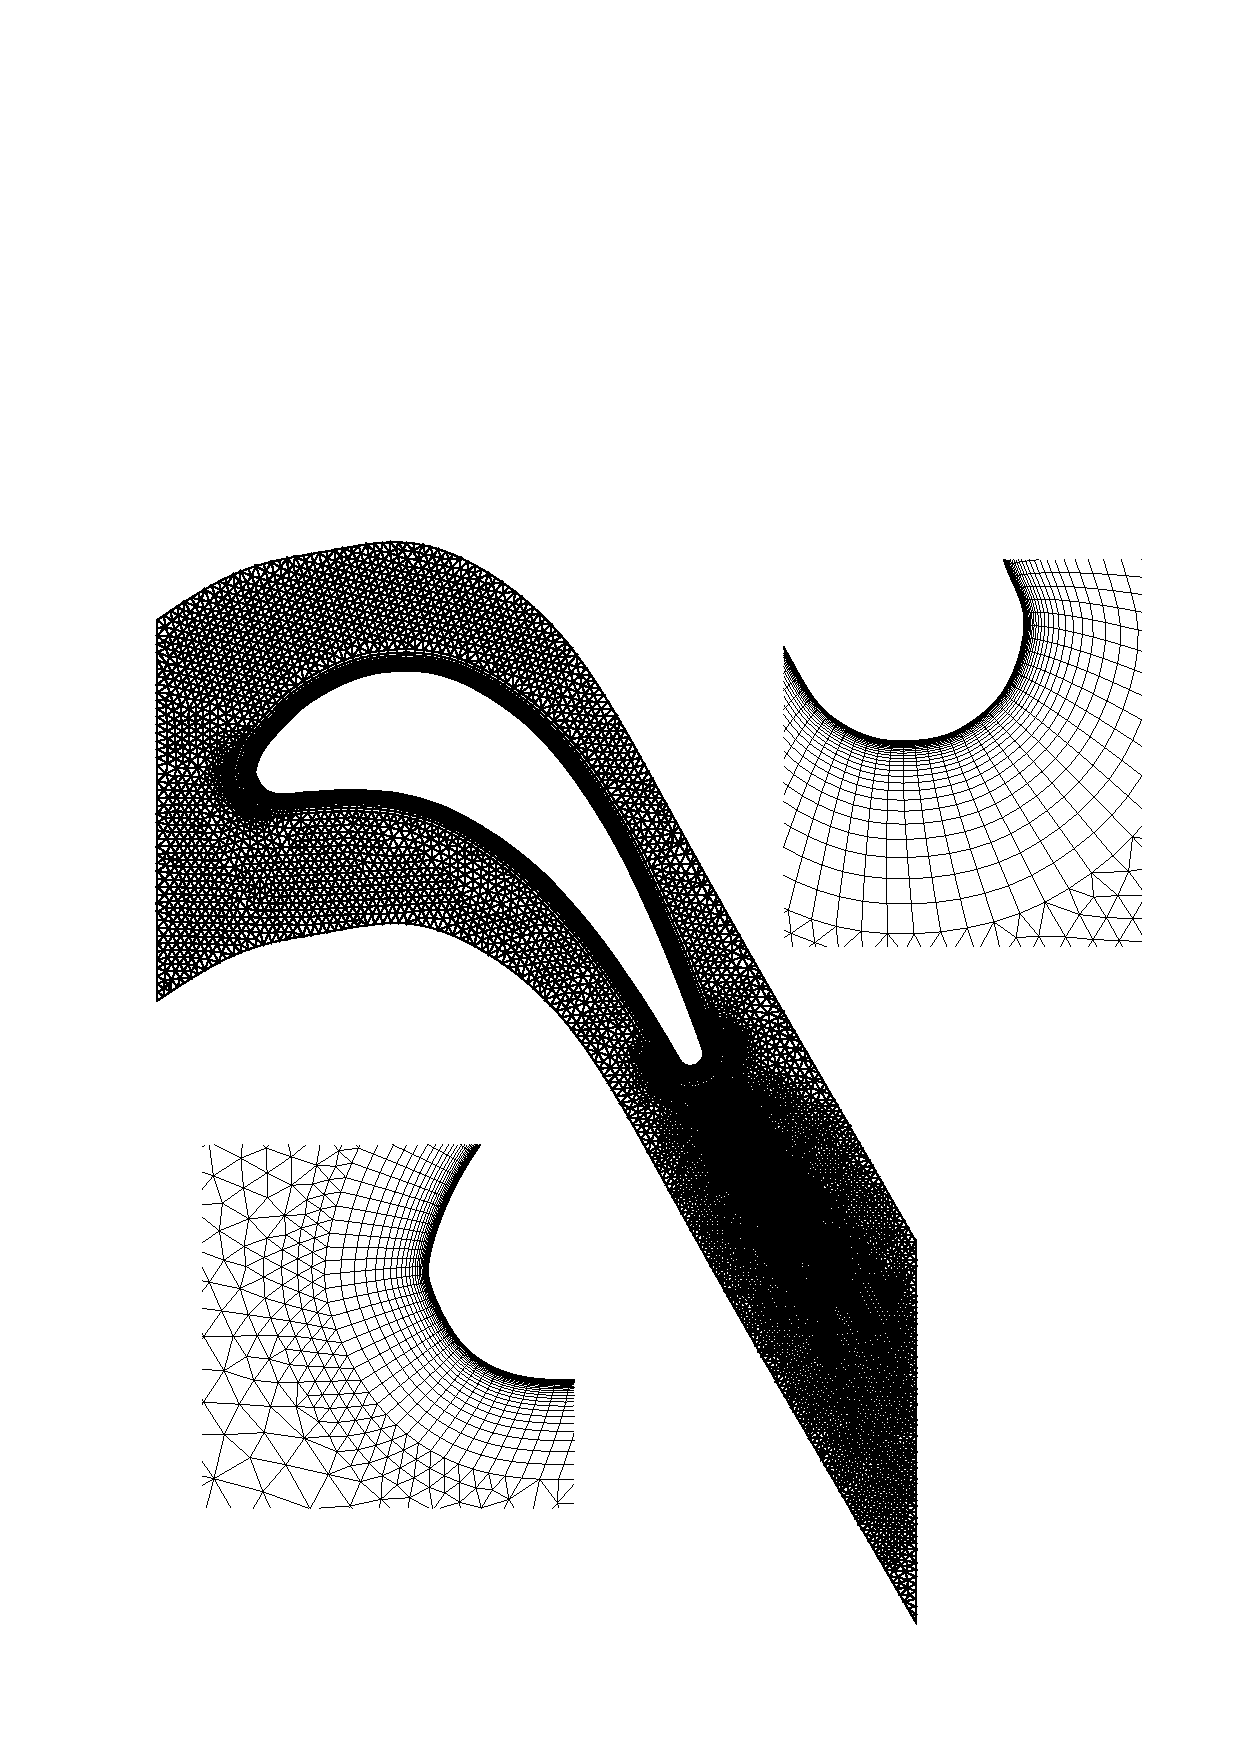
\includegraphics[width=110mm,clip=t]{CHAP_NONLIN/FIGURE/vki_mesh_1.pdf}}
 \caption{VKI LS59 rotor blade. Computational mesh with zoom views at leading- and
          trailing-edges}
 \label{vki_mesh_1.fig}
\end{figure}
%

 The inlet flow angle is $30\se{o}$ while the Reynolds number
 based on the blade chord and outlet conditions is in the range from
 $6.2\cdot10\se{5}$ up to $8.3\cdot10\se{5}$.
 A view of the computational mesh is shown in Fig. \ref{vki_mesh_1.fig}.
 This mesh contains 7,440 quadrilaterals in the boundary layer region and
 12,842 triangles in the rest of the domain which yields a total of 14,203 points.
%
%
\begin{figure}
 \begin{center}
  \begin{tabular}{ccc}
    \subfigure[Grid 2: 3587 cells]
       {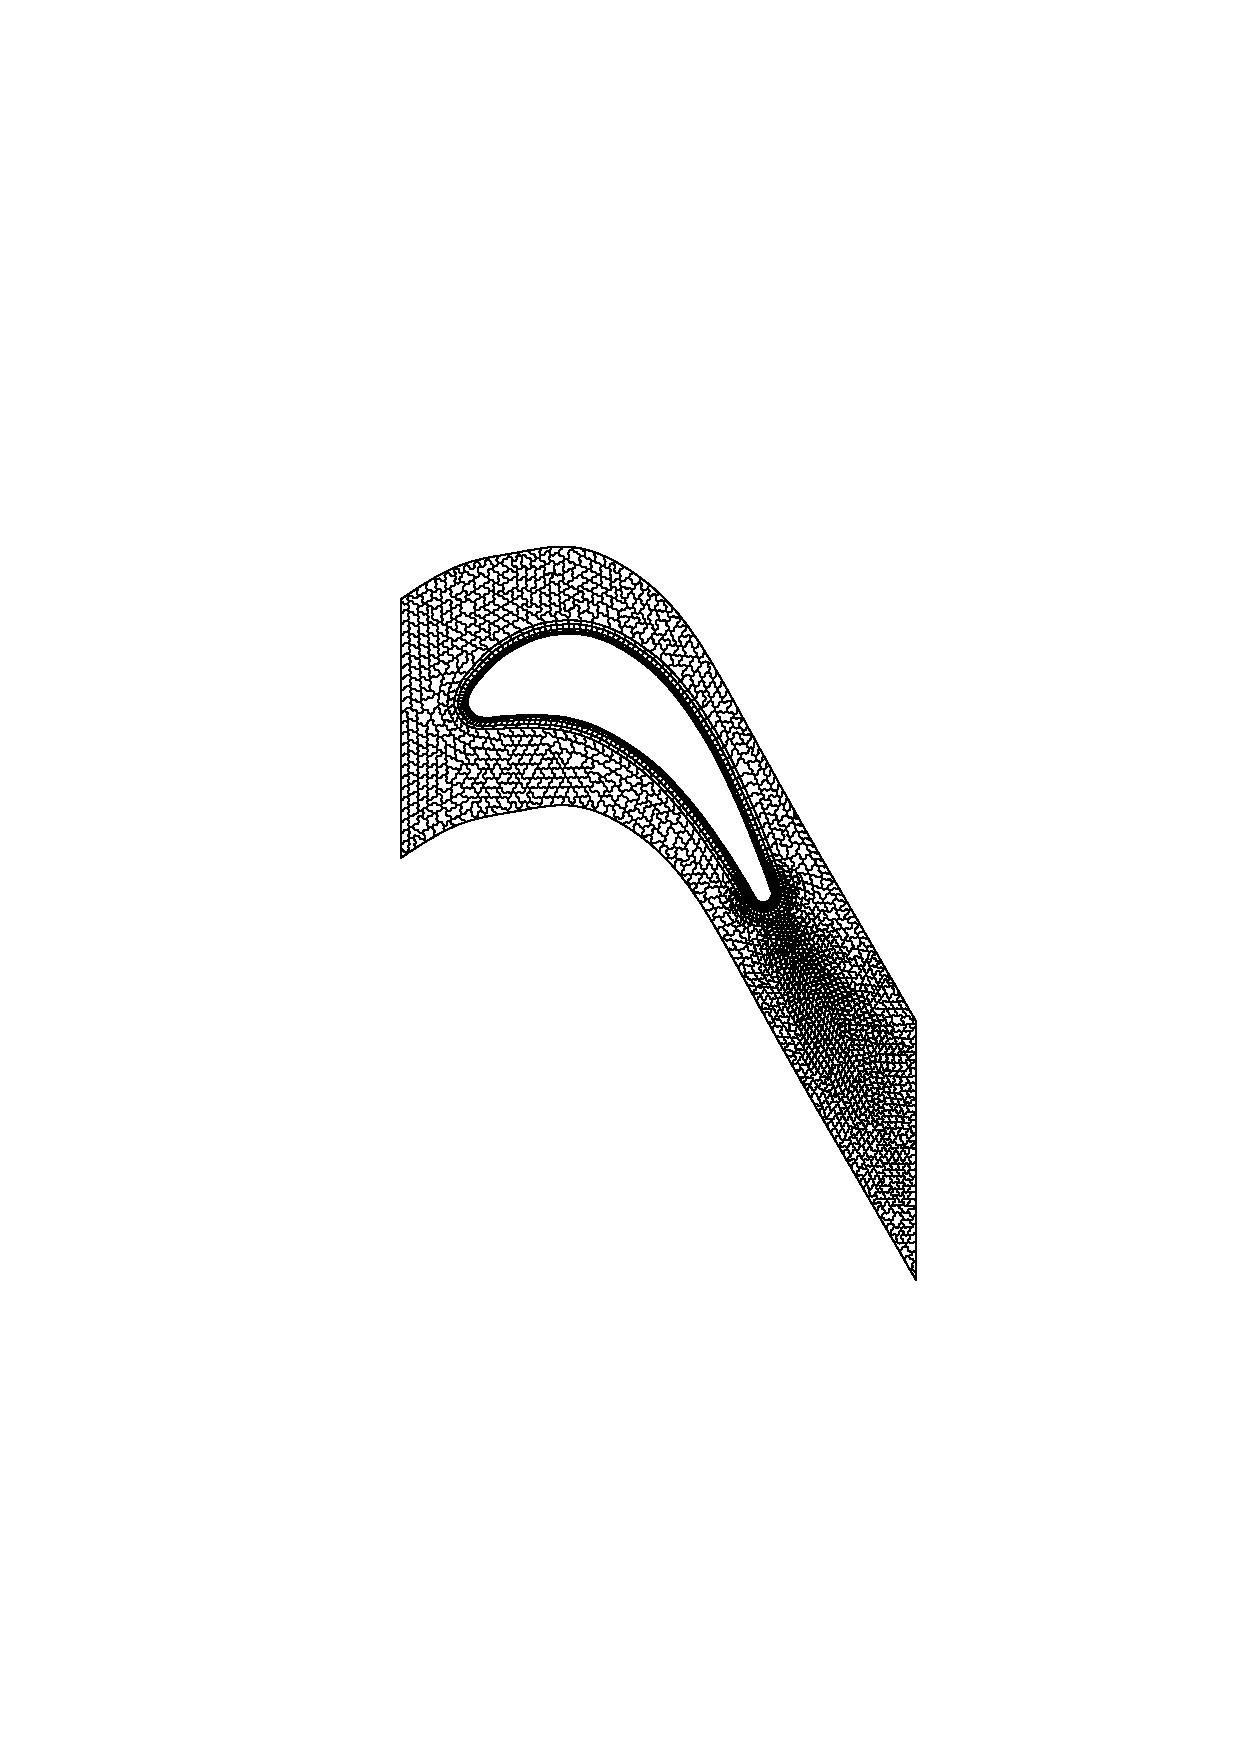
\includegraphics[width=45mm,clip=t]{CHAP_NONLIN/FIGURE/vki_mesh2.pdf}}
        &
    \subfigure[Grid 3: 908 cells]
       {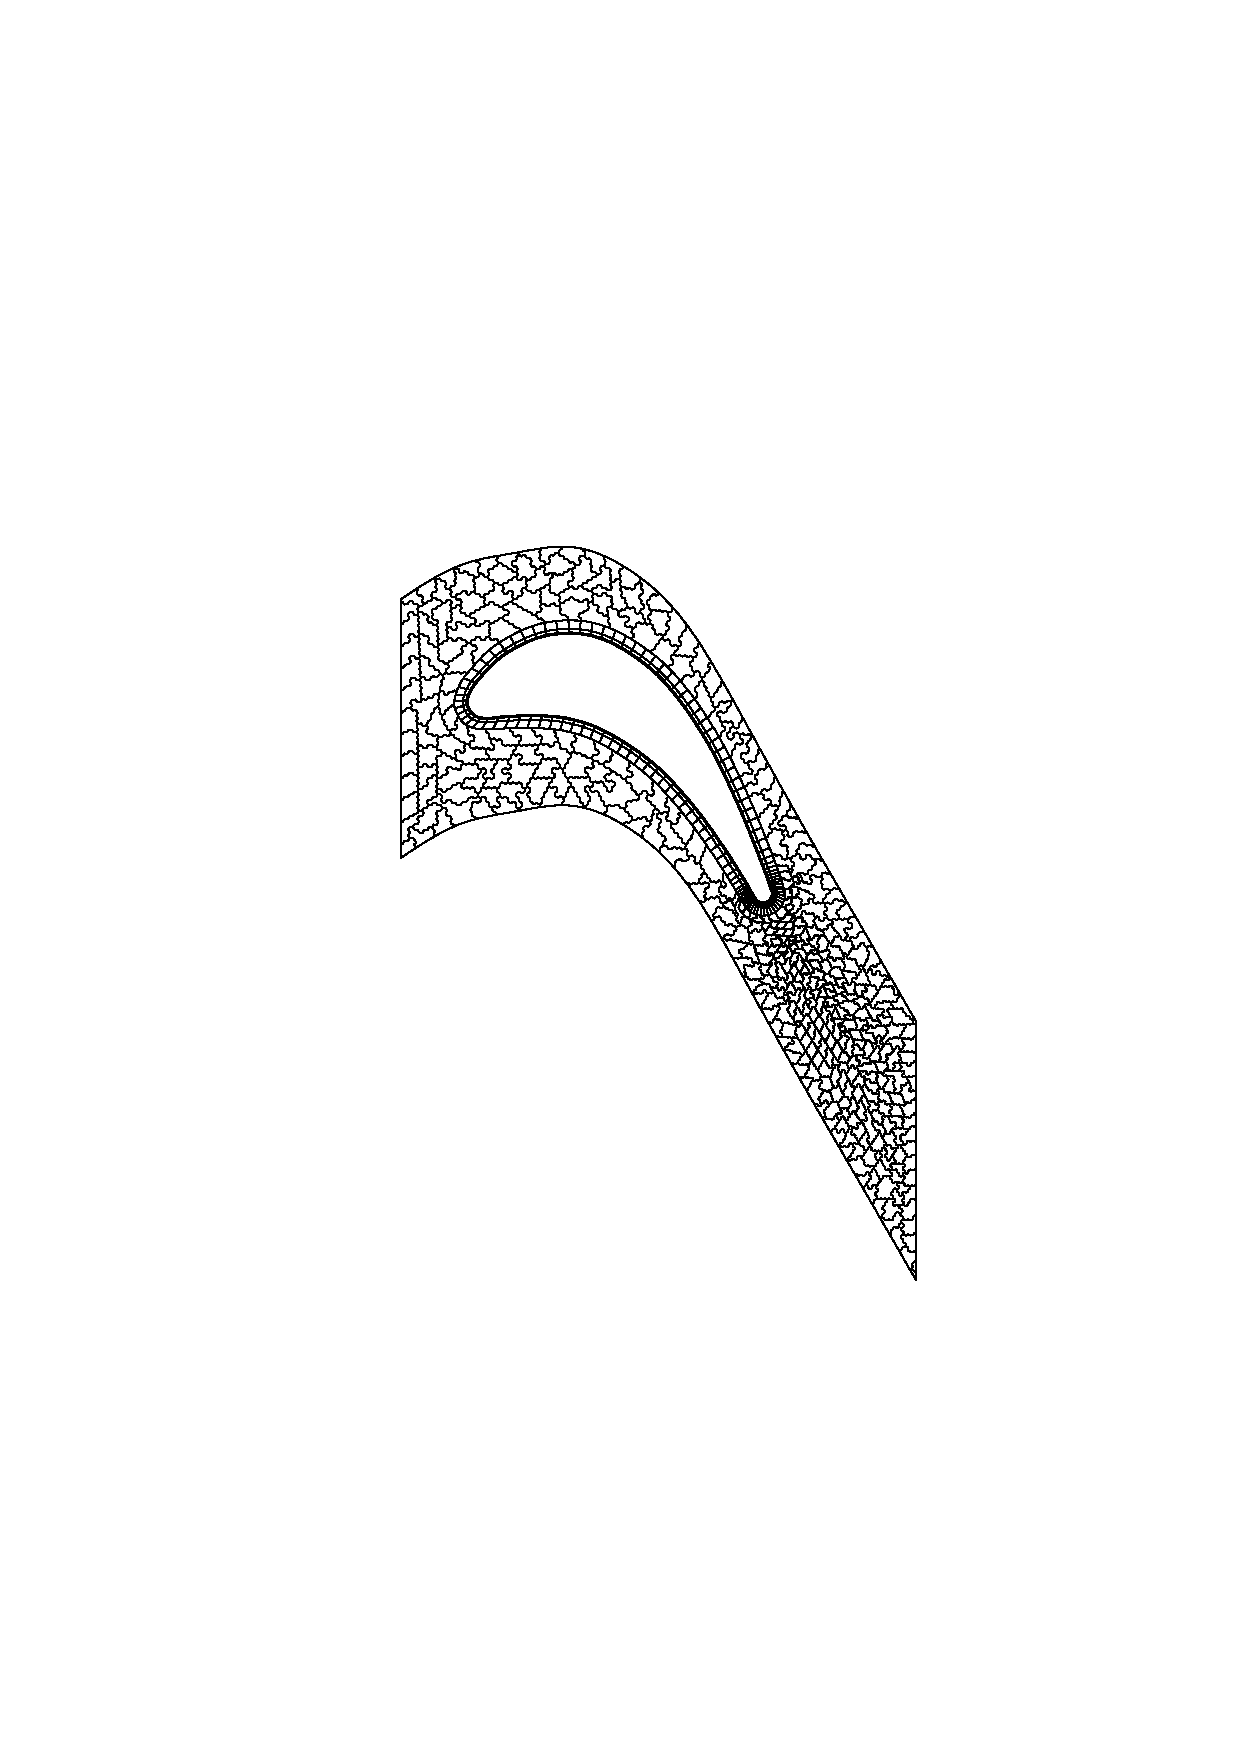
\includegraphics[width=45mm,clip=t]{CHAP_NONLIN/FIGURE/vki_mesh3.pdf}}
        &
    \subfigure[Grid 4: 239 cells]
       {\includegraphics[width=45mm,clip=t]{CHAP_NONLIN/FIGURE/vki_mesh4.pdf}}
  \end{tabular}
 \end{center}
 \vspace{-5mm}
 \caption{VKI LS59 rotor blade. Agglomerated grids}
 \label{vki_agglo.fig}
\end{figure}
%
 Three succesively agglomerated meshes were used in a four grid W-type cycle
 in conjunction with the line-implicit preconditioner described
 in Appendix \ref{multigrid.chap}.
 Fig. \ref{vki_agglo.fig} shows the control volumes associated with
 these agglomerated grids.
%
\begin{figure}
  \centerline{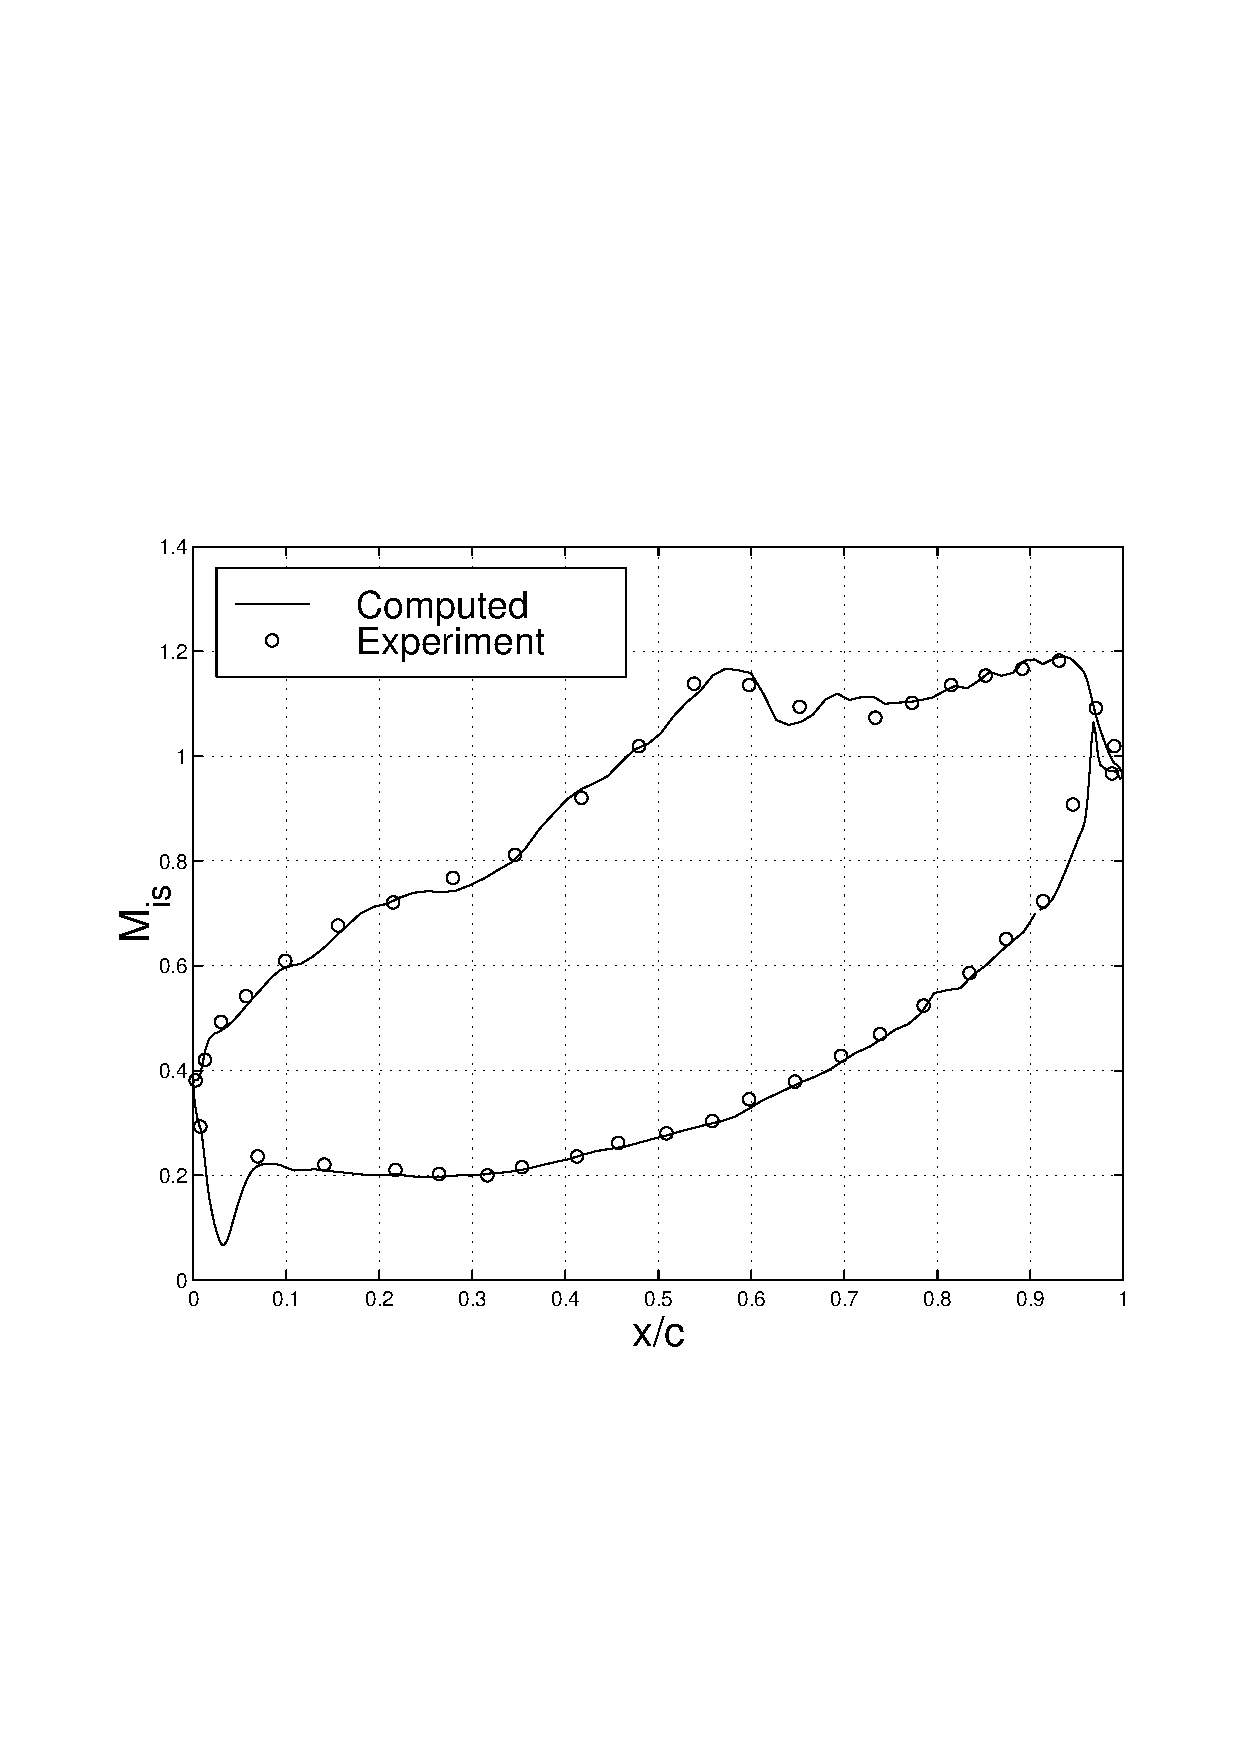
\includegraphics[width=130mm,clip=t]{CHAP_NONLIN/FIGURE/vki_blade.pdf}}
 \vspace{-5mm}
 \caption{VKI LS59 rotor blade. $M\sm{is2} = 1$, $Re\sm{2} = 7.6\cdot10\se{5}$.
          Isentropic Mach number distribution}
 \label{vki_mach_blade.fig}
\end{figure}
%
%
\begin{figure}
 \begin{center}
  \begin{tabular}{cc}
    \subfigure[Mach number contours]
       {\includegraphics[width=70mm,clip=t]{CHAP_NONLIN/FIGURE/vki_mach.pdf}}
        &
    \subfigure[Particle traces near the trailing edge]
       {\fbox{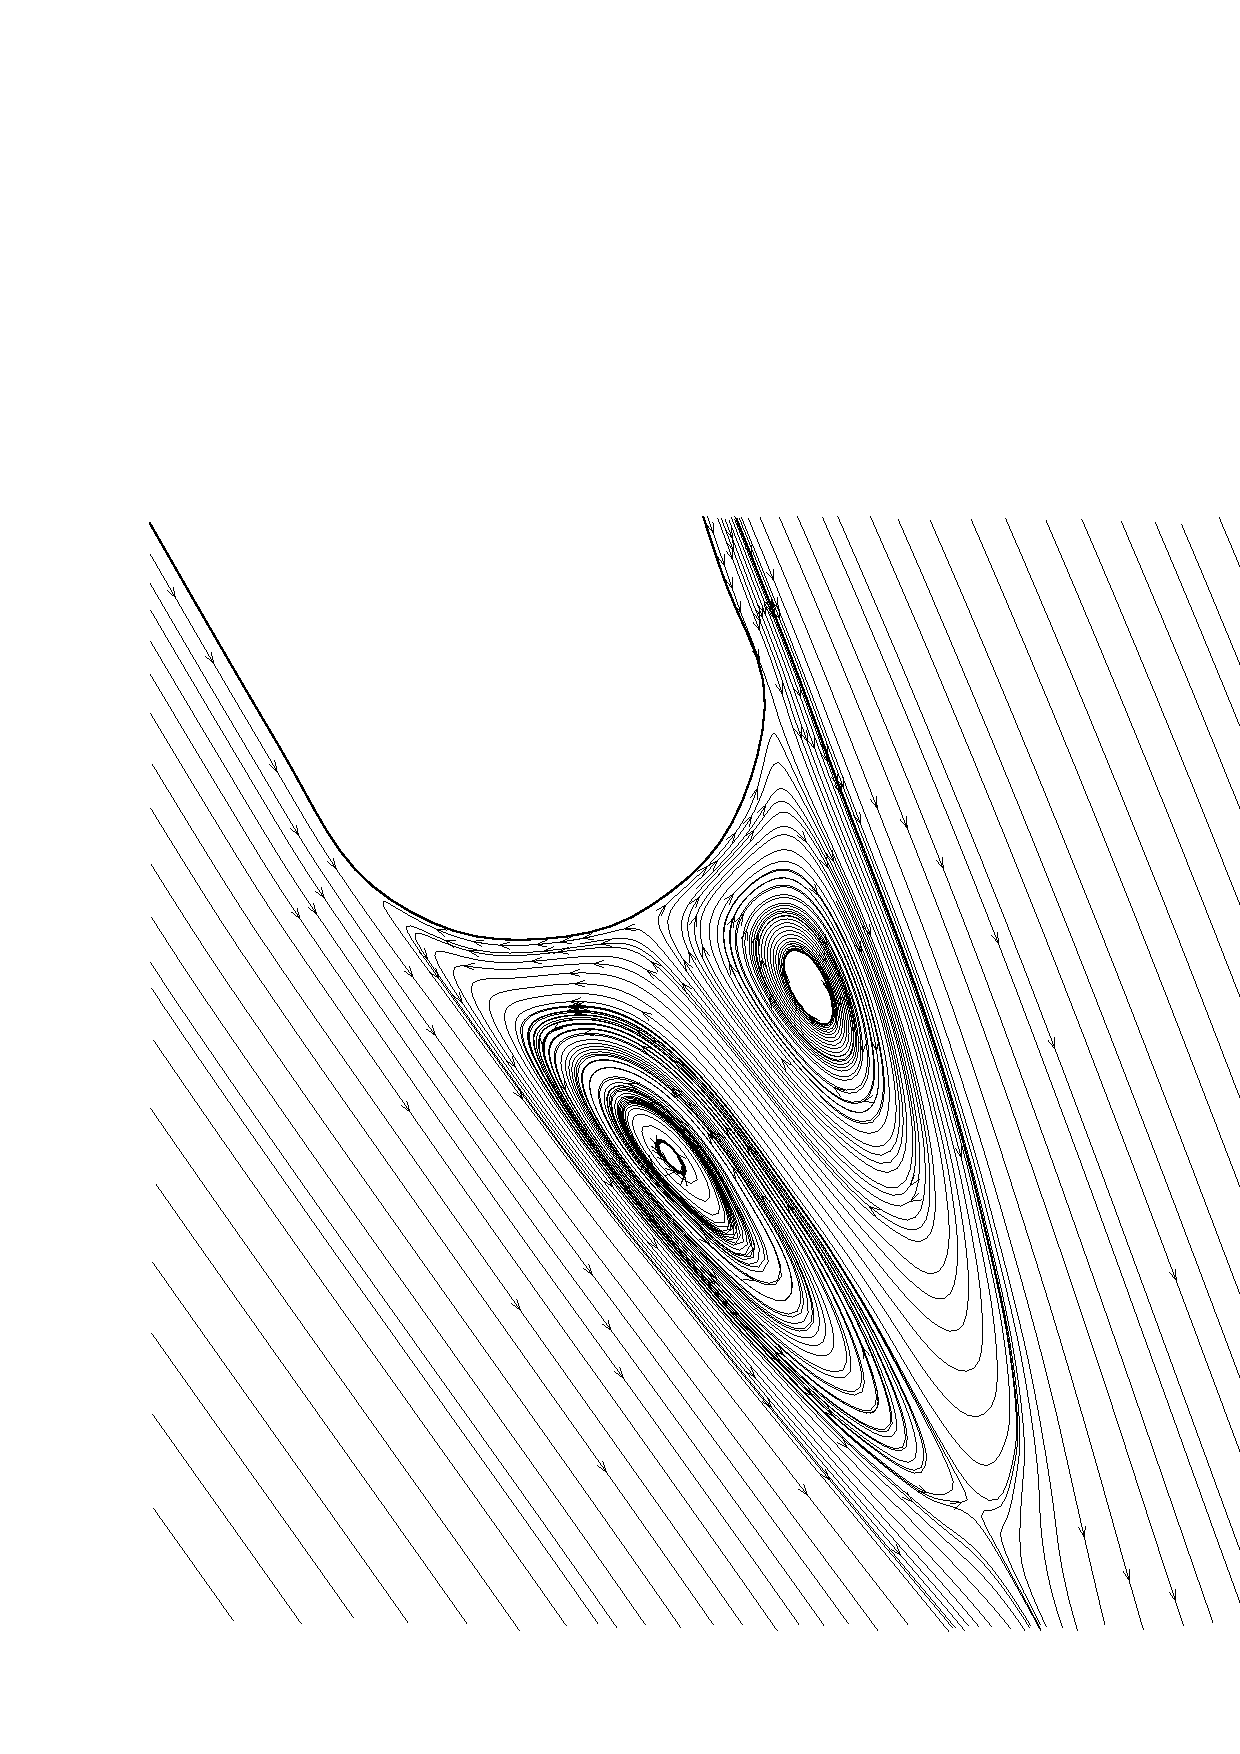
\includegraphics[width=70mm,clip=t]{CHAP_NONLIN/FIGURE/vki_traces.pdf}}}
  \end{tabular}
 \end{center}
 \vspace{-8mm}
 \caption{VKI LS59 rotor blade. $M\sm{is2} = 1$, $Re\sm{2} = 7.6\cdot10\se{5}$.
          Computed solution}
 \label{vki_mach.fig}
\end{figure}
%

 The isentropic Mach number distribution on the blade surface is given in
 Fig. \ref{vki_mach_blade.fig} for the case with an isentropic outlet Mach
 of unity. The sonic conditions are obtained at $x/c \approx 0.47$
 on the suction side and at the trailing edge in the pressure side
 resulting in fairly straight sonic line across the blade passage as
 shown in the Mach number contours of Fig. \ref{vki_mach.fig}a.
 The flow is accelerated along the suction side up to $x/c = 0.6$ followed
 by a moderate deceleration downstream.
 For this blade, the experimental data of
 Kiock et al. \citeyear{Kiock:1} include exit flow angles, inlet Mach number
 and loss coefficient defined as
 $\xi = 1 - \frac{\left|v\sm{2}\right|}{\left|v\sm{is2}\right|}$, where
 $v\sm{is2}$ represents the isentropic outlet velocity. The comparison
 between the experimental and the computed values of such quantities as a
 function of the outlet Mach number is reported in Fig. \ref{vki_blade.fig}.
%
%
\begin{figure}
 \begin{center}
  \begin{tabular}{c}
    \subfigure[Exit flow angle]
       {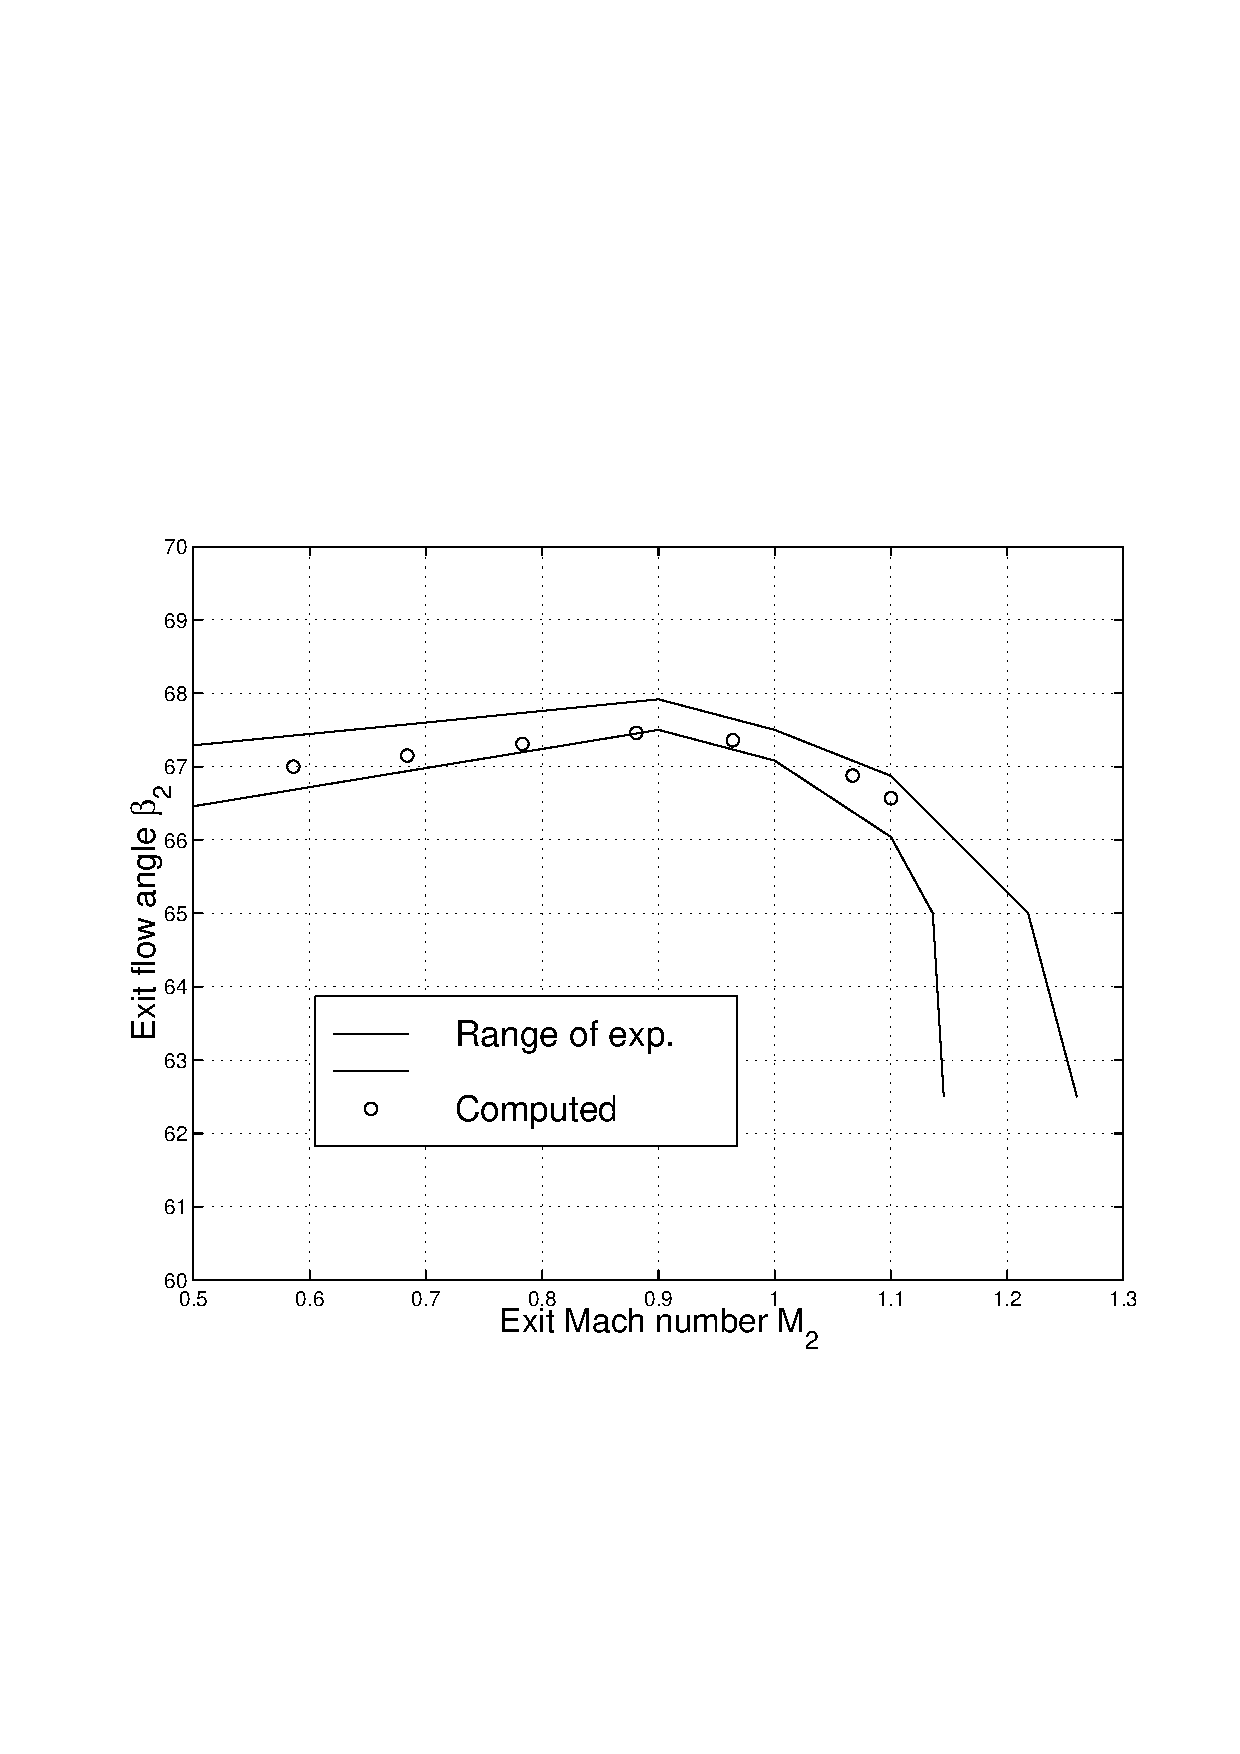
\includegraphics[width=80mm,clip=t]{CHAP_NONLIN/FIGURE/vki_beta2.pdf}}
        \vspace{-4mm}\\
    \subfigure[Inlet Mach number]
       {\includegraphics[width=80mm,clip=t]{CHAP_NONLIN/FIGURE/vki_mach1.pdf}}
        \vspace{-4mm}\\
    \subfigure[Loss coefficient]
       {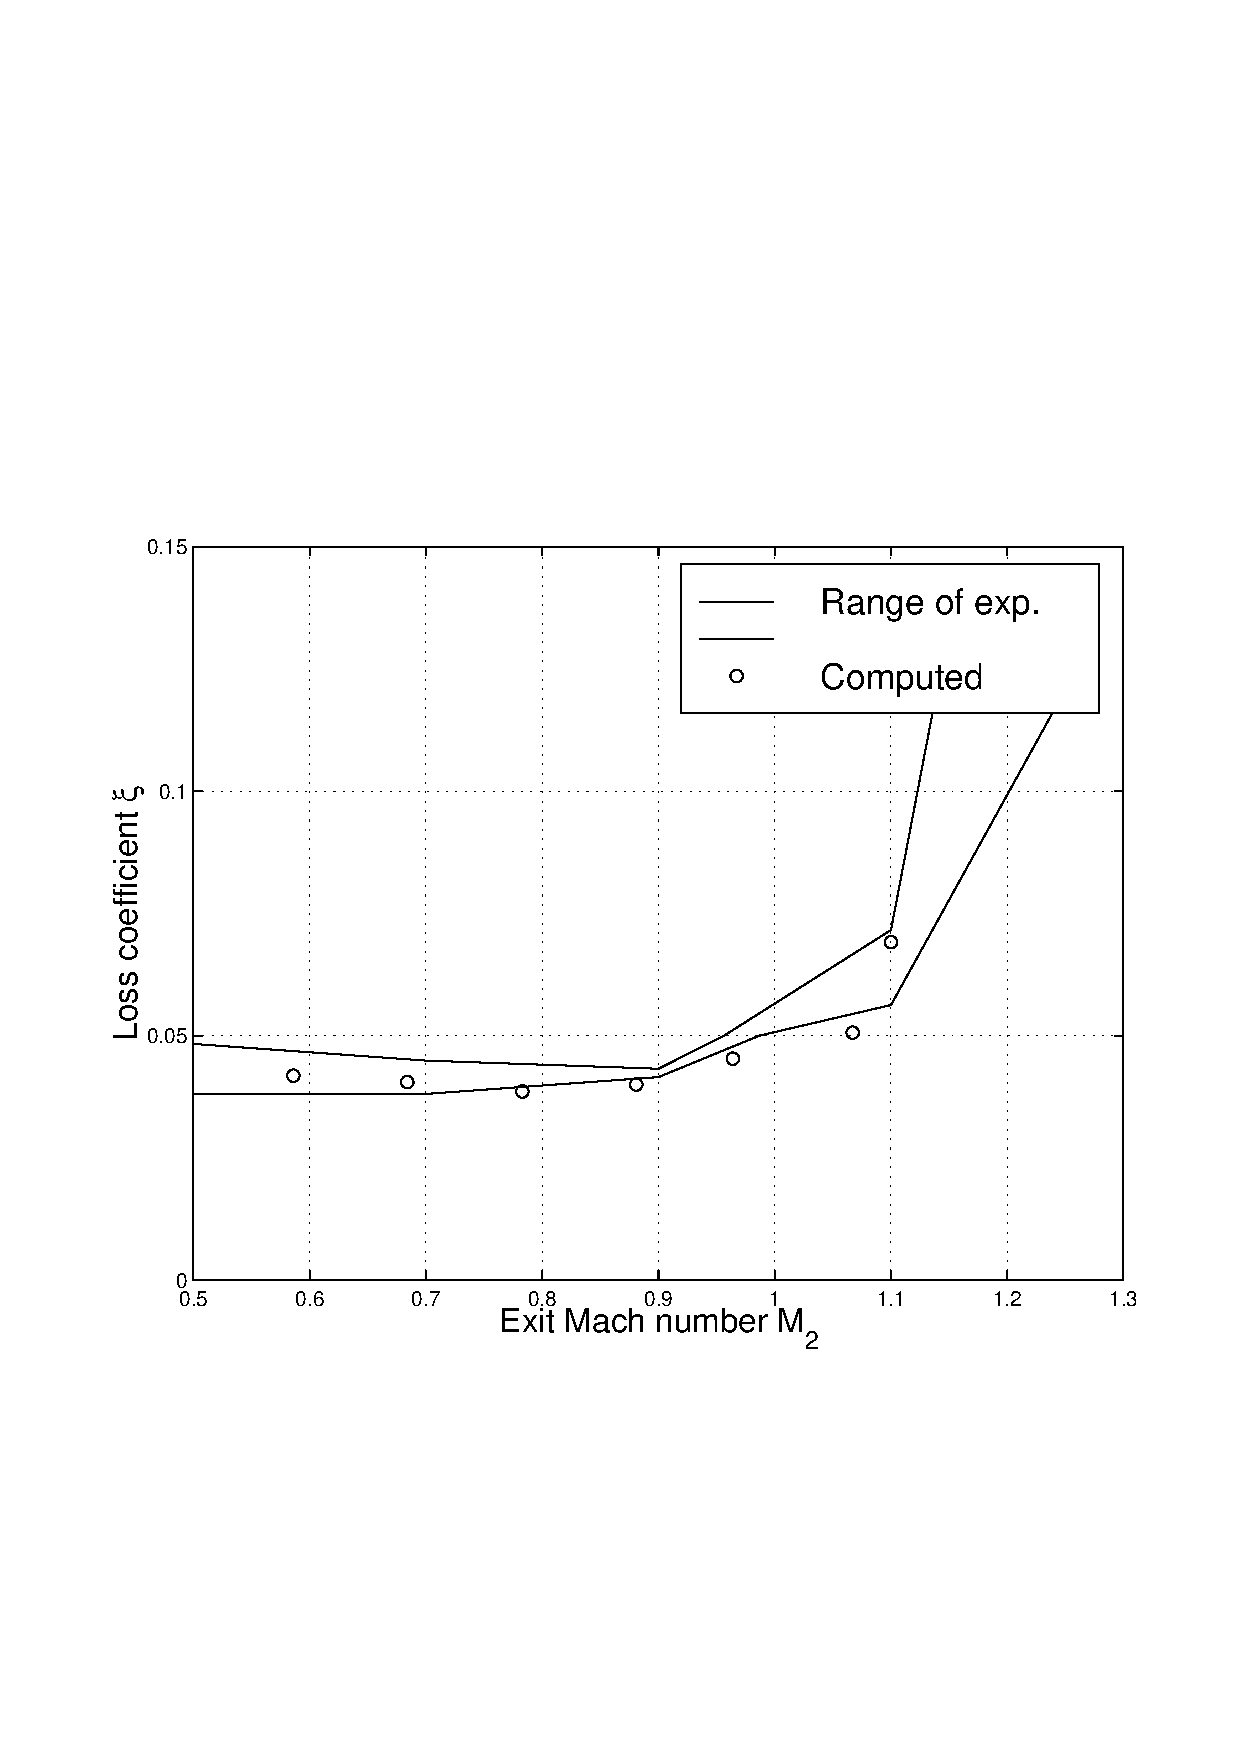
\includegraphics[width=80mm,clip=t]{CHAP_NONLIN/FIGURE/vki_loss.pdf}}
  \end{tabular}
 \end{center}
 \vspace{-8mm}
 \caption{VKI LS59 rotor blade. Computed solutions}
 \label{vki_blade.fig}
\end{figure}
%
%

 Fig. \ref{vki_res.fig} compares the convergence history obtained using the
 line-implicit solver of Appendix \ref{multigrid.chap}, on a single grid and
 on four grid W-type cycle. The convergence history
 of a single grid, point-Jacobi, iterative implicit scheme as the one
 used by Sayma et al. \citeyear{Luca:10}, is also plotted.
 It is evident that the single grid solution is not converged
 and the reason of this could be blamed to the grid anisotropy as well as
 to the blunt trailing edge of the blade which causes a recirculation bubble
 which could be inherently unsteady (Fig. \ref{vki_mach.fig}b).
 The single grid implicit scheme of Sayma et al. \citeyear{Luca:1} converges very slowly
 because not designed to be effective in damping error arising from highly stretched
 meshes.
%
\begin{figure}
 \centerline{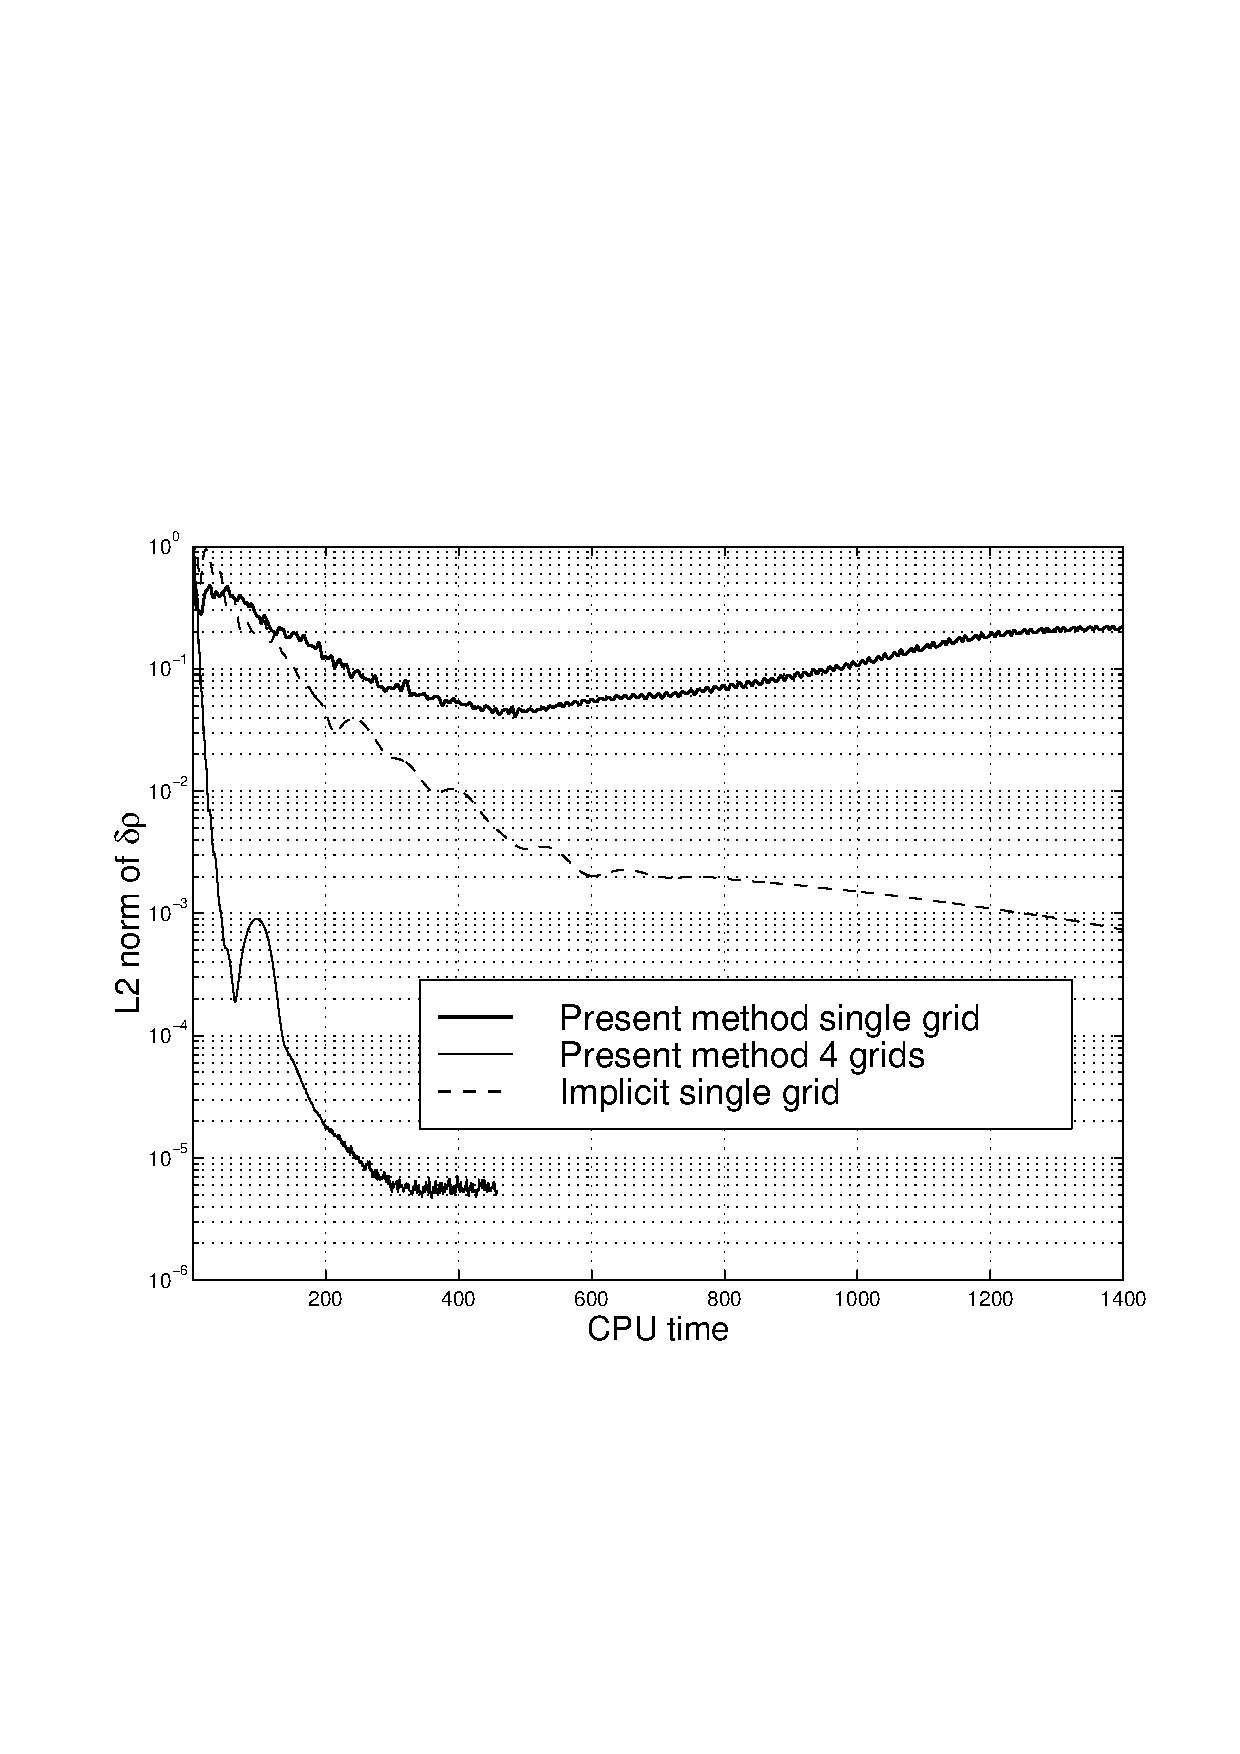
\includegraphics[width=130mm,clip=t]{CHAP_NONLIN/FIGURE/vki_res.pdf}}
 \caption{VKI LS59 rotor blade. Residual history}
 \label{vki_res.fig}
\end{figure}
%

%
%%
%
\subsection{NASA Rotor 37}
\label{nasa_rotor37.subsec}
%
 A low-aspect-ratio transonic inlet rotor for a core compressor,
 designated NASA rotor 37, was used in the present section to validate
 the steady state code for three-dimensional geometries.
 The rotor was originally designed and tested at NASA Lewis Research
 Center by Reid and Moore \citeyear{Reid:1}.
 In the CFD assessment, the rotor was tested in isolation by several
 researchers (Suder and Celestina \citeyearNP{Suder:1},
 Chima \citeyearNP{Chima:2}, Arima et al. \citeyearNP{Arima:1}).
 The rotor geometry together with the location measured using
 aerodynamics probes and laser anemometer measurements
 are shown in Fig. \ref{rot37_geo.fig}.
%
\begin{figure}
  \begin{center}
   \begin{tabular}{c}
    \subfigure
      {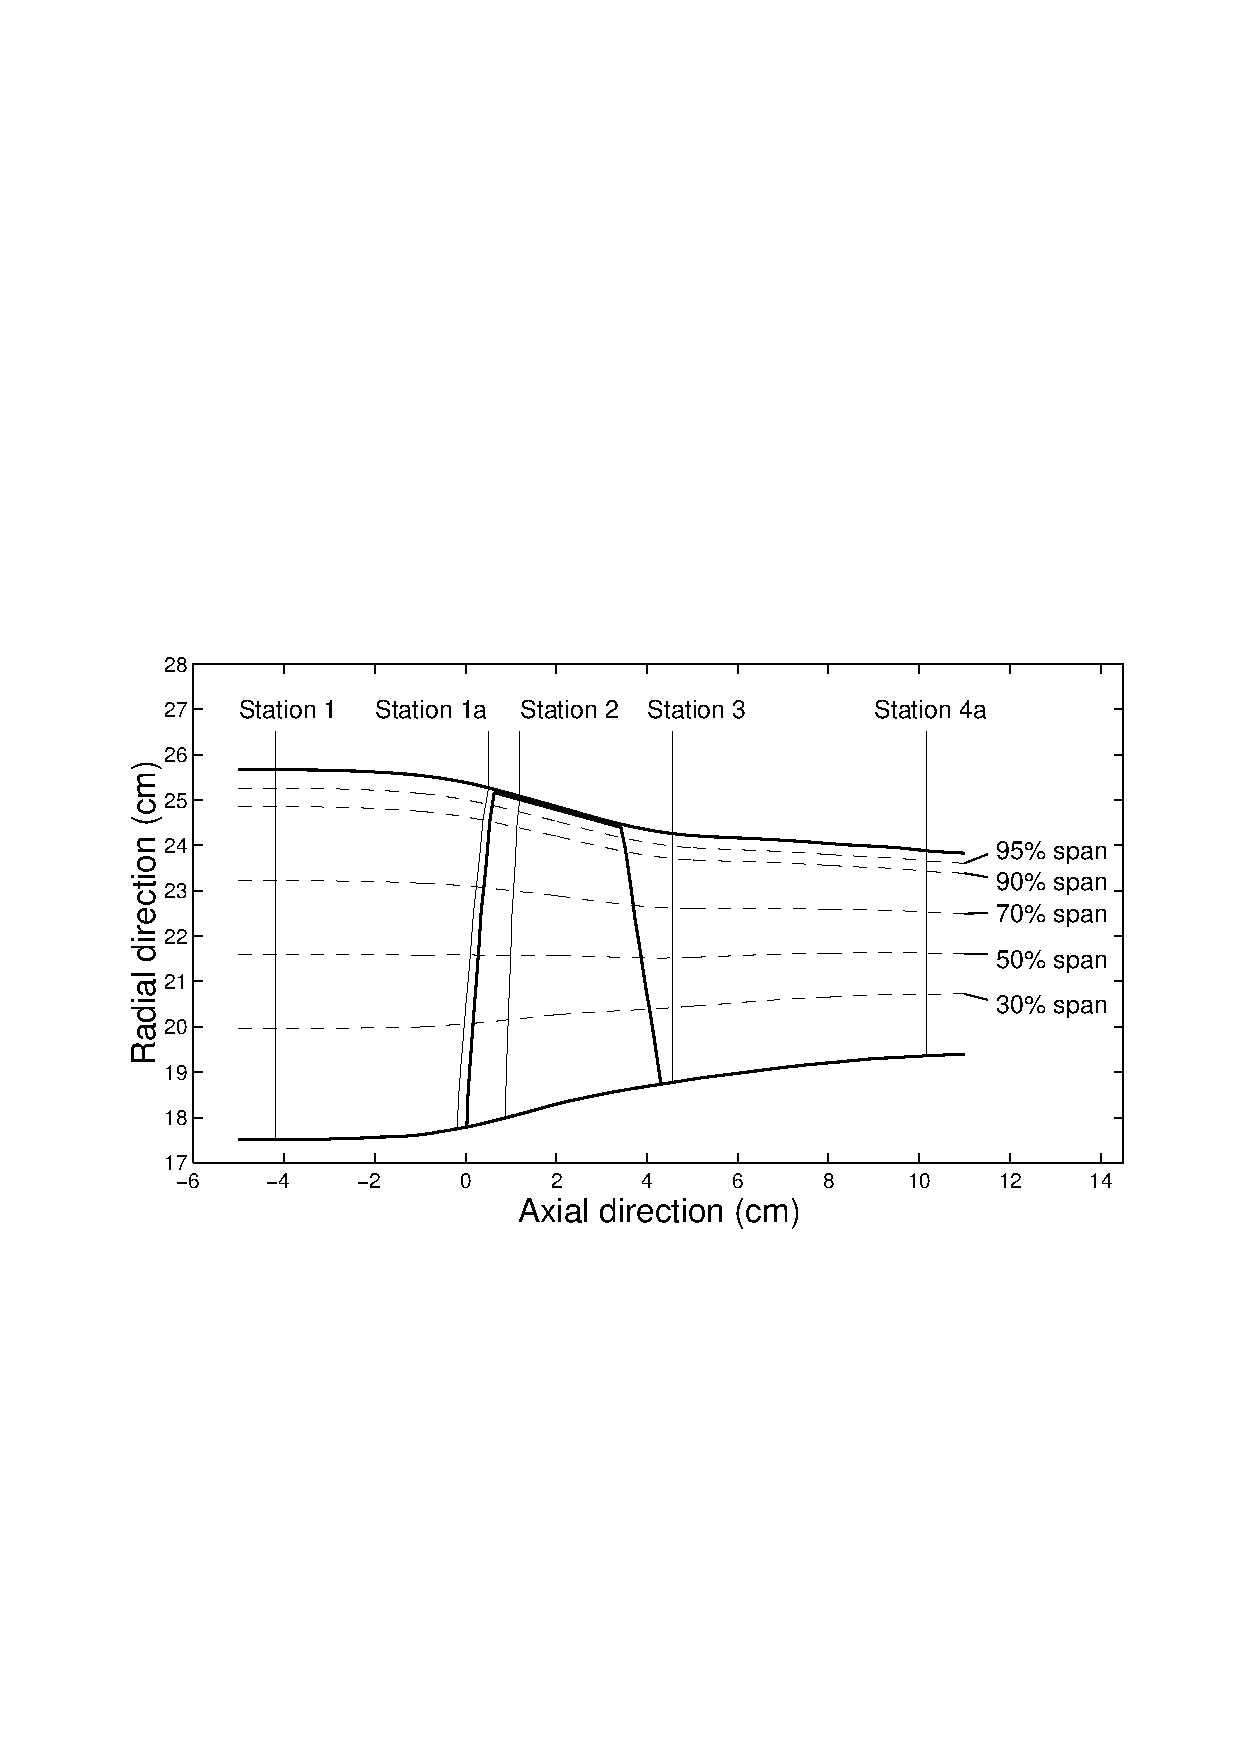
\includegraphics[width=100mm,clip=t]{CHAP_NONLIN/FIGURE/rotgeo.pdf}}
      \vspace{-4mm}\\
    \subfigure
      {\begin{tabular}{|c|c|c|c|c|c|}\hline
        Station & 1 & 1a & 2 & 3 & 4a \\ \hline
        x (cm) & -4.19 & $-5\%$ chord & $20\%$ chord & 4.57 & 10.16 \\ \hline
      \end{tabular}}
   \end{tabular}
  \end{center}
  \vspace{-8mm}
  \caption{NASA Rotor 37: $x-r$ view showing locations at which data were
           acquired}
  \label{rot37_geo.fig}
\end{figure}
%

 The rotor has a design pressure ratio of 2.106 at a mass flow of
 $20.19\ kg/s$, with a measured chocking mass flow of $20.93\ kg/s$.
 The rotor has 36 multiple-circular-arc blades with a hub-tip ratio
 of 0.7, an aspect ratio of 1.19, and a tip solidity
 of 1.288. The running tip clearance was estimated to be $0.356\ mm$
 ($0.45\%$ span). The design wheel speed is $17,188.7\ rpm$
 giving a nominal tip speed of $454\ m/s$.
 A brief description of the test facility and laser anemometer
 system is given by Suder and Celestina \citeyear{Suder:1}.

%
\begin{figure}
 \begin{center}
  \begin{tabular}{cc}
    \subfigure[Frontal view]
       {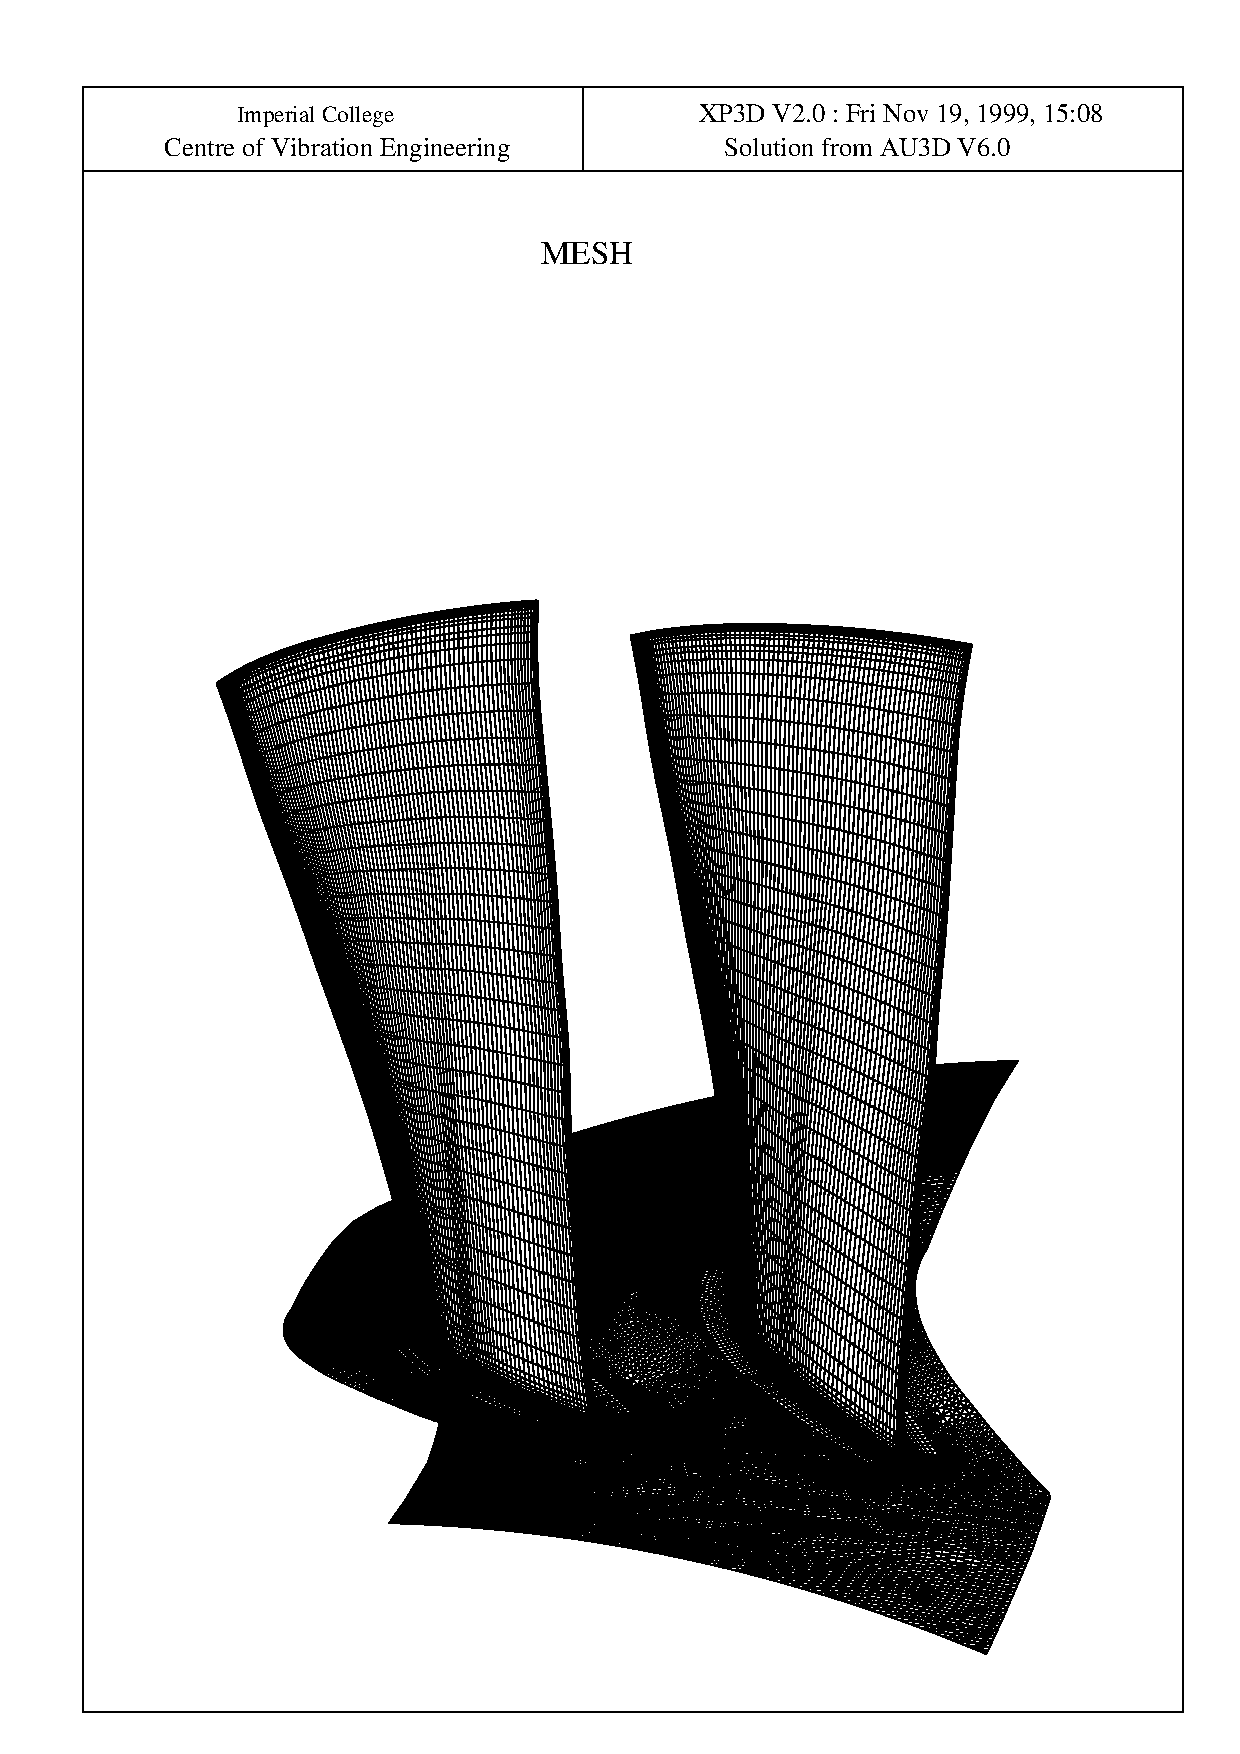
\includegraphics[width=55mm,clip=t]{CHAP_NONLIN/FIGURE/rot37_mesh1.pdf}}
        &
    \subfigure[$x-r\theta$ view]
       {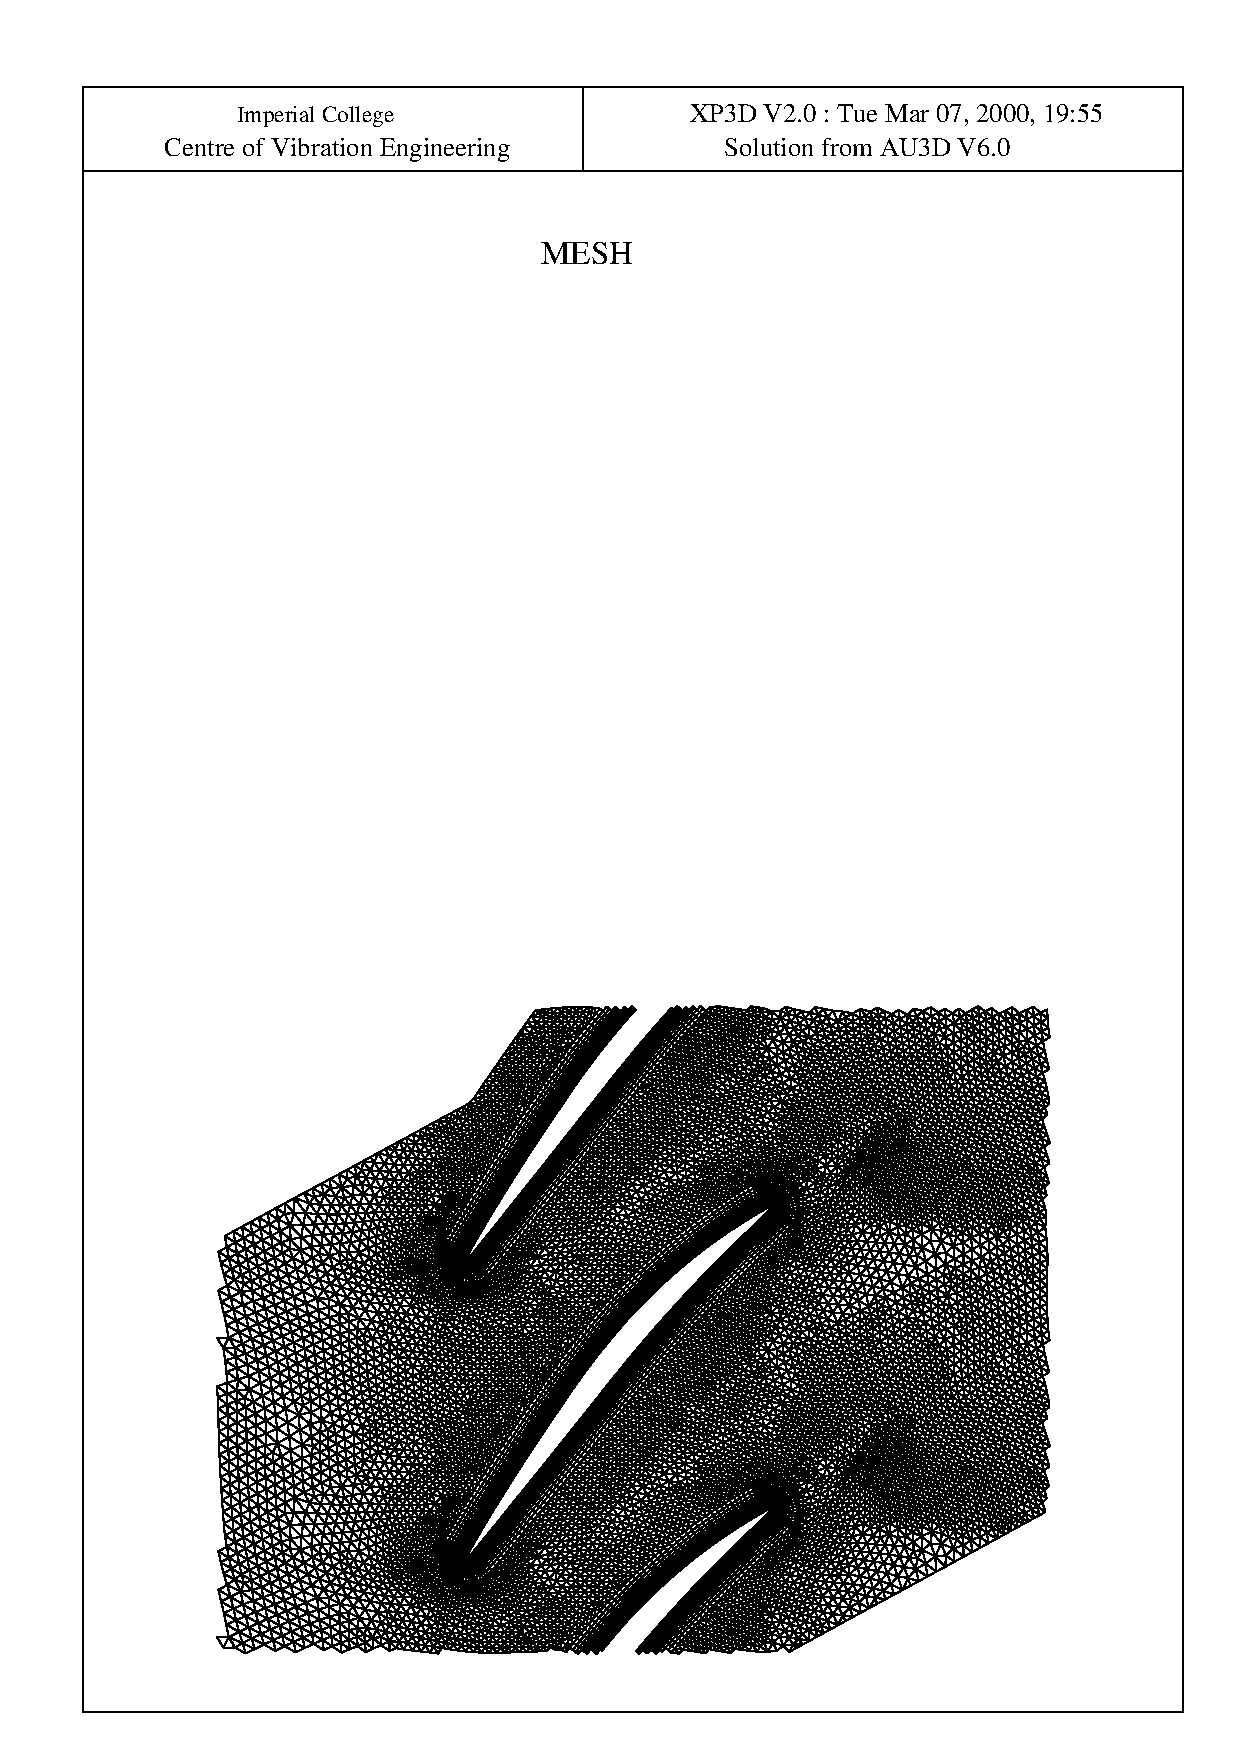
\includegraphics[width=85mm,clip=t]{CHAP_NONLIN/FIGURE/rot37_mesh4.pdf}}
      \vspace{-4mm}\\
    \subfigure[Tip gap view]
       {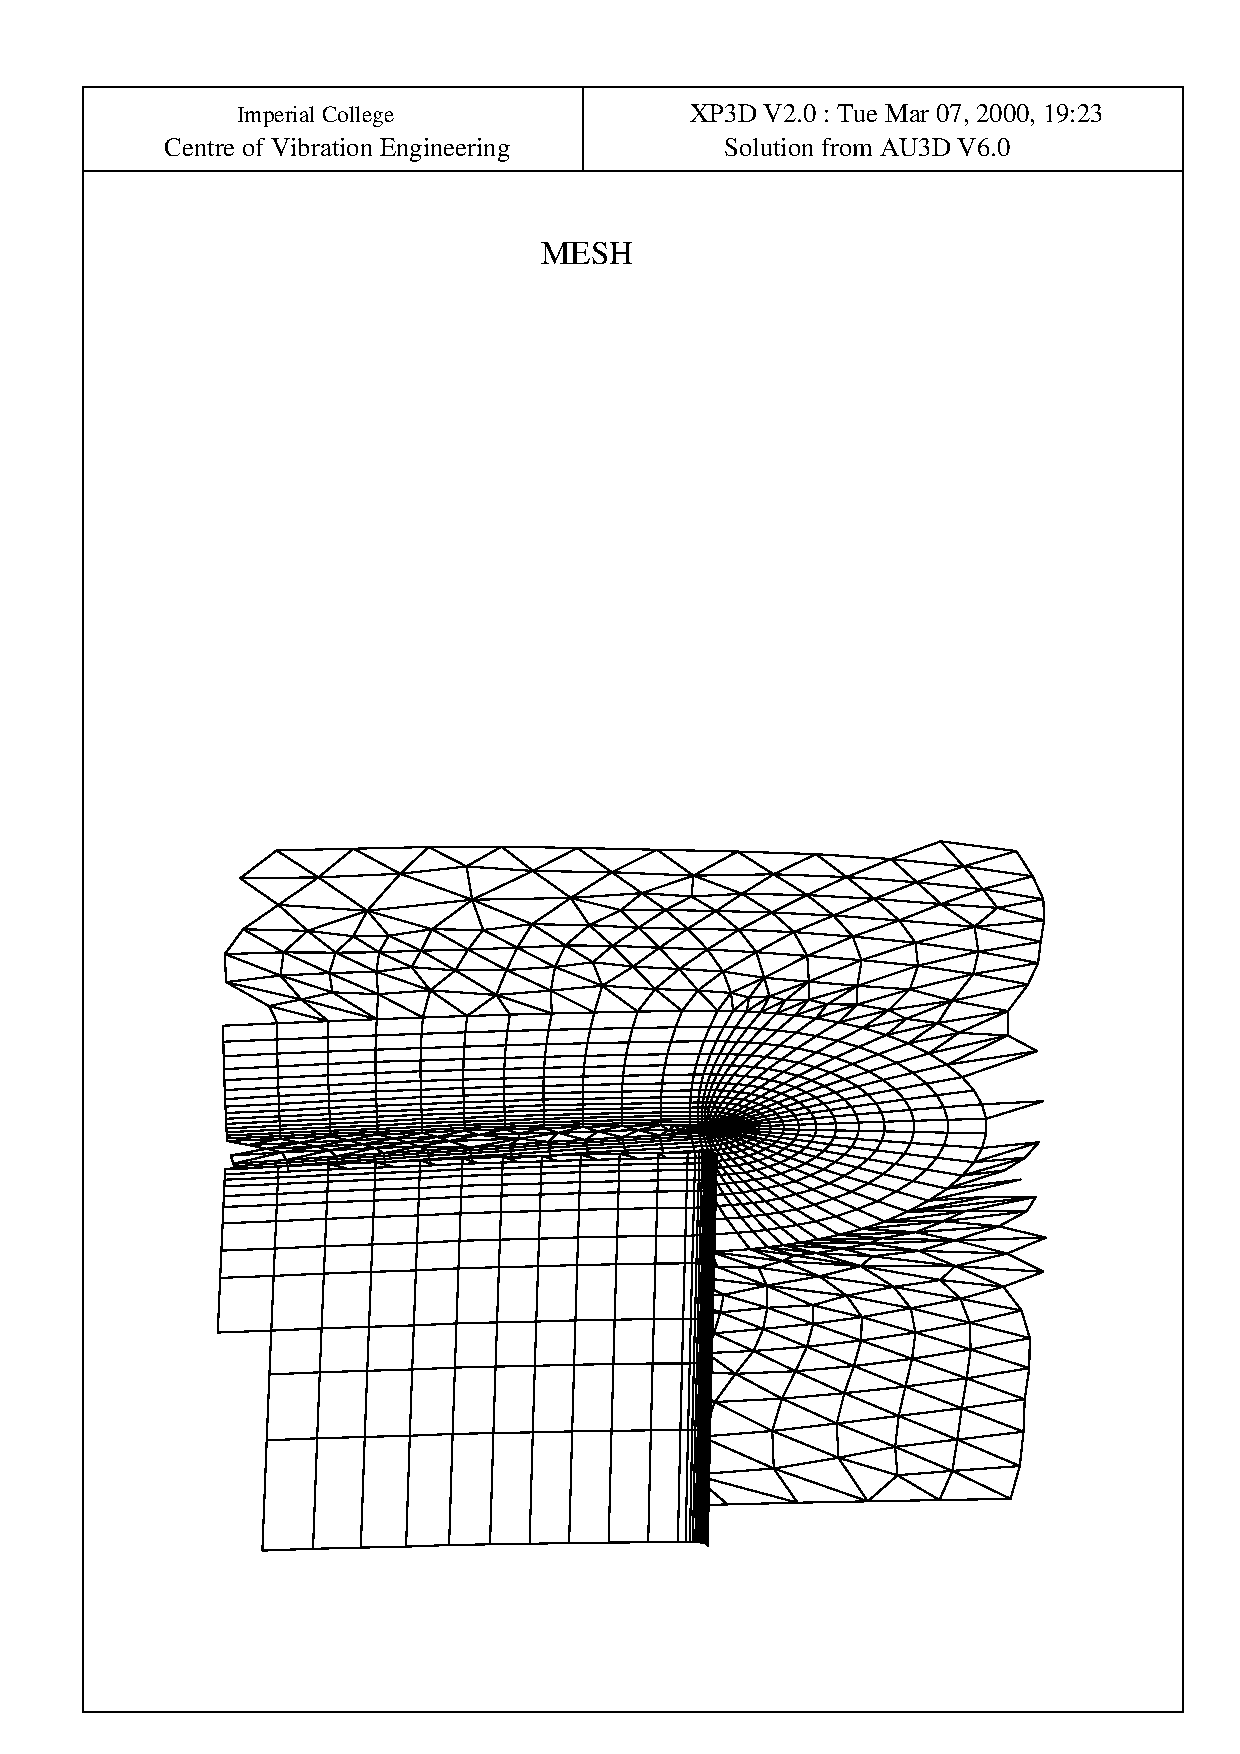
\includegraphics[width=55mm,clip=t]{CHAP_NONLIN/FIGURE/rot37_mesh3.pdf}}
        &
    \subfigure[$x-r$ view]
       {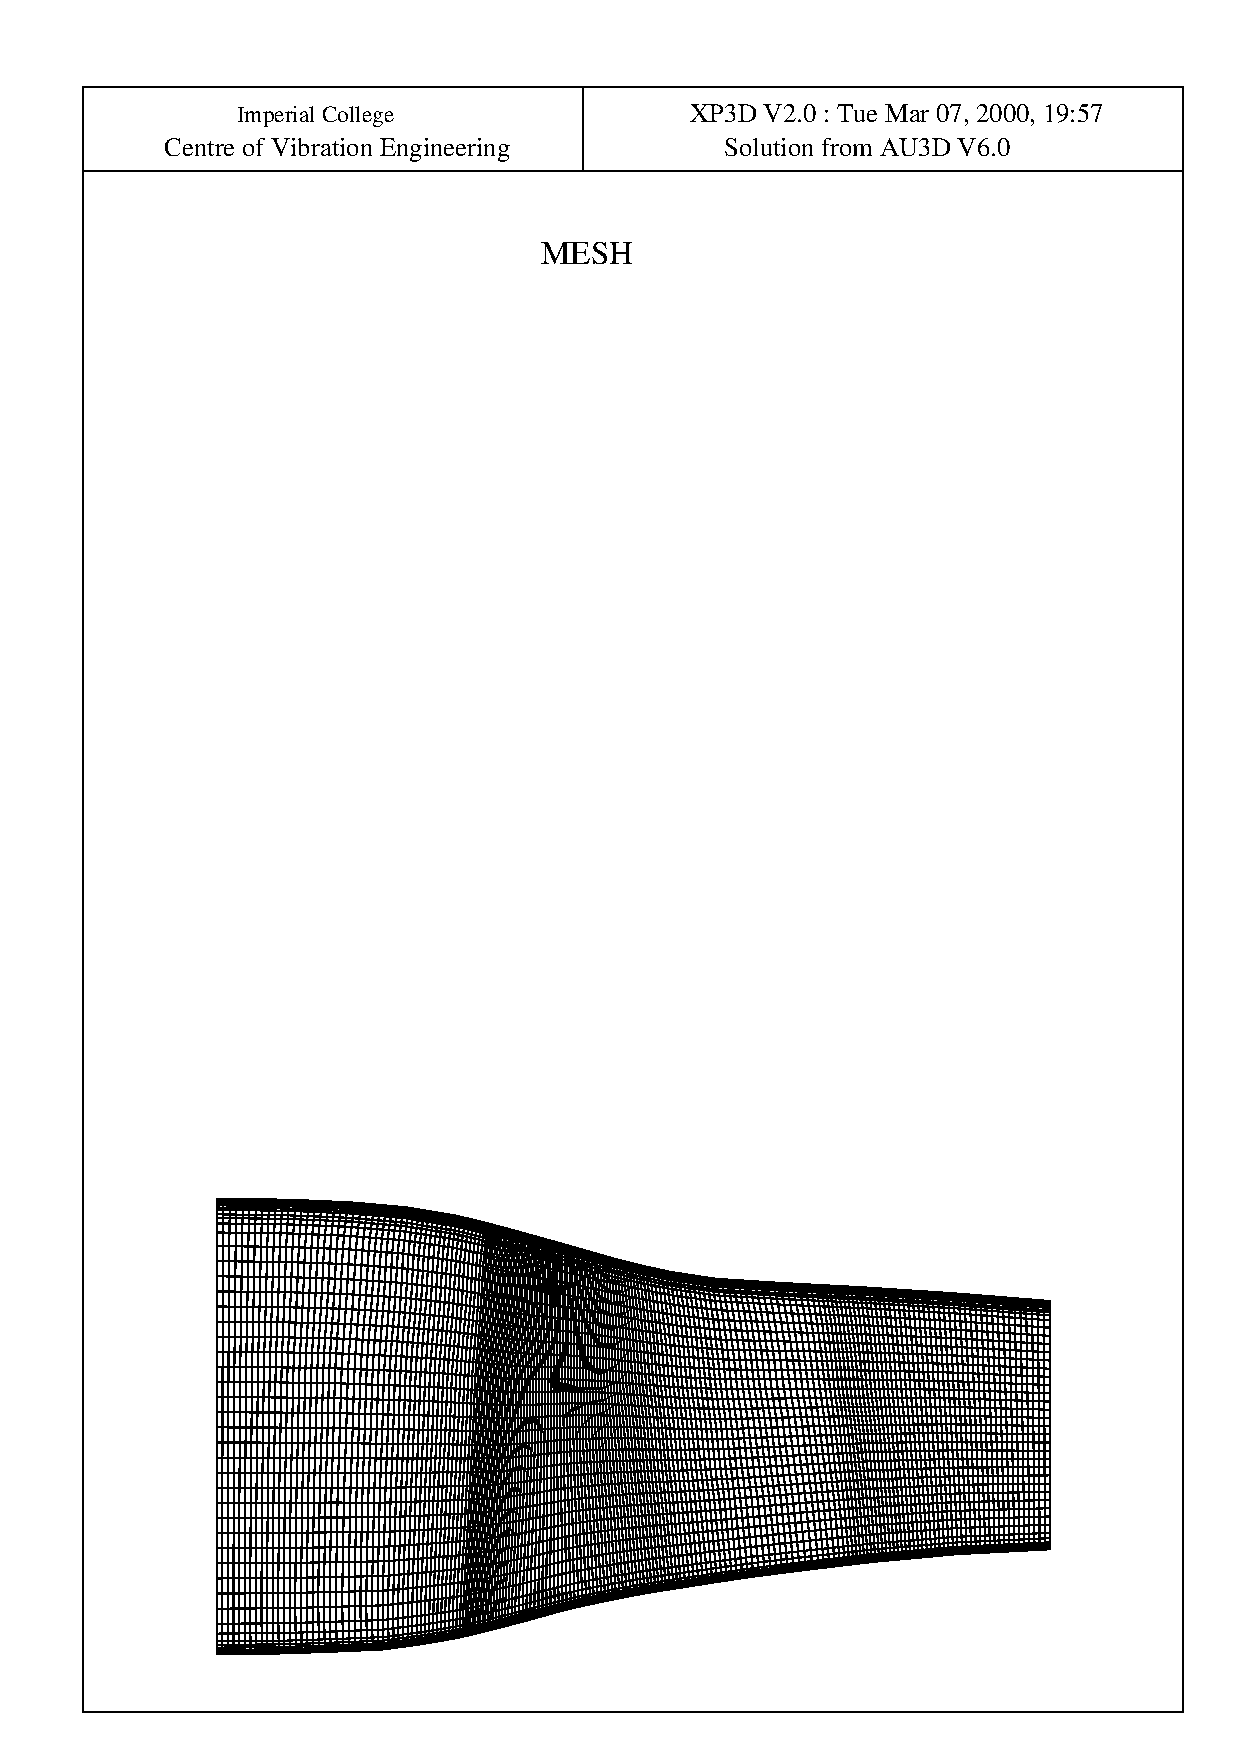
\includegraphics[width=85mm,clip=t]{CHAP_NONLIN/FIGURE/rot37_mesh2.pdf}}
  \end{tabular}
 \end{center}
 \vspace{-8mm}
 \caption{NASA Rotor 37: computational mesh}
 \label{rot37_mesh.fig}
\end{figure}
%
 Views of the computational mesh,
 generated with the semi-structured mesh generator
 LEVMAP described in chapter \ref{mesh.chap}
 (Sbardella et al. \citeyearNP{Luca:9}),
 are shown in Fig. \ref{rot37_mesh.fig}.
 The computational domain extends axially from station 1 in Fig.
 \ref{rot37_geo.fig} up to $x=10.67\ cm$ which corresponds to
 station 4 (not shown in Fig. \ref{rot37_geo.fig}). It contains 174,900 hexahedra
 in the boundary layer reagion and 607,067 wedges in the rest of the domain for
 a total number of point of 504,946. The boundary layer mesh does not resolve
 the viscous sublayer thus calculations with wall-slip condition
 (\ref{flow_tangency1.eq}) and wall-shear
 stresses evaluated using the low of the wall are considered here.
 As shown in Fig. \ref{rot37_geo.fig}c, the tip clearance flows will be modelled
 in a straightforward way by simply meshing the gap and setting the rotation
 speed at the casing to zero.
 At the hub section the reagion $x < -0.264\ cm$, $x > 4.521\ cm$,
 is not rotating so the rotational speed is also set to zero.
%
\begin{figure}
 \begin{center}
  \begin{tabular}{cc}
    \subfigure[$95\%$ span]
       {\includegraphics[width=60mm,clip=t]{FIGURE/CHAP2/rot37_cont_95.pdf}}
        &
    \subfigure[$97\%$ span]
       {\includegraphics[width=60mm,clip=t]{FIGURE/CHAP2/rot37_cont_97.pdf}}
       \vspace{-4mm} \\
    \subfigure[$99\%$ span]
       {\includegraphics[width=60mm,clip=t]{FIGURE/CHAP2/rot37_cont_99.pdf}}
        &
    \subfigure[Tip gap]
       {\includegraphics[width=60mm,clip=t]{FIGURE/CHAP2/rot37_cont_gap.pdf}}
  \end{tabular}
 \end{center}
 \vspace{-8mm}
 \caption{Rotor 37: Mach number contours}
 \label{rot37_mach.fig}
\end{figure}
%

%
%
%
%
\subsection{Impulsively accelerated flat plate}
\label{accelerated_flat_plate.subsec}
%
 To demonstrate the capability of the present method for unsteady flow,
 the solution of an impulsively accelerated flat plate in the laminar regime
 is presented. This example is also known as Stokes first problem
 and an analytical solution for incompressible flow is available
 (Schlichting \citeyearNP{Schlichting}, Mattioli \citeyearNP{Mattioli:1}).
 This analytical solution shows that the time dependent
 solution collapses to a single solution of nondimensional velocity versus
 the similarity parameter $\eta$ defined as

%
\beq
  \eta = \frac{y}{2\sqrt{\nu t}}
  \label{stokes_first1.eq}
\eeq
%
 where $y$ is the normal distance from the flat plate, $\nu$ is the kinematic
 viscosity and $t$ is the physical time. The analytical solution take the
 simple form

%
\beq
  \frac{u}{u_\infty} = {\tt erf}\left(\eta\right)
  \label{stokes_first2.eq}
\eeq
%
 where $\tt erf$ represents the error function (Schlichting \citeyearNP{Schlichting}).
%
\begin{figure}
 \begin{center}
  \begin{tabular}{c}
    \subfigure[Velocity profiles]
       {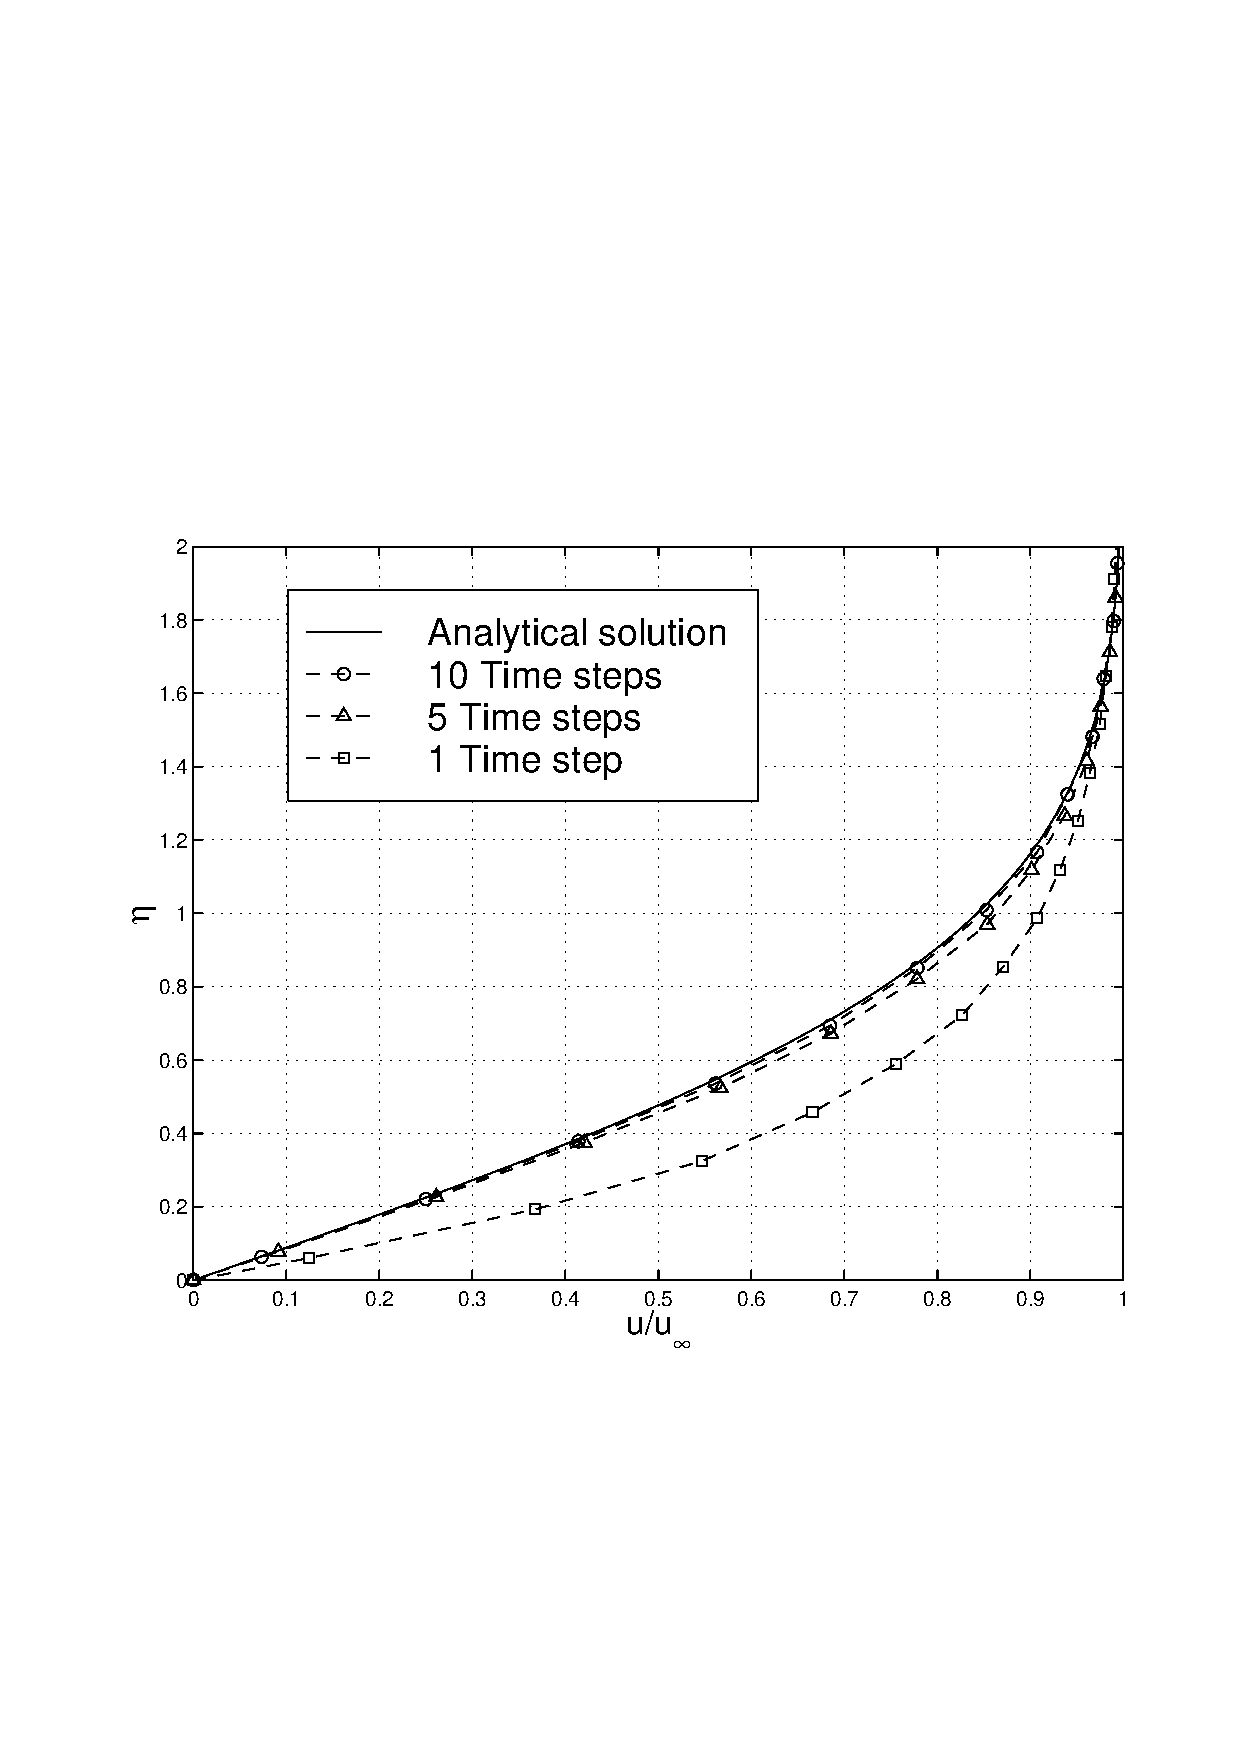
\includegraphics[width=110mm,clip=t]{CHAP_NONLIN/FIGURE/flat_sol.pdf}}
        \\
    \subfigure[Convergence history]
       {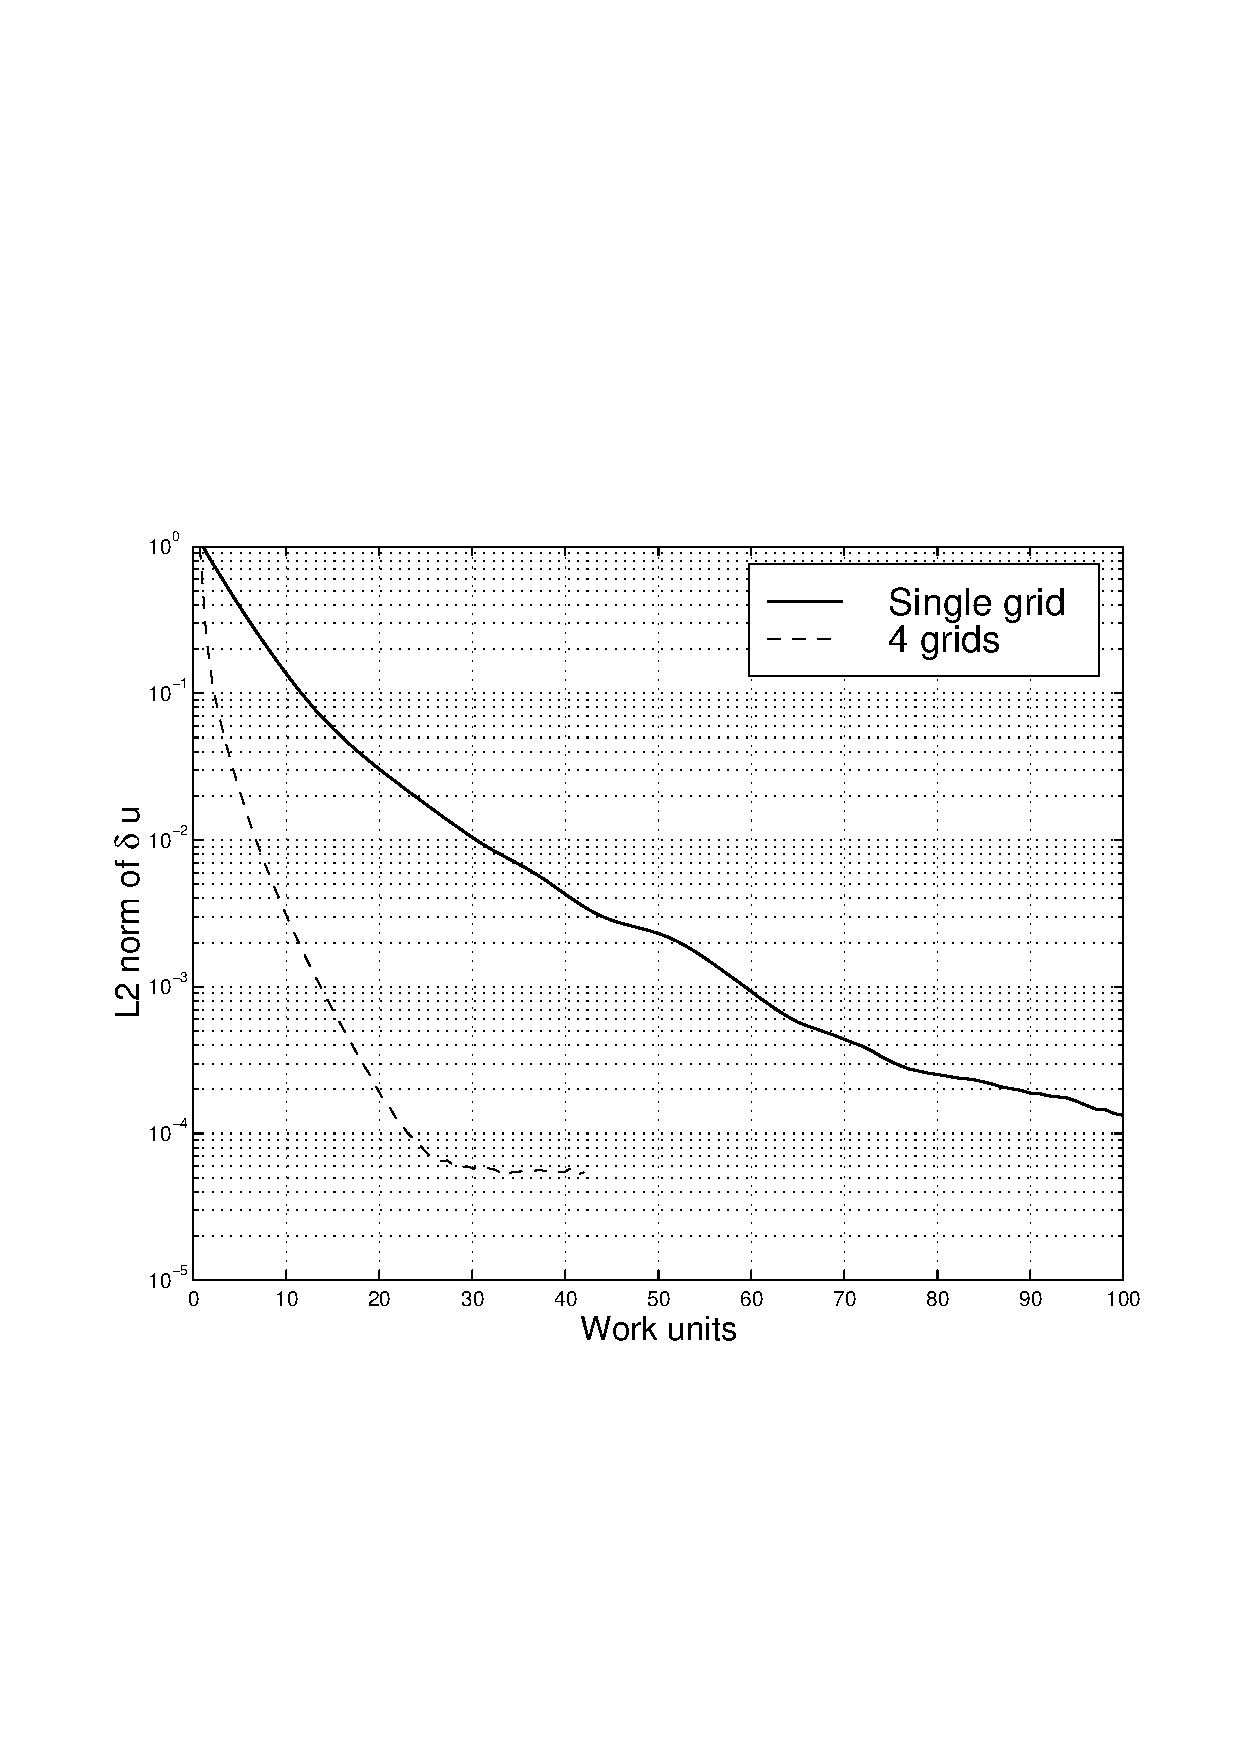
\includegraphics[width=110mm,clip=t]{CHAP_NONLIN/FIGURE/flat_res.pdf}}
  \end{tabular}
 \end{center}
 \vspace{-8mm}
 \caption{Impulsively started flat plate. $M_\infty = 0.2$, $Re_\infty = 40,000$.
          Velocity profiles and residual history}
 \label{flat_impul.fig}
\end{figure}

 Three calculations were performed with the present method with 1, 5 and 10
 physical time steps to reach the same physical time $t = 0.001\ sec$.
 The maximum ratio between the physical and pseudo time step, $\Delta t/\Delta\tau$,
 was of around 17,000 for the case where a single time step was used to reached
 $t = 0.001\ sec$. Fig. \ref{flat_impul.fig}a shows the comparison between
 the numerical and analytical solutions. As expected, the smaller the physical time
 step, the better the agreement.
 If one used an explicit method to calculate the unsteady flow at the same physical
 time level, than it should have performed around 15,000 time steps using
 a CFL number of 1.5. For the case of 5 time step the convergence of
 (\ref{Dual_time_stepping_3.eq}) for a given time level was obtained with $\approx 15$
 W multigrid cycles using four grids. In terms of CPU time this means
 that with 5 time steps the present method was $\approx 120$ times faster than
 an explicit Runge-Kutta integration method.

 Fig. \ref{flat_impul.fig}b shows the comparison of the
 residual within a given physical time step, using a single grid and a four grids
 W-type cycle. As one would expected, the convergece to a new physical time level
 improves if more the one grid are used. However such improvement does not
 compare with the one obtained for steady-state computations.
 Convergence histories similar to the one
 shown in Fig. \ref{flat_impul.fig}b represents the best result
 obtained for unsteady flows.

%
%
%
%
\subsection{Vortex shedding past a cylinder}
\label{vortex_shedding_cylinder.subsec}
%
\begin{figure}
 \begin{center}
  \begin{tabular}{cc}
    \subfigure[Computational grid: 17391 points]
        {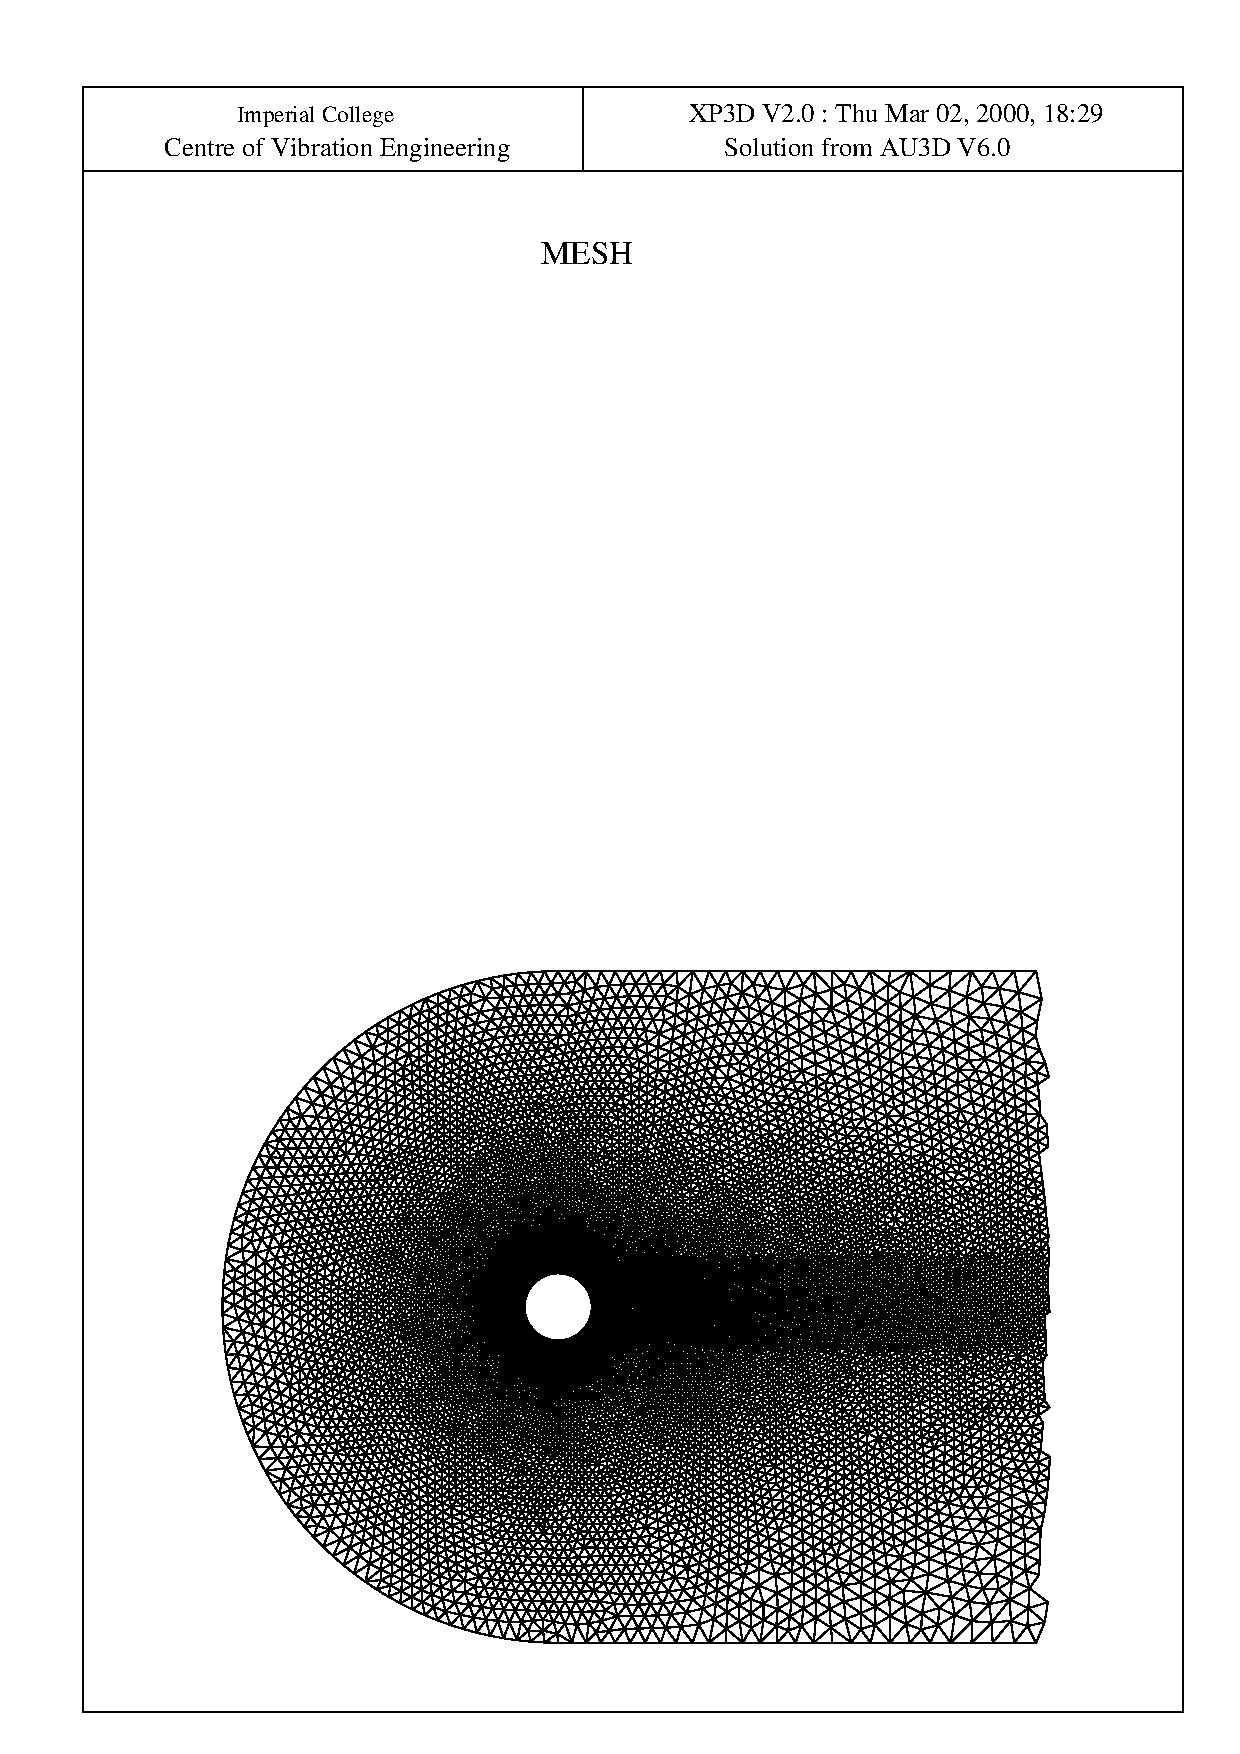
\includegraphics[height=60mm,clip=t]{CHAP_NONLIN/FIGURE/cil_me1.pdf}}
        &
    \subfigure[Zoom view at leading edge]
        {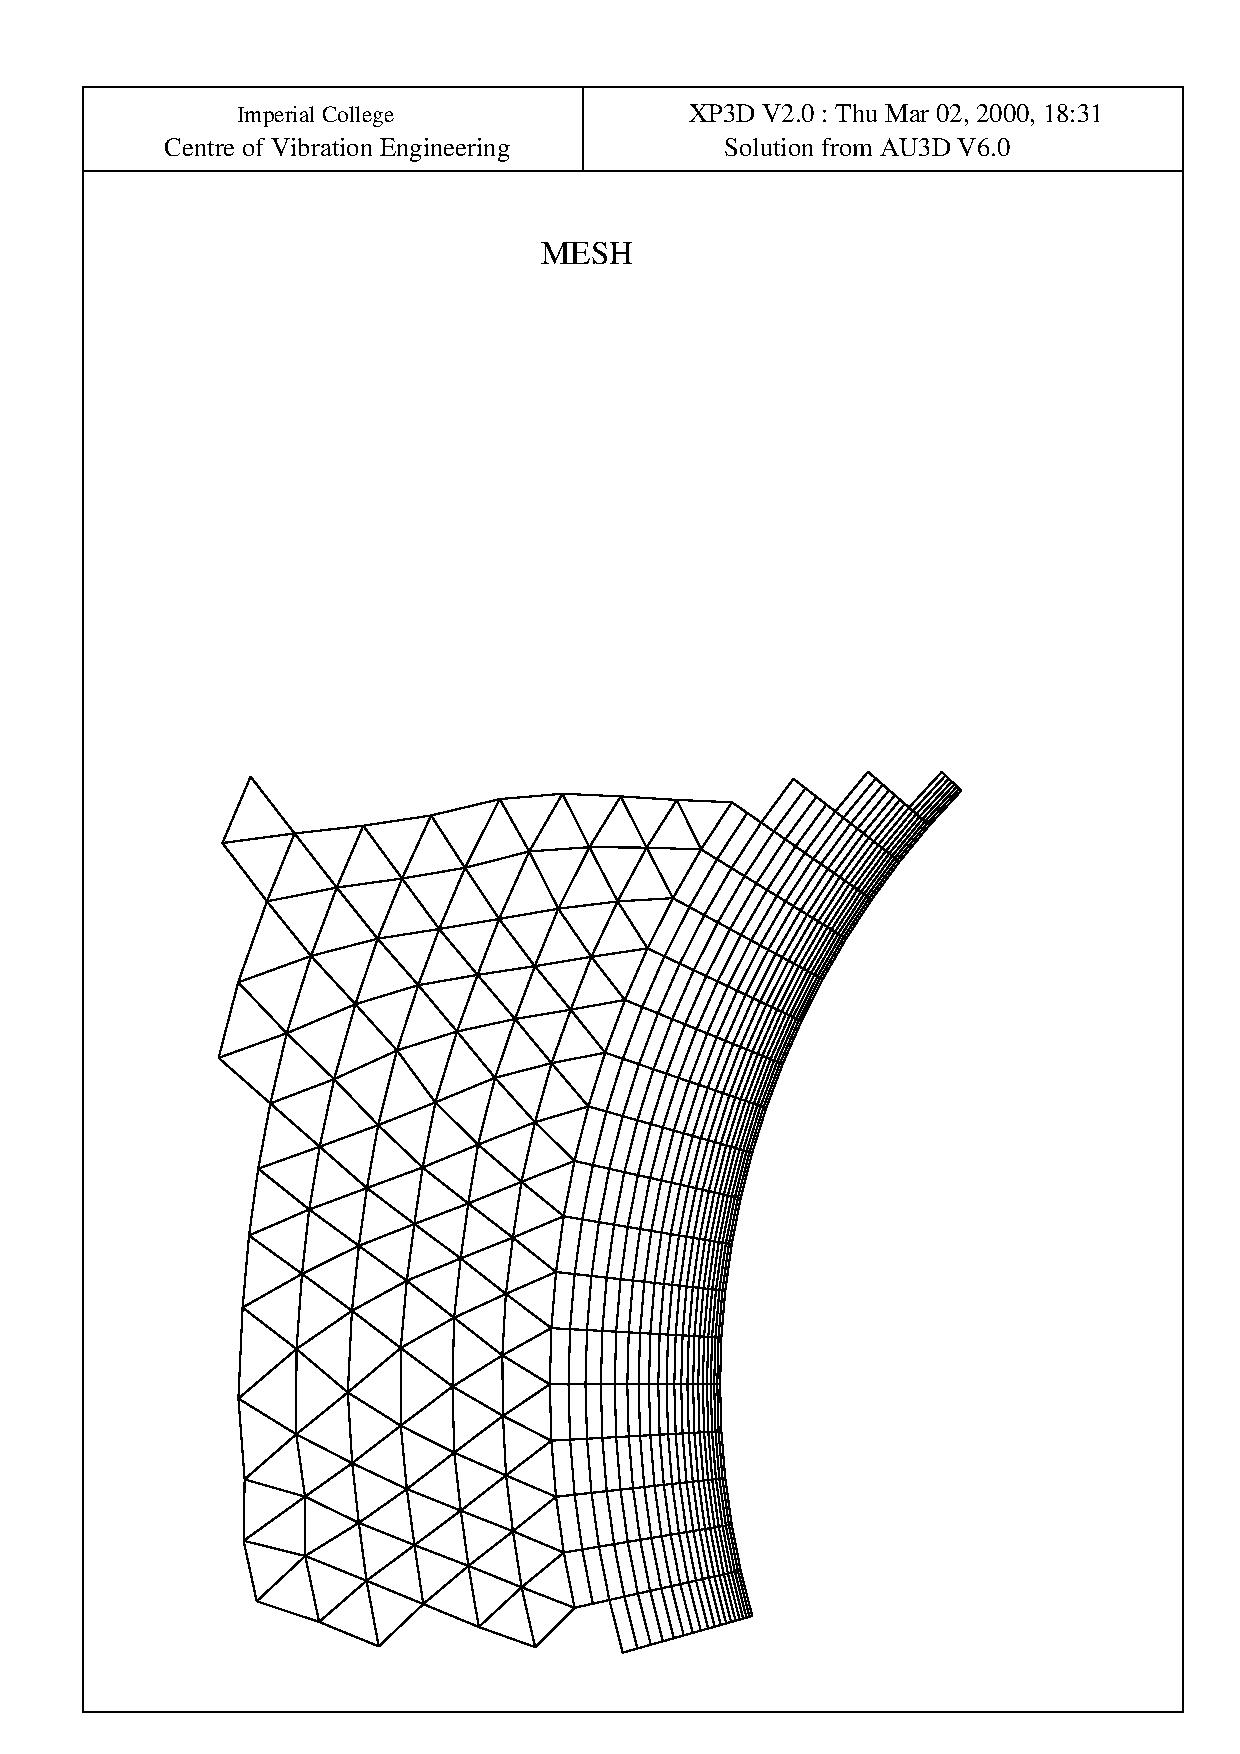
\includegraphics[height=60mm,clip=t]{CHAP_NONLIN/FIGURE/cil_me0.pdf}}
  \end{tabular}
 \end{center}
 \vspace{-5mm}
 \caption{Circular cylinder. Computational mesh}
 \label{cil_mesh1.fig}
\end{figure}
%
 This test case is intended to predict the natural vortex shedding
 past a cylinder in a laminar incompressible flow regime.
 Vortex shedding is one of many viscous flows which, though posed
 with fixed and steady boundary conditions, evolve into unsteady
 motions because of flow instability.
 If one consider a circular cylinder with diameter $d$, then
 the incompressible flow field generated by a uniform
 velocity at infinity $u_\infty$
 is dependent solely upon the Reynolds number $Re_d$

%
\beq
  Re_d = \frac{\rho_\infty u_\infty d}{\mu_\infty}
\eeq
%
 If $Re_d < 40$ the flow is steady. If $Re_d > 40$
 the flow becomes unstable and consequently unsteady when
 $Re_d > 50$. The flow field is caracterised by a unsteady wake
 which consists of pairs of vortices shed alternately from the
 upper and lower part of the cylinder surface.
 If $50 < Re_d < 150$ such a wake structure is well organised and is
 called Karman vortex sheet after a paper by Karman (1911) explaining
 this alternation to be a stable configuration for vortex pairs
 (Schlichting \citeyearNP{Schlichting}).
 An important feature of this flow is that the dimensionless
 cylinder frequency or Stroudal number

%
\beq
  St = \frac{f d}{u_\infty}
\eeq
%
 remains constant $\approx 0.21$ for $100 < Re_d < 10,000$. Thus, in this
 Reynolds number range, the shedding cycle takes place during the time
 that the free-stream moves approximately five cylinder diameters.
%
\begin{figure}[ht]
 \begin{center}
  \begin{tabular}{ccc}
    \subfigure[Grid 2: 4308 cells]
       {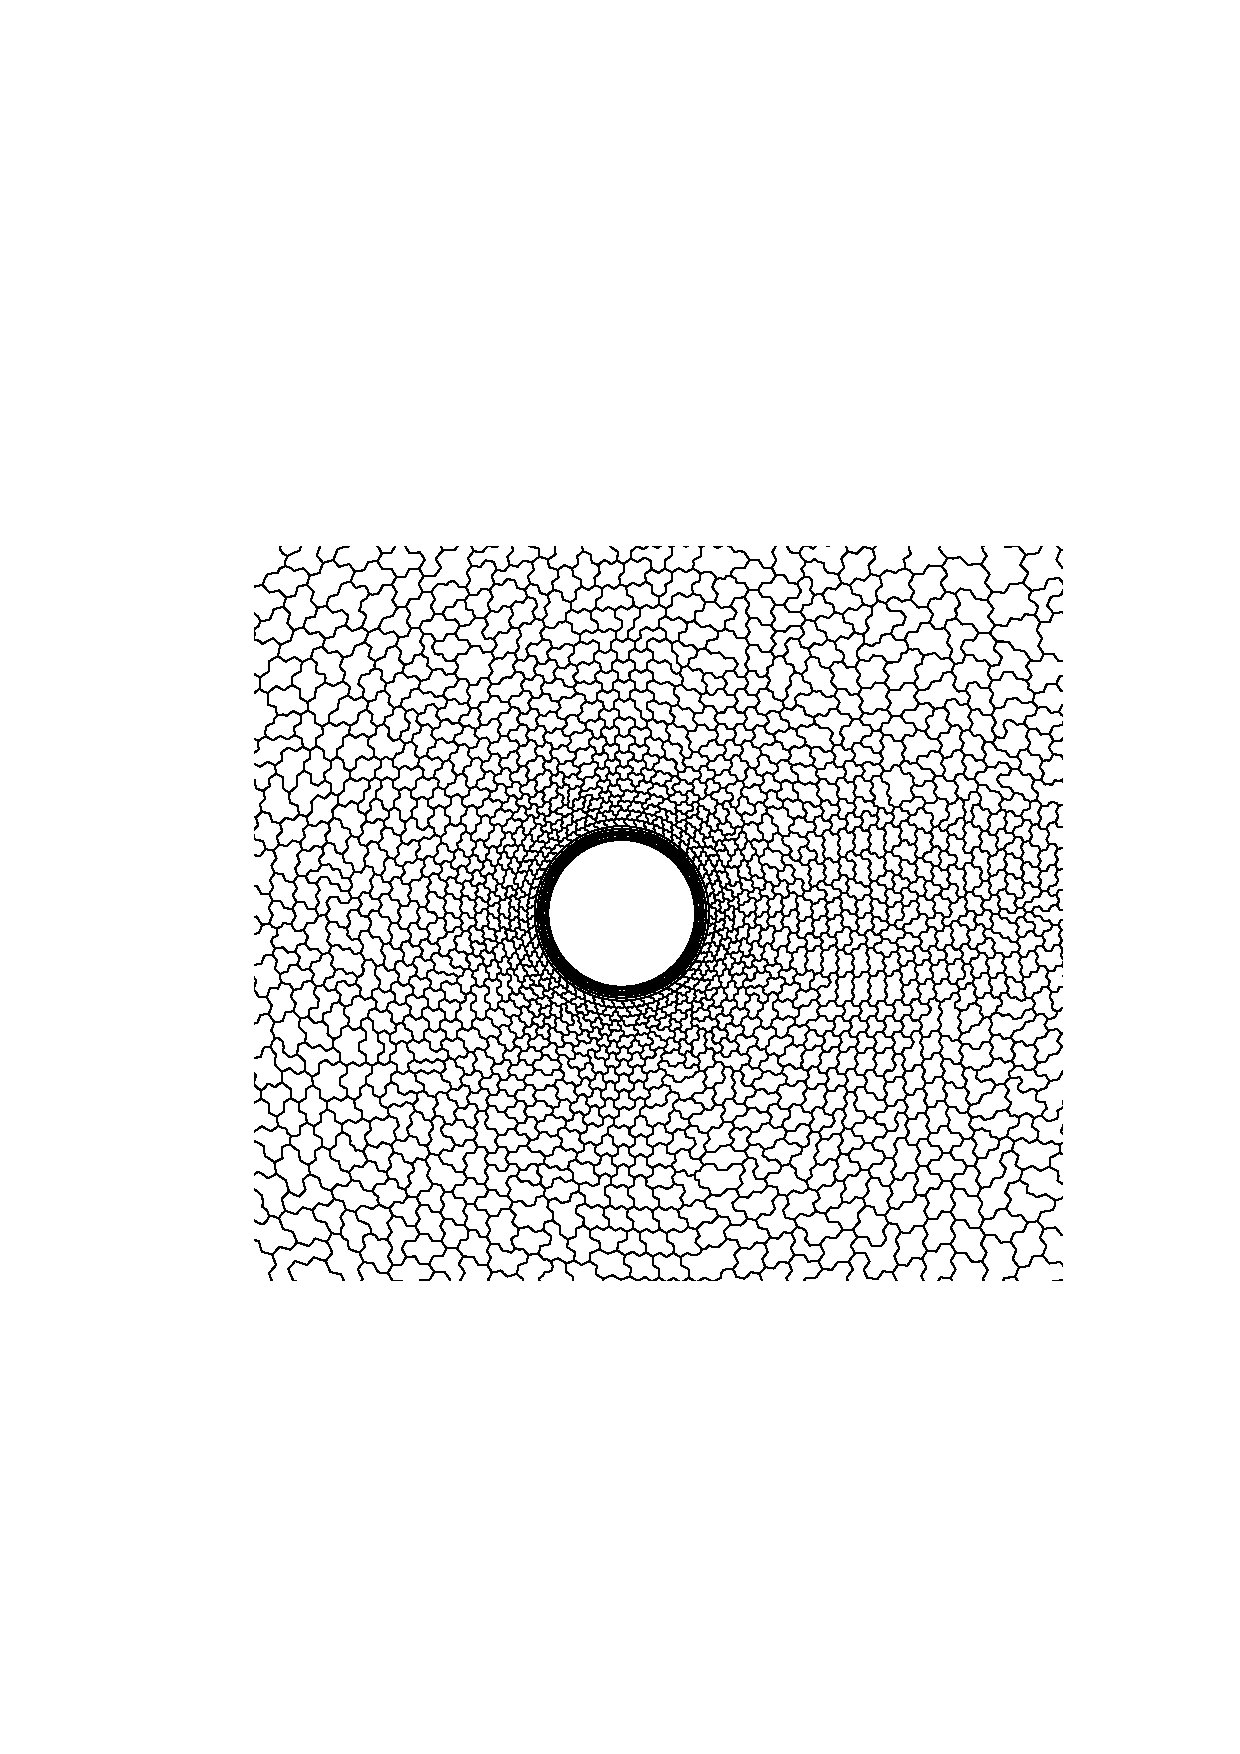
\includegraphics[width=45mm,clip=t]{CHAP_NONLIN/FIGURE/cil_me2.pdf}}
        &
    \subfigure[Grid 3: 1095 cells]
       {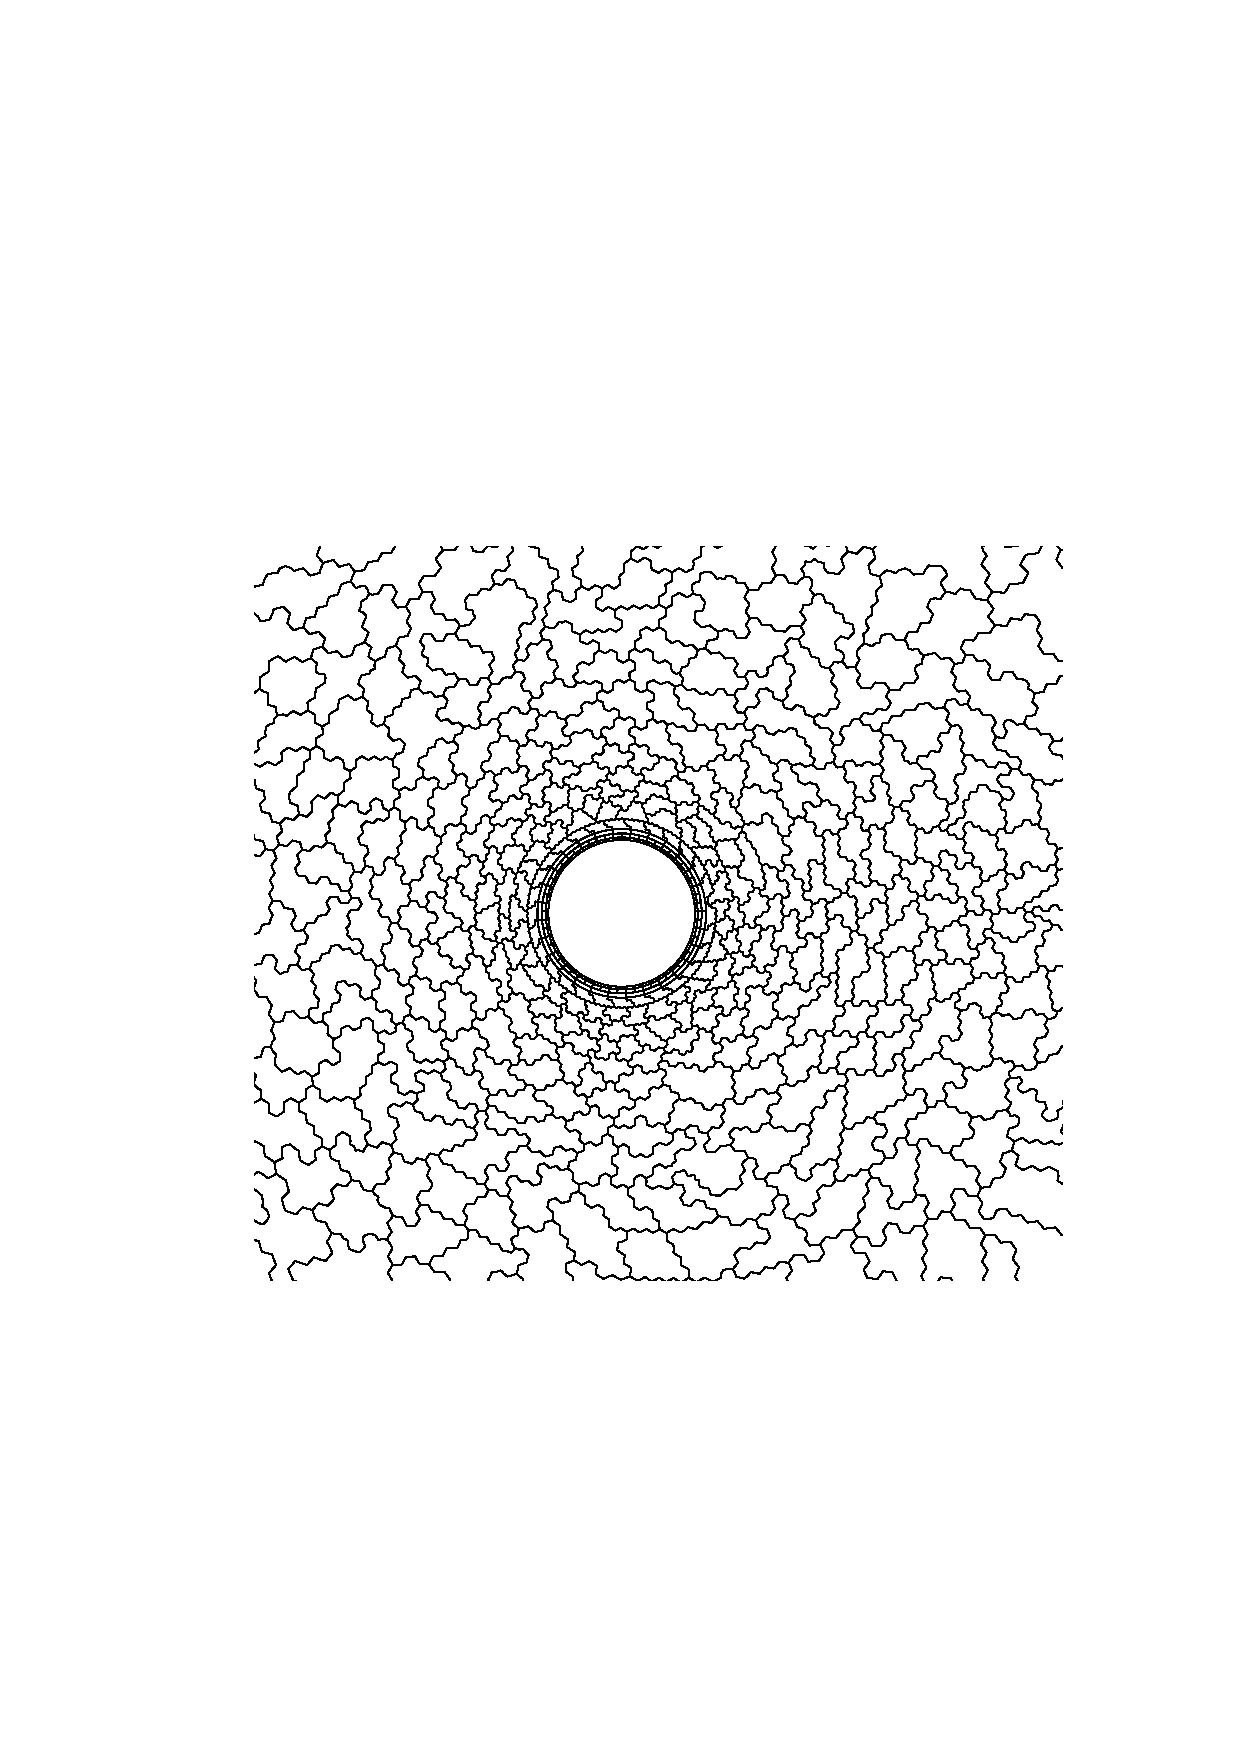
\includegraphics[width=45mm,clip=t]{CHAP_NONLIN/FIGURE/cil_me3.pdf}}
        &
    \subfigure[Grid 4: 283 cells]
       {\includegraphics[width=45mm,clip=t]{CHAP_NONLIN/FIGURE/cil_me4.pdf}}
  \end{tabular}
 \end{center}
 \vspace{-5mm}
 \caption{Circular cylinder. Agglomerated grids}
 \label{cil_mesh2.fig}
\end{figure}

 Fig. \ref{cil_mesh1.fig} shows the computational mesh used for this test case,
 it contains 2280 quadrilaterals in the boundary layer and 29863
 triangles in the rest of the domain for a total number of point of 17391.
 Fig. \ref{cil_mesh2.fig} shows the three agglomerated grids used in the time
 accurate multigrid algorithm.
 Four different calculations were performed for various Reynolds numbers
 with an inlet Mach number of 0.2
 and the computed Stroudal number is reported in Fig. \ref{stroudal.fig}a together
 with the experimental value of 0.21. The comparison is satisfactory for
 all four test cases.
 Fig. \ref{stroudal.fig}b reports the evolution in time of the pressure coefficient
 at a point in the wake close to the cylinder. The time history refers to three cycles of
 oscillations after a periodic flow conditions is reached. The very periodic behaviour
 of the flow is evident and proves the robustness and accuracy of the scheme.
%
\begin{figure}
 \begin{center}
  \begin{tabular}{c}
    \subfigure[Computed Stroudal number]
       {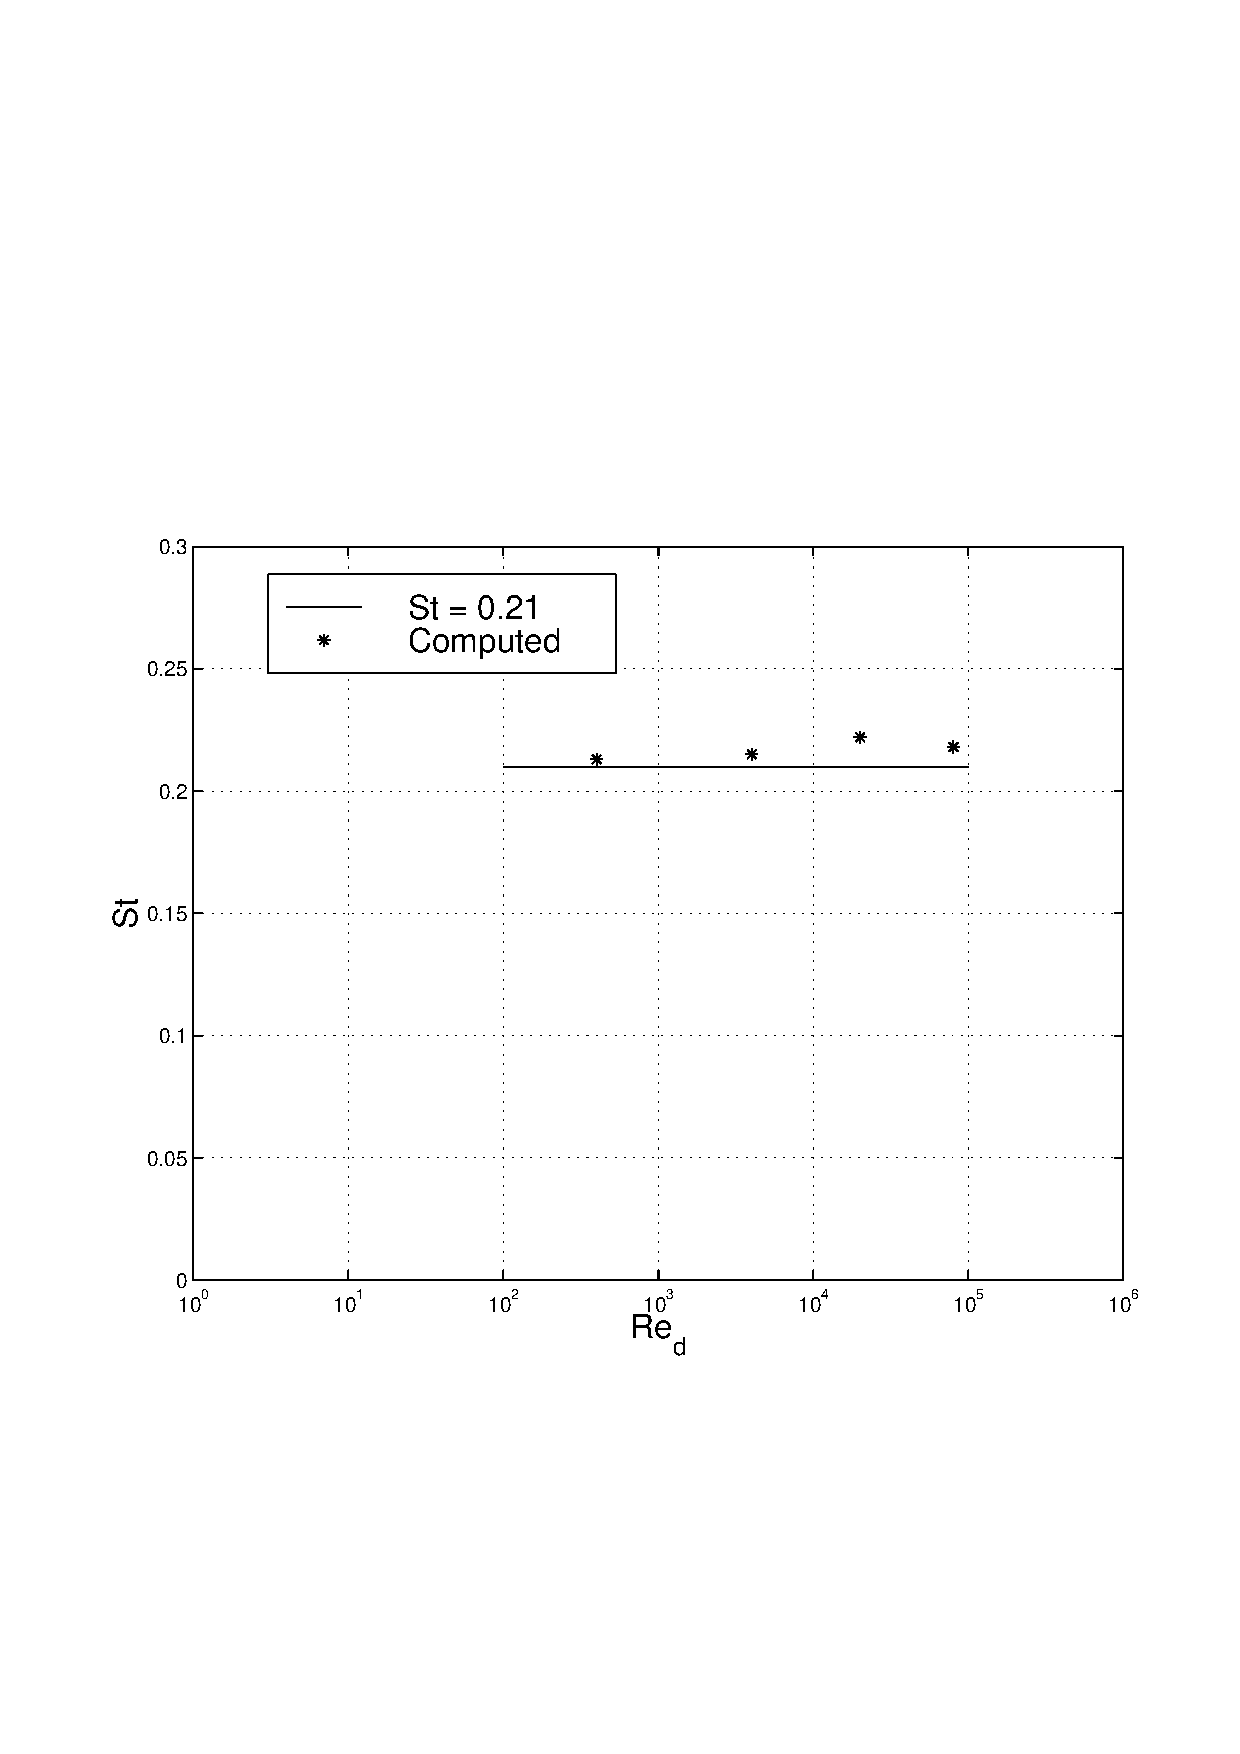
\includegraphics[width=110mm,clip=t]{CHAP_NONLIN/FIGURE/stroud.pdf}}
        \\
    \subfigure[$c_p$ evolution]
       {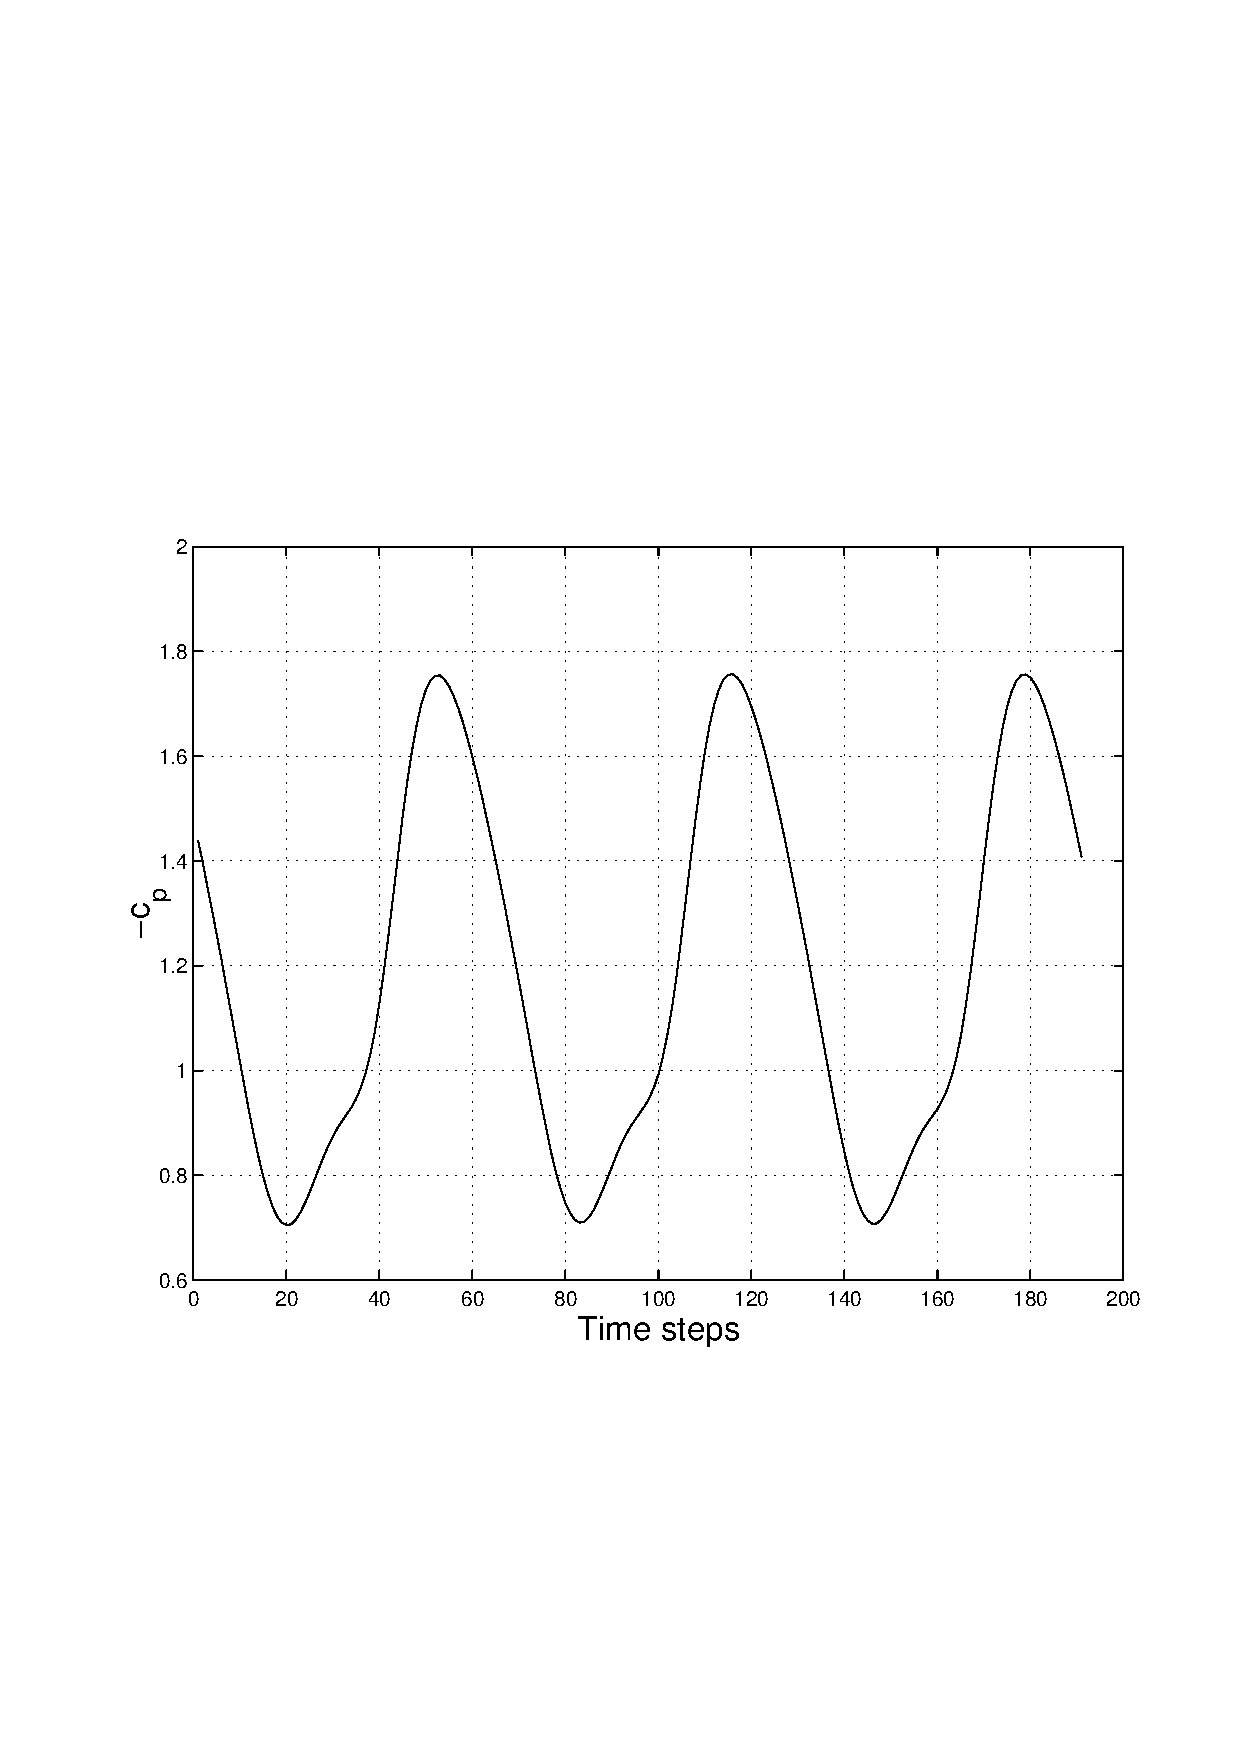
\includegraphics[width=110mm,clip=t]{CHAP_NONLIN/FIGURE/prehis.pdf}}
  \end{tabular}
 \end{center}
 \vspace{-5mm}
 \caption{Circular cylinder. Computed Stroudal number and $c_p$ evolution}
 \label{stroudal.fig}
\end{figure}
%

 The time step for those calculations was set to have 50 divisions over a cycle.
 This correspond to a local CFL number between two in the far field and three
 thousand in the boundary layer region.
%
\begin{figure}[ht]
 \begin{center}
  \begin{tabular}{c}
    \subfigure[$Re_d = 400$]
       {\begin{tabular}{ccc}
         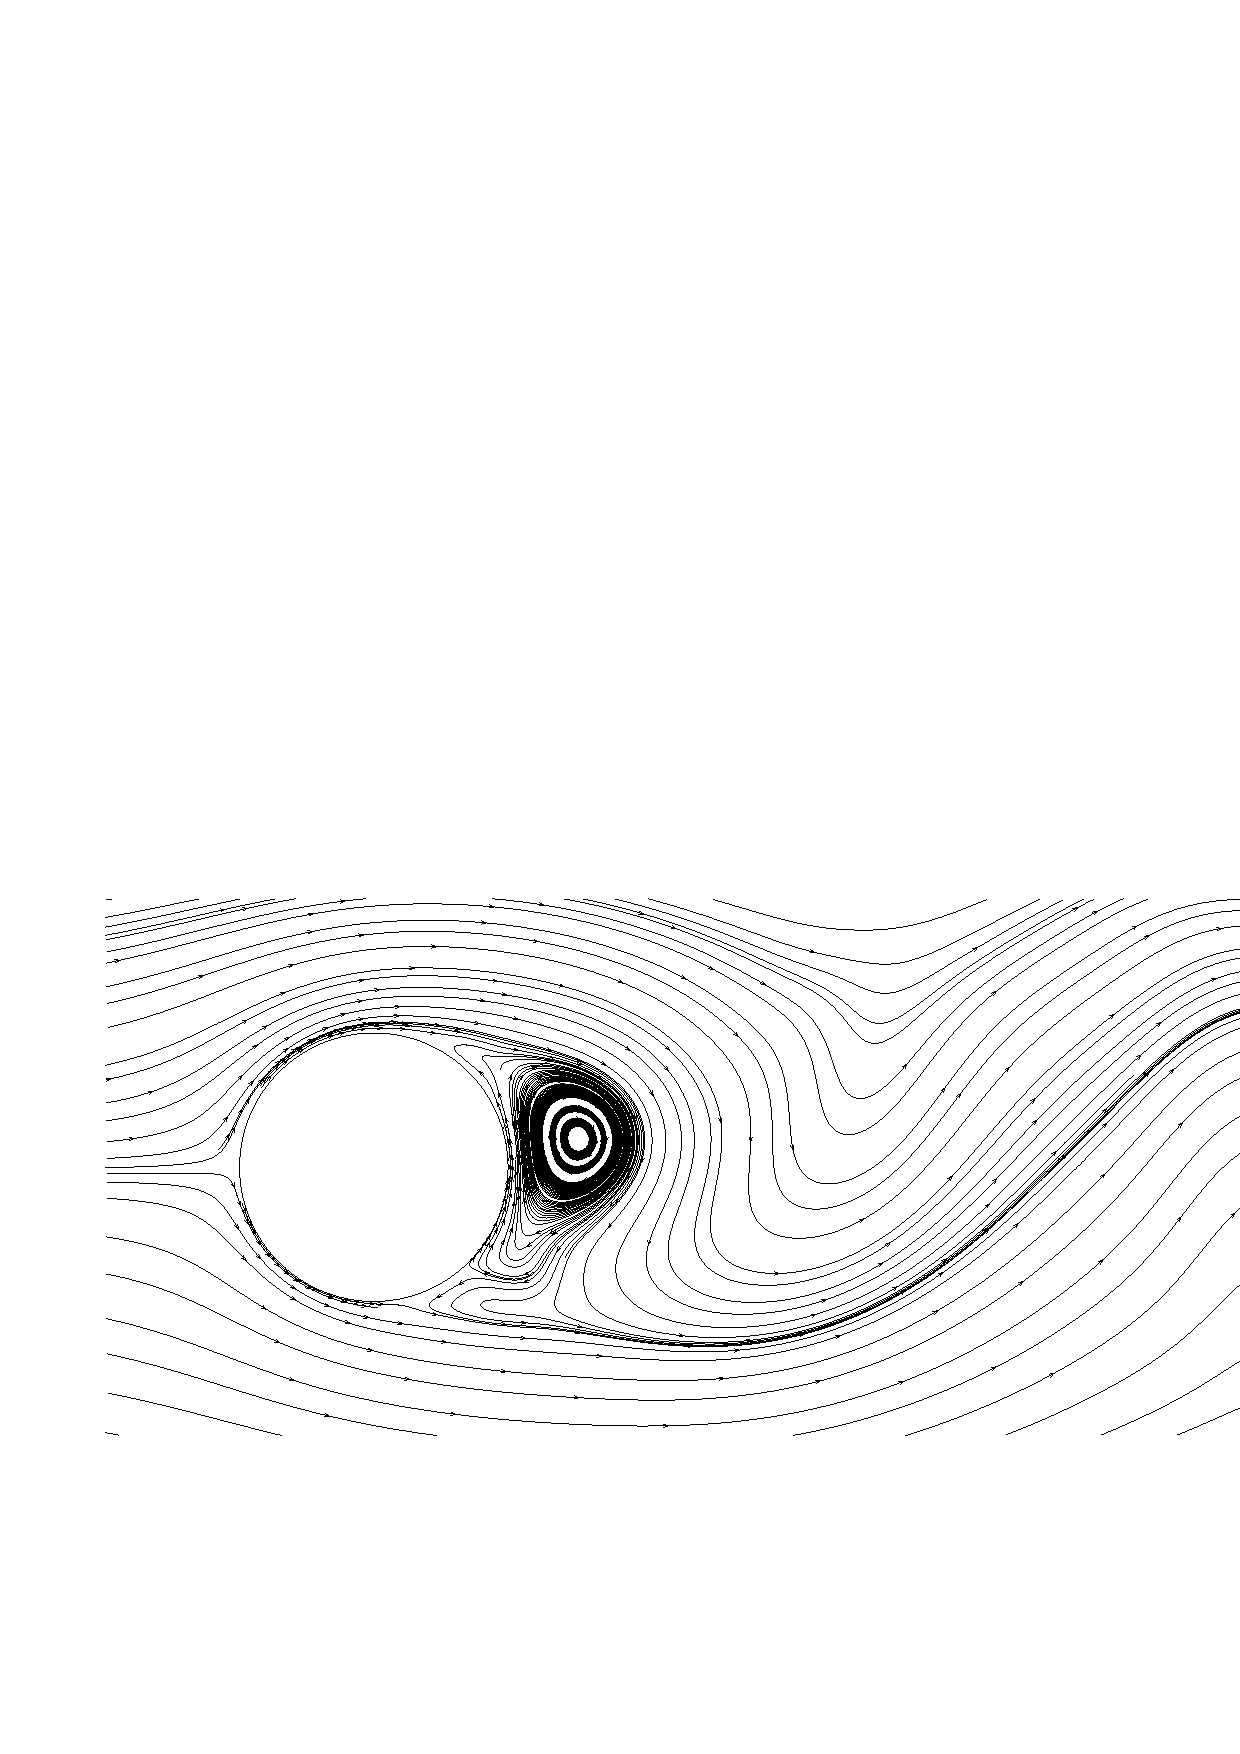
\includegraphics[width=45mm,clip=t]{CHAP_NONLIN/FIGURE/cil2.pdf}
         &
         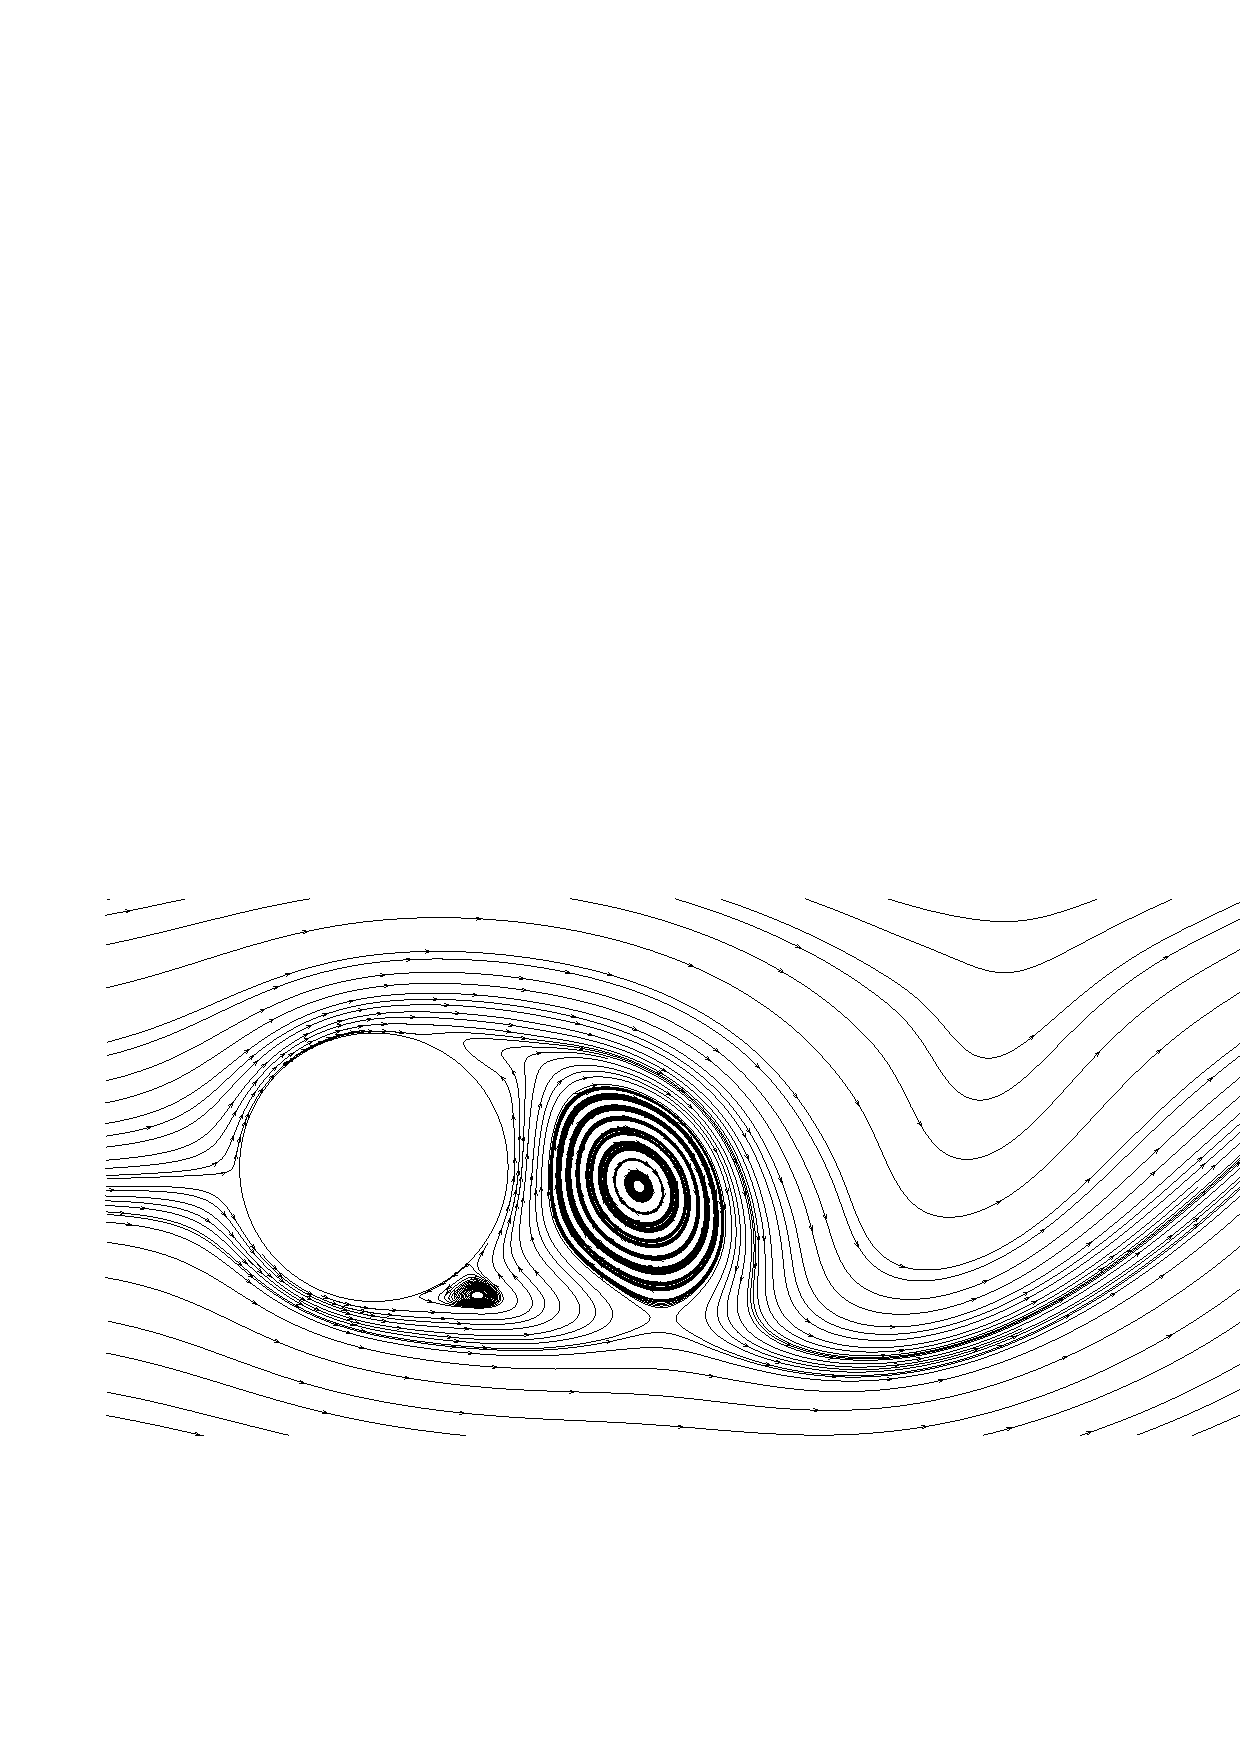
\includegraphics[width=45mm,clip=t]{CHAP_NONLIN/FIGURE/cil3.pdf}
         &
         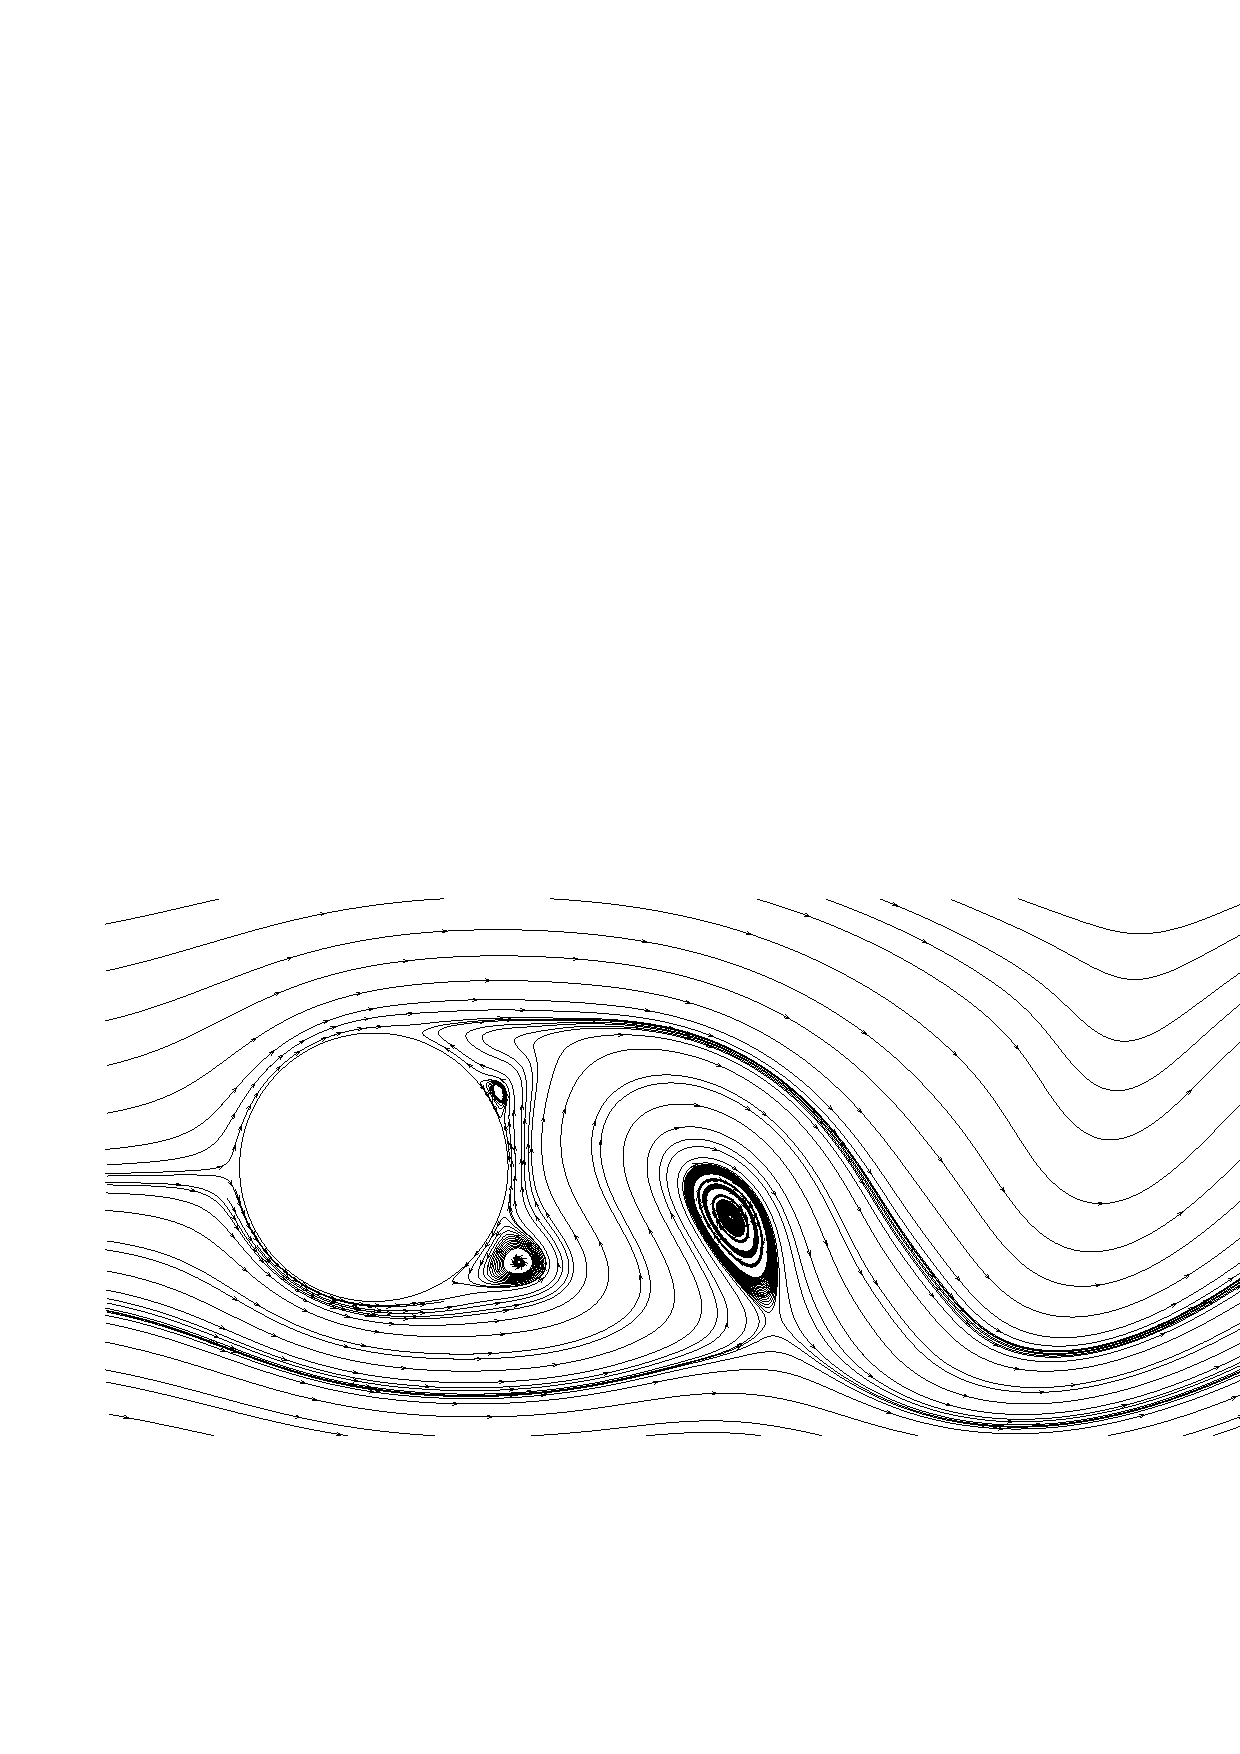
\includegraphics[width=45mm,clip=t]{CHAP_NONLIN/FIGURE/cil4.pdf}
        \\
         Time 1 & Time 2 & Time 3
        \\
         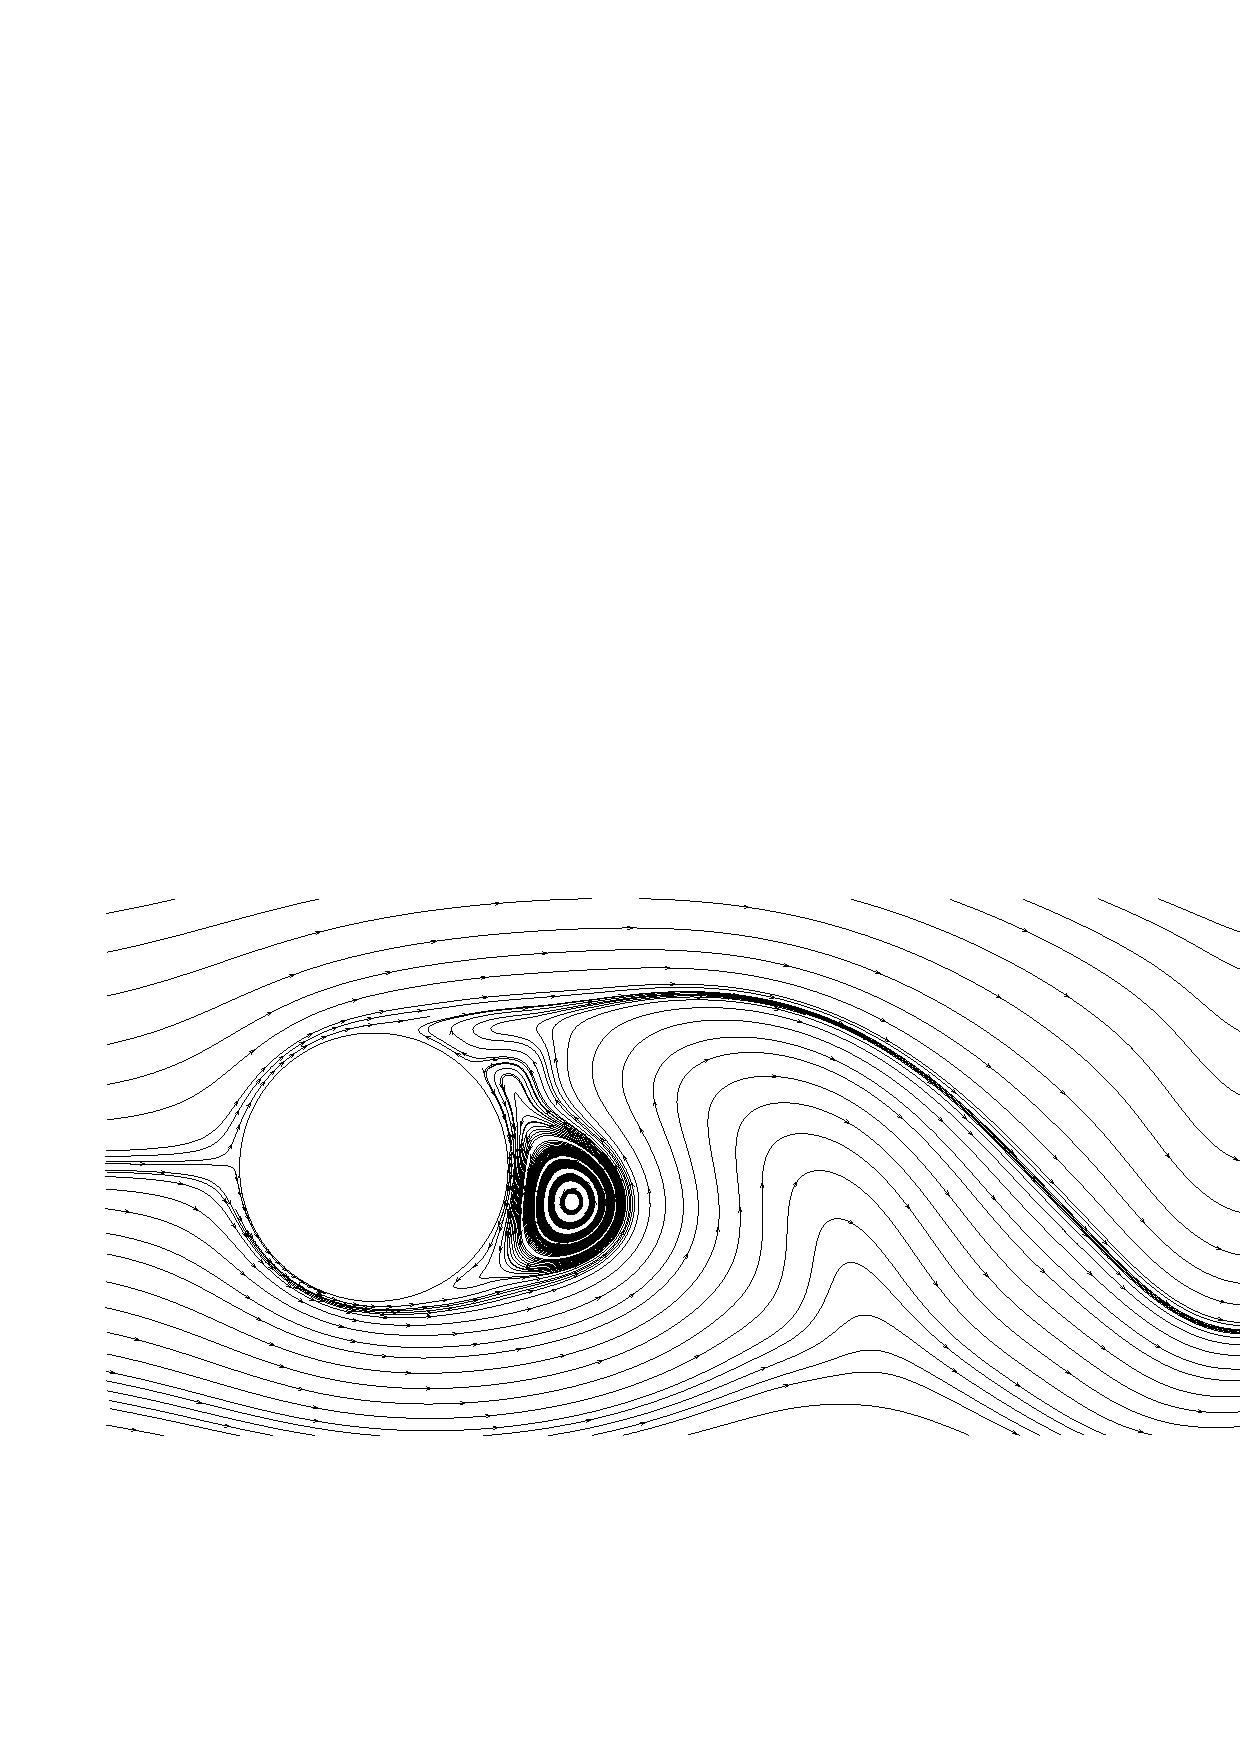
\includegraphics[width=45mm,clip=t]{CHAP_NONLIN/FIGURE/cil5.pdf}
         &
         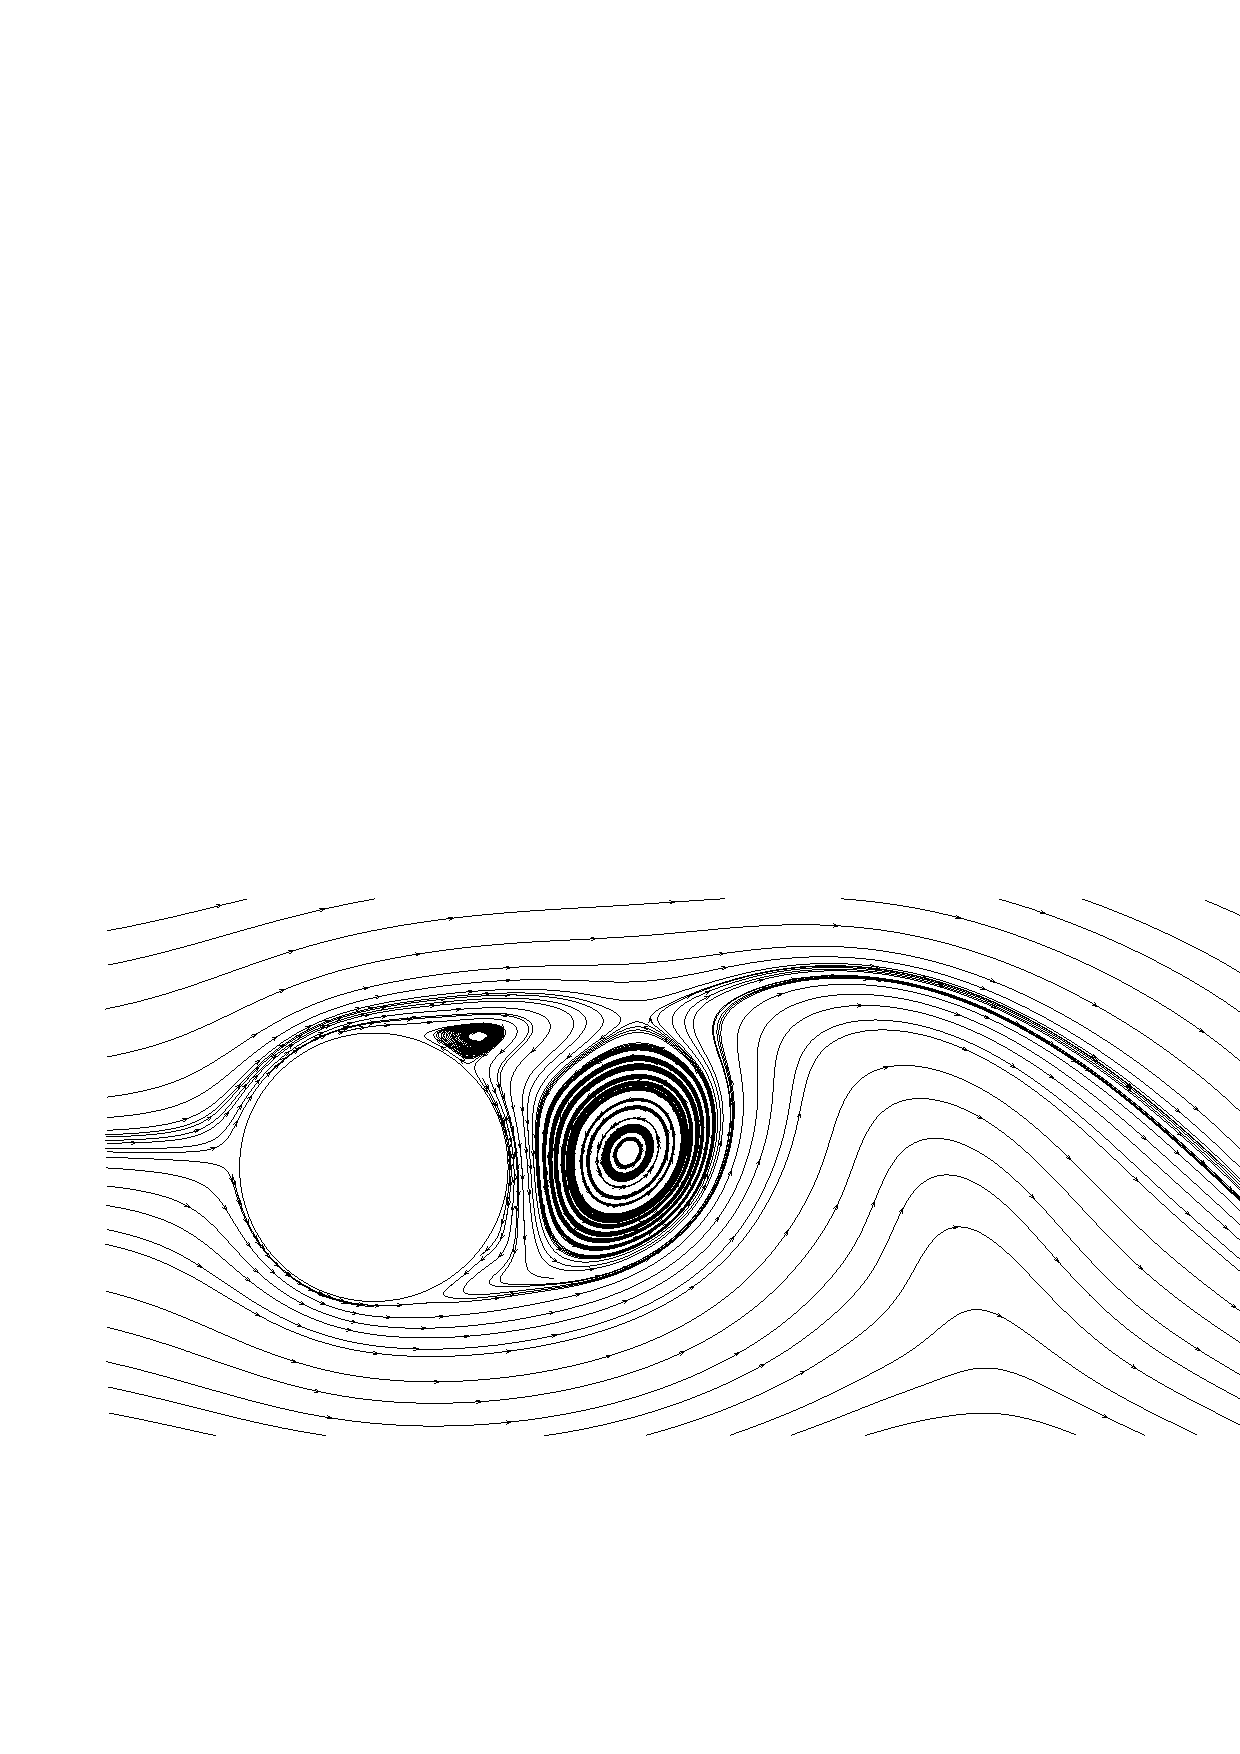
\includegraphics[width=45mm,clip=t]{CHAP_NONLIN/FIGURE/cil6.pdf}
         &
         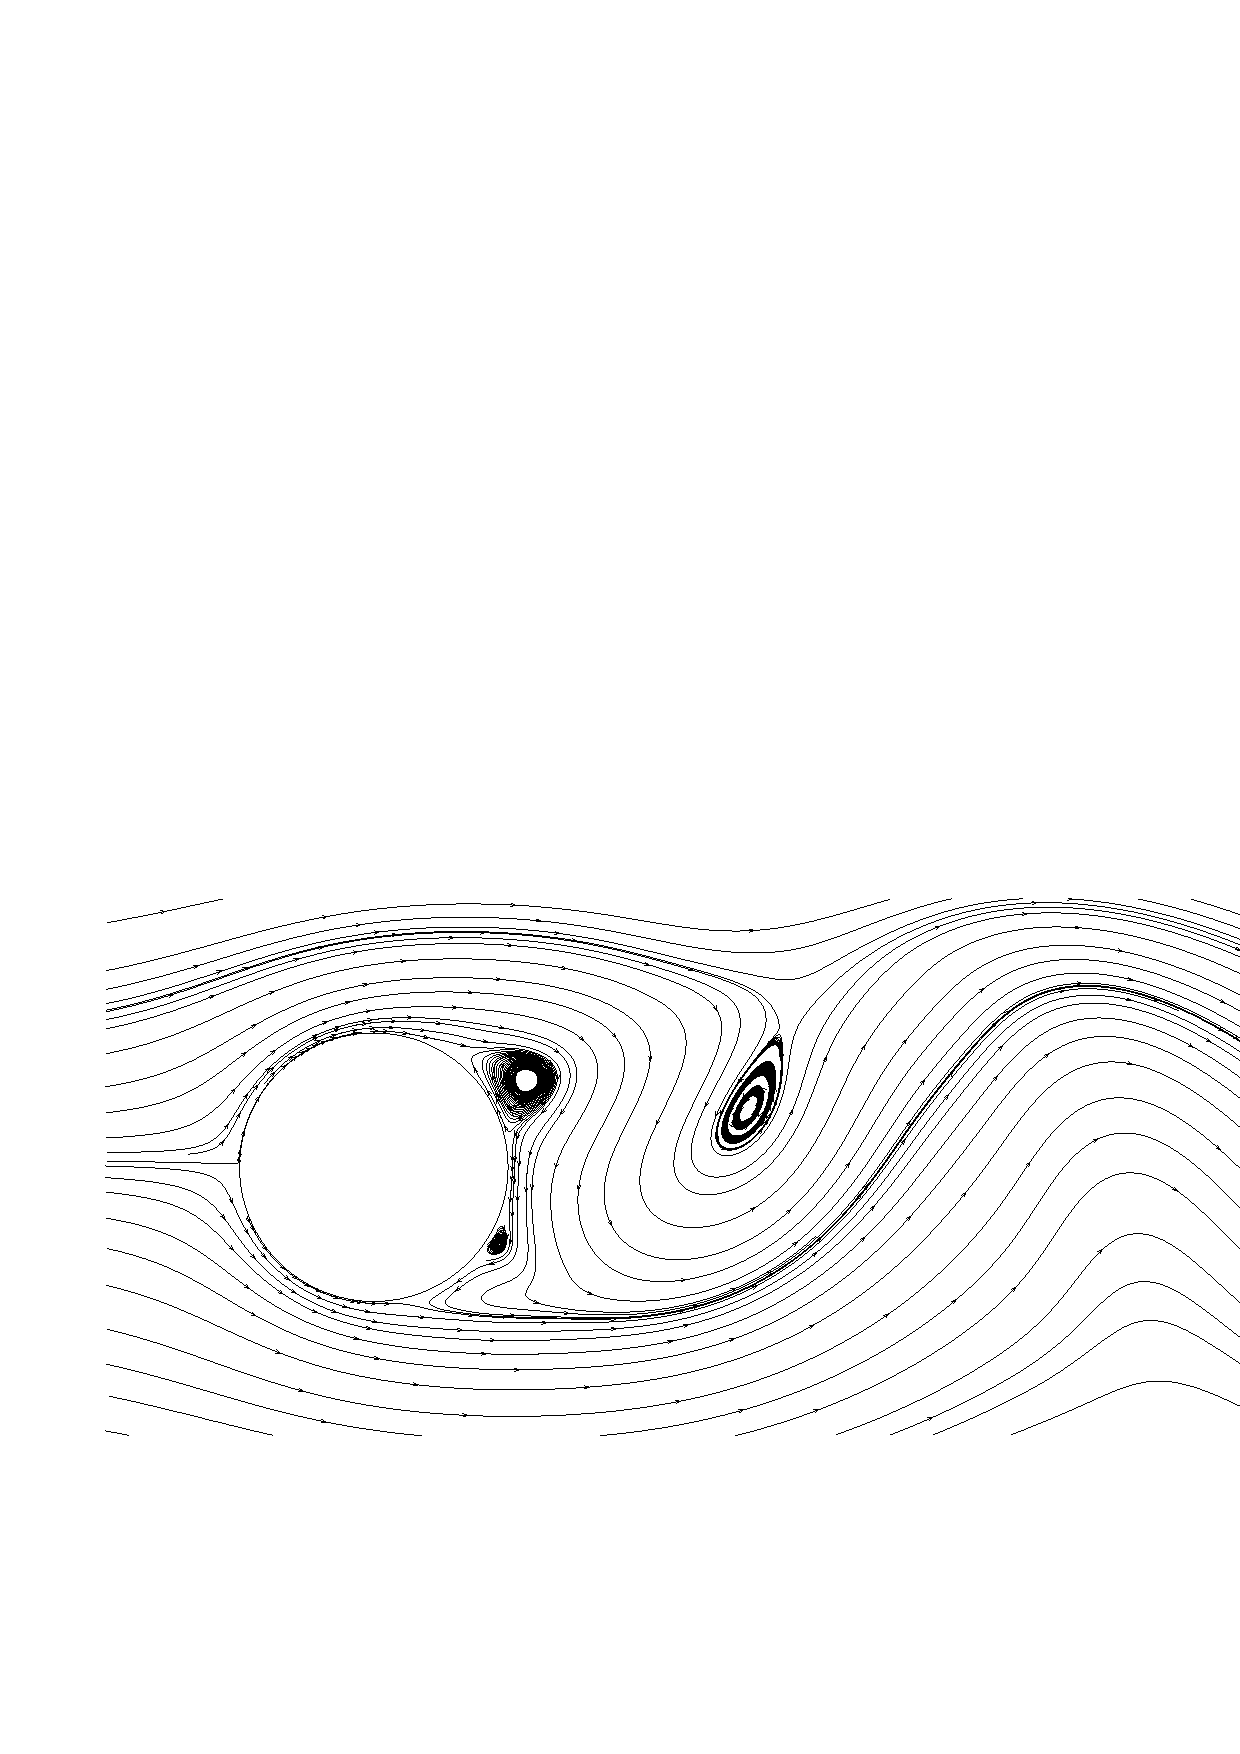
\includegraphics[width=45mm,clip=t]{CHAP_NONLIN/FIGURE/cil1.pdf}
        \\
         Time 4 & Time 5 & Time 6
       \end{tabular}}
     \\
    \subfigure[$Re_d = 4000$]
       {\begin{tabular}{ccc}
         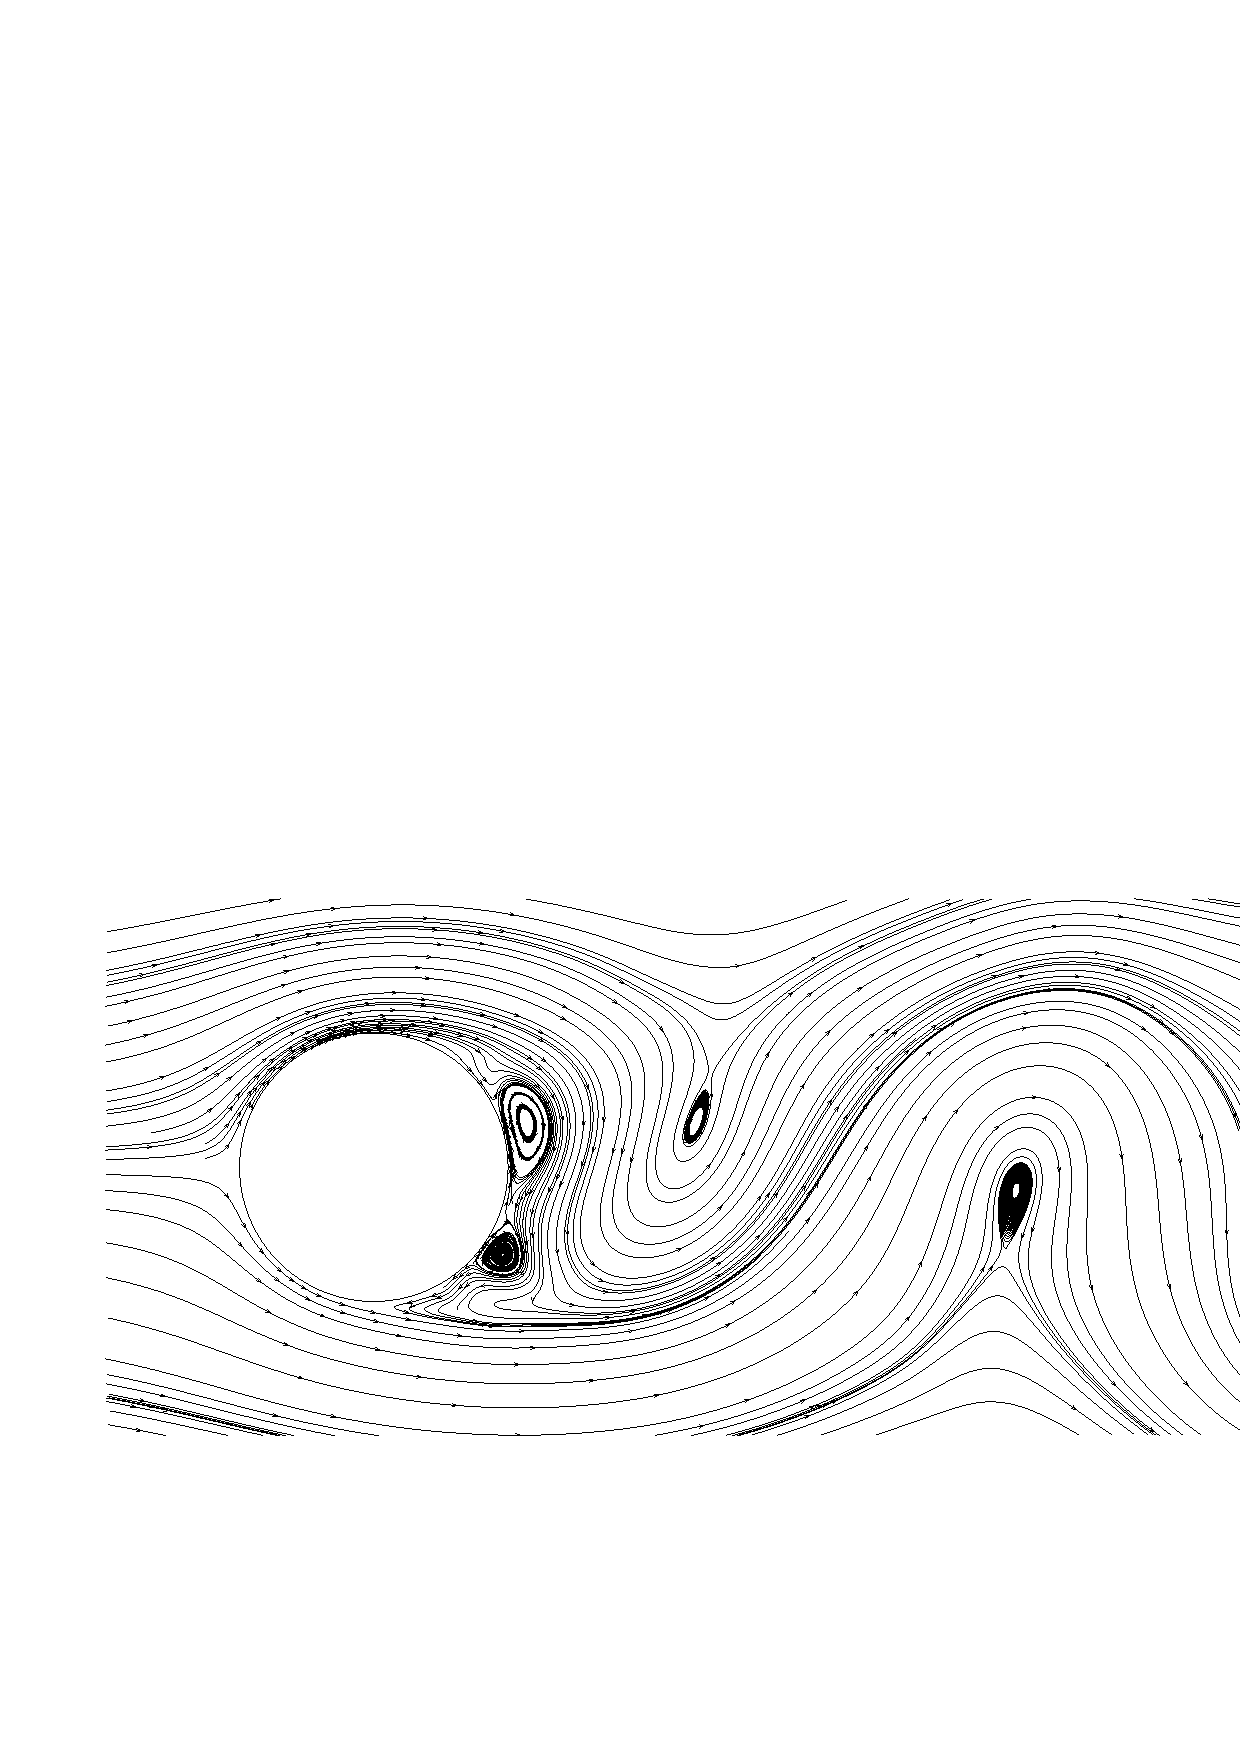
\includegraphics[width=45mm,clip=t]{CHAP_NONLIN/FIGURE/cim2.pdf}
         &
         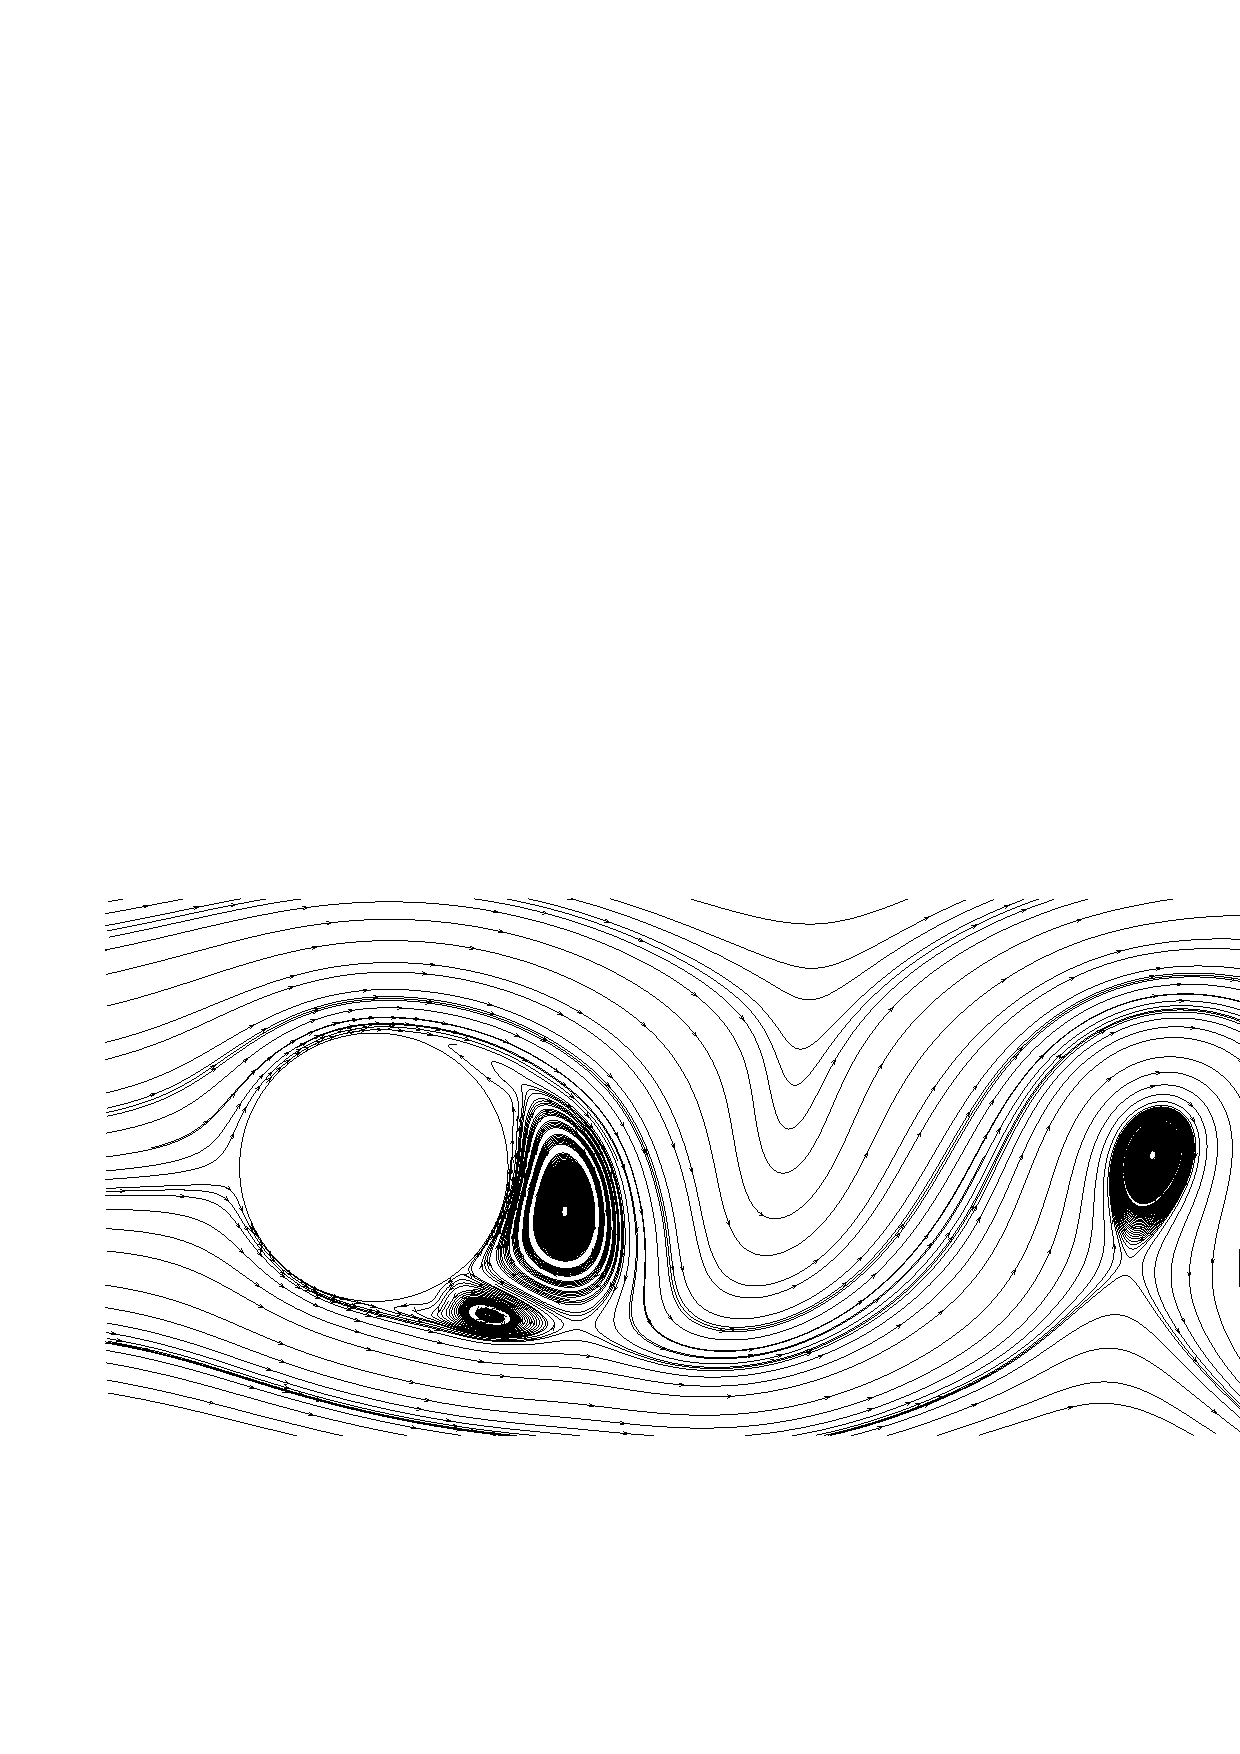
\includegraphics[width=45mm,clip=t]{CHAP_NONLIN/FIGURE/cim3.pdf}
         &
         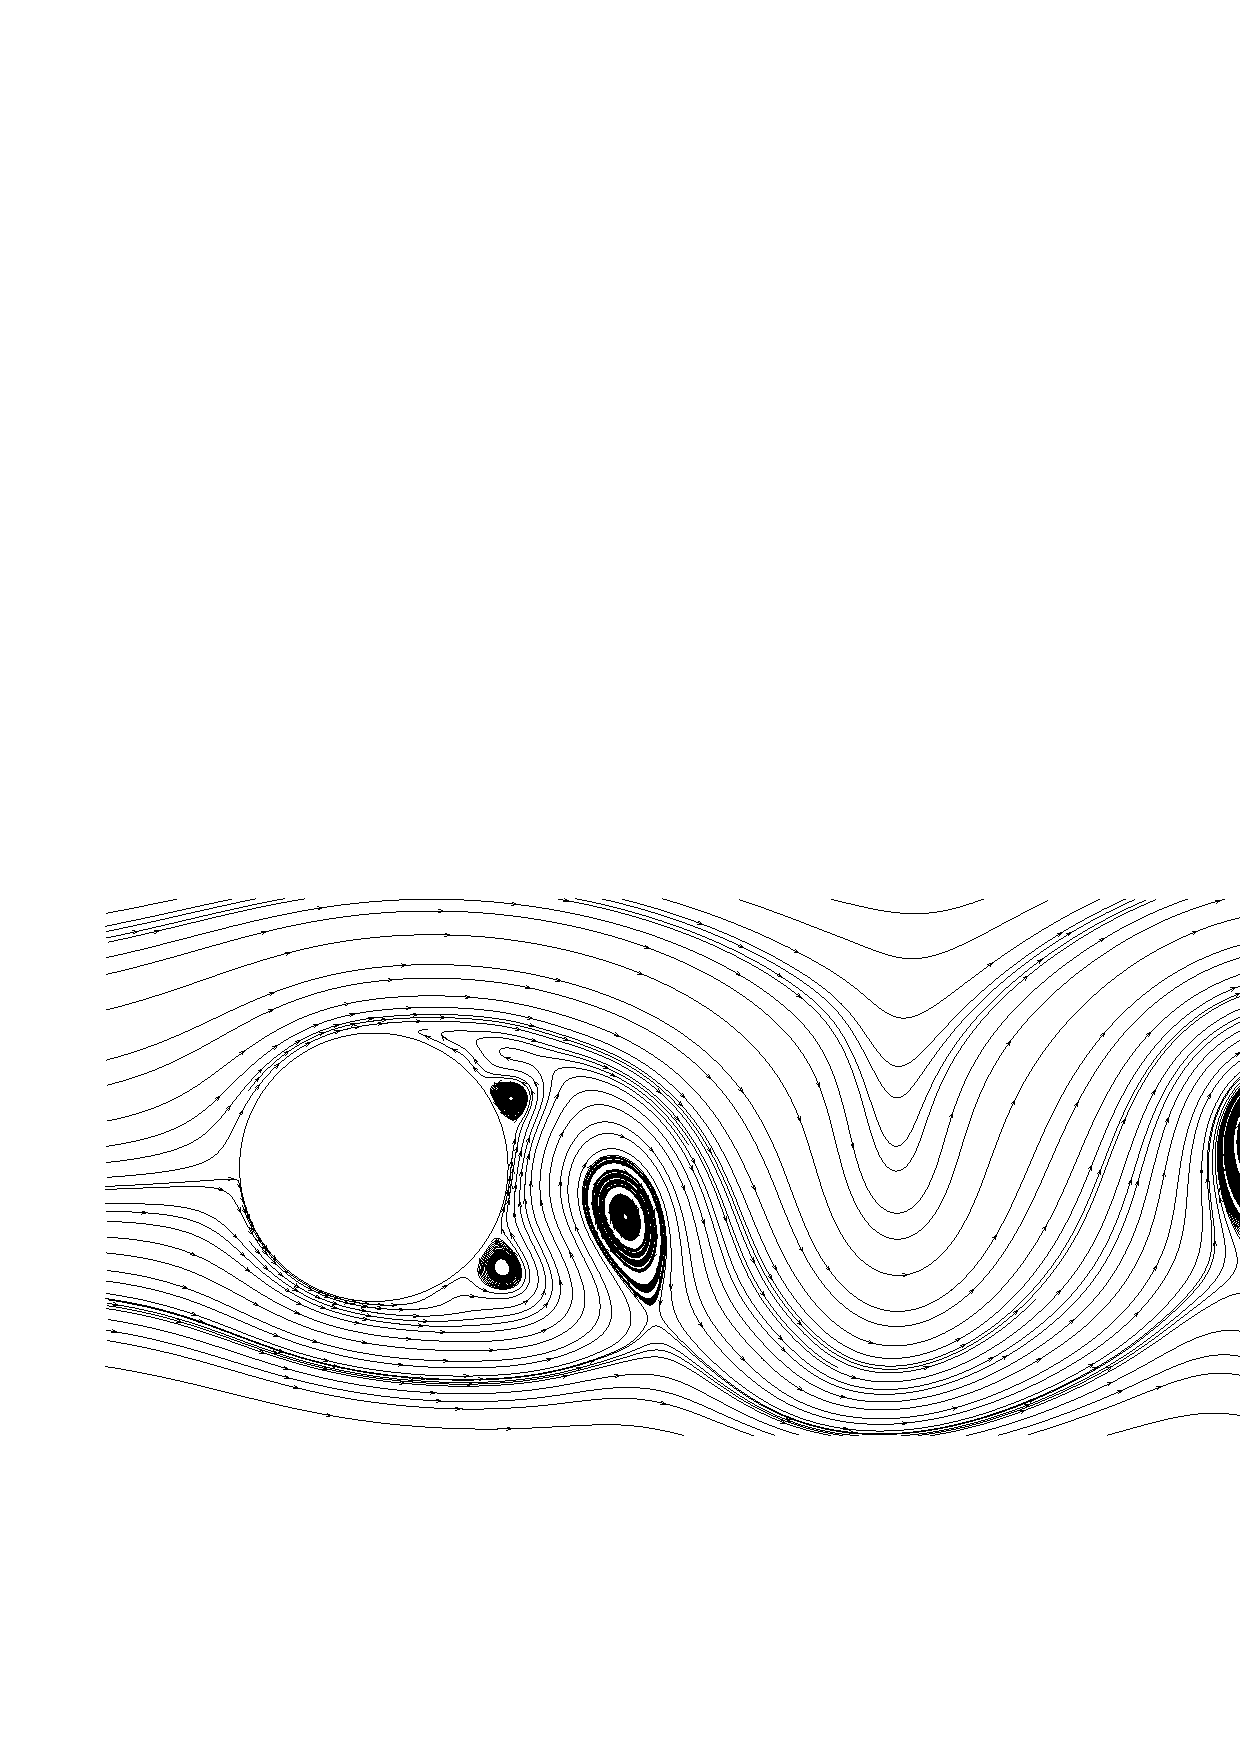
\includegraphics[width=45mm,clip=t]{CHAP_NONLIN/FIGURE/cim4.pdf}
        \\
         Time 1 & Time 2 & Time 3
        \\
         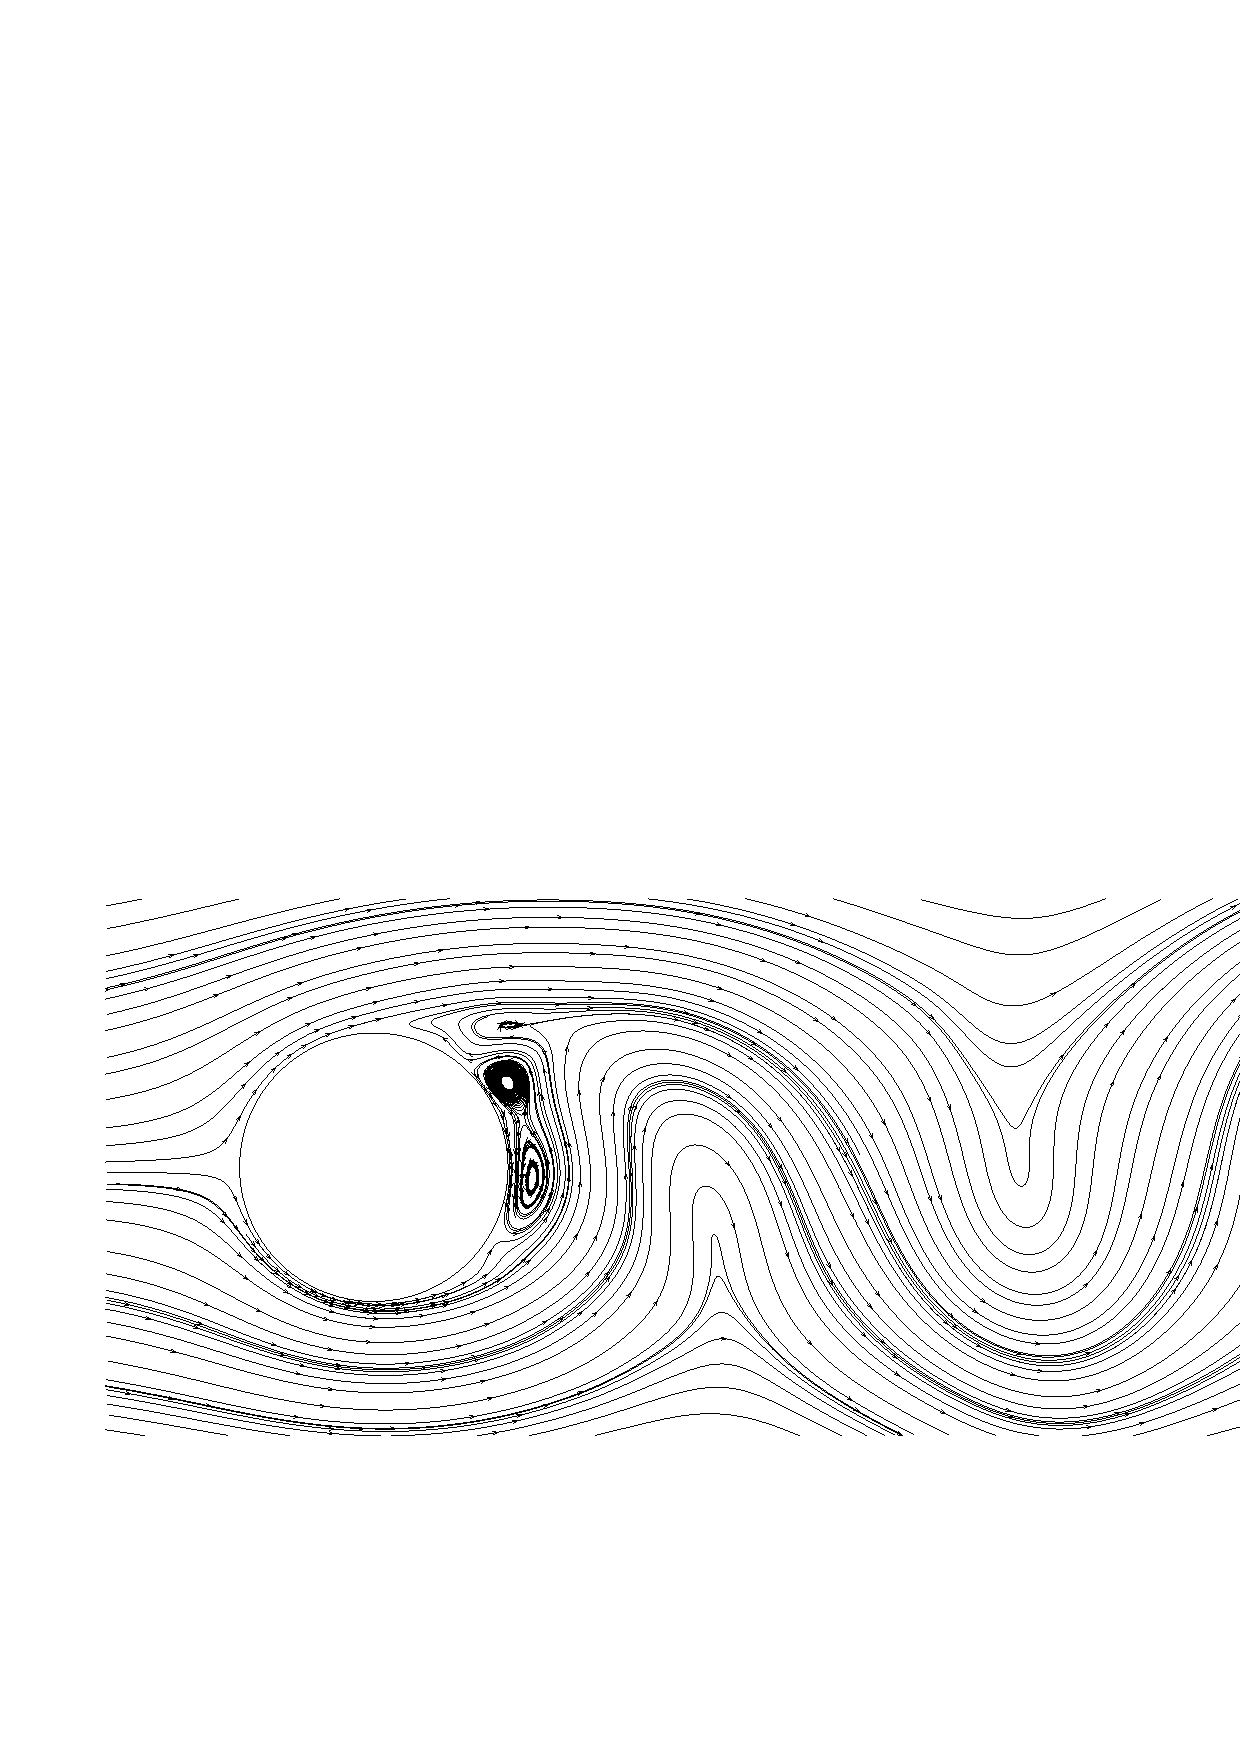
\includegraphics[width=45mm,clip=t]{CHAP_NONLIN/FIGURE/cim5.pdf}
         &
         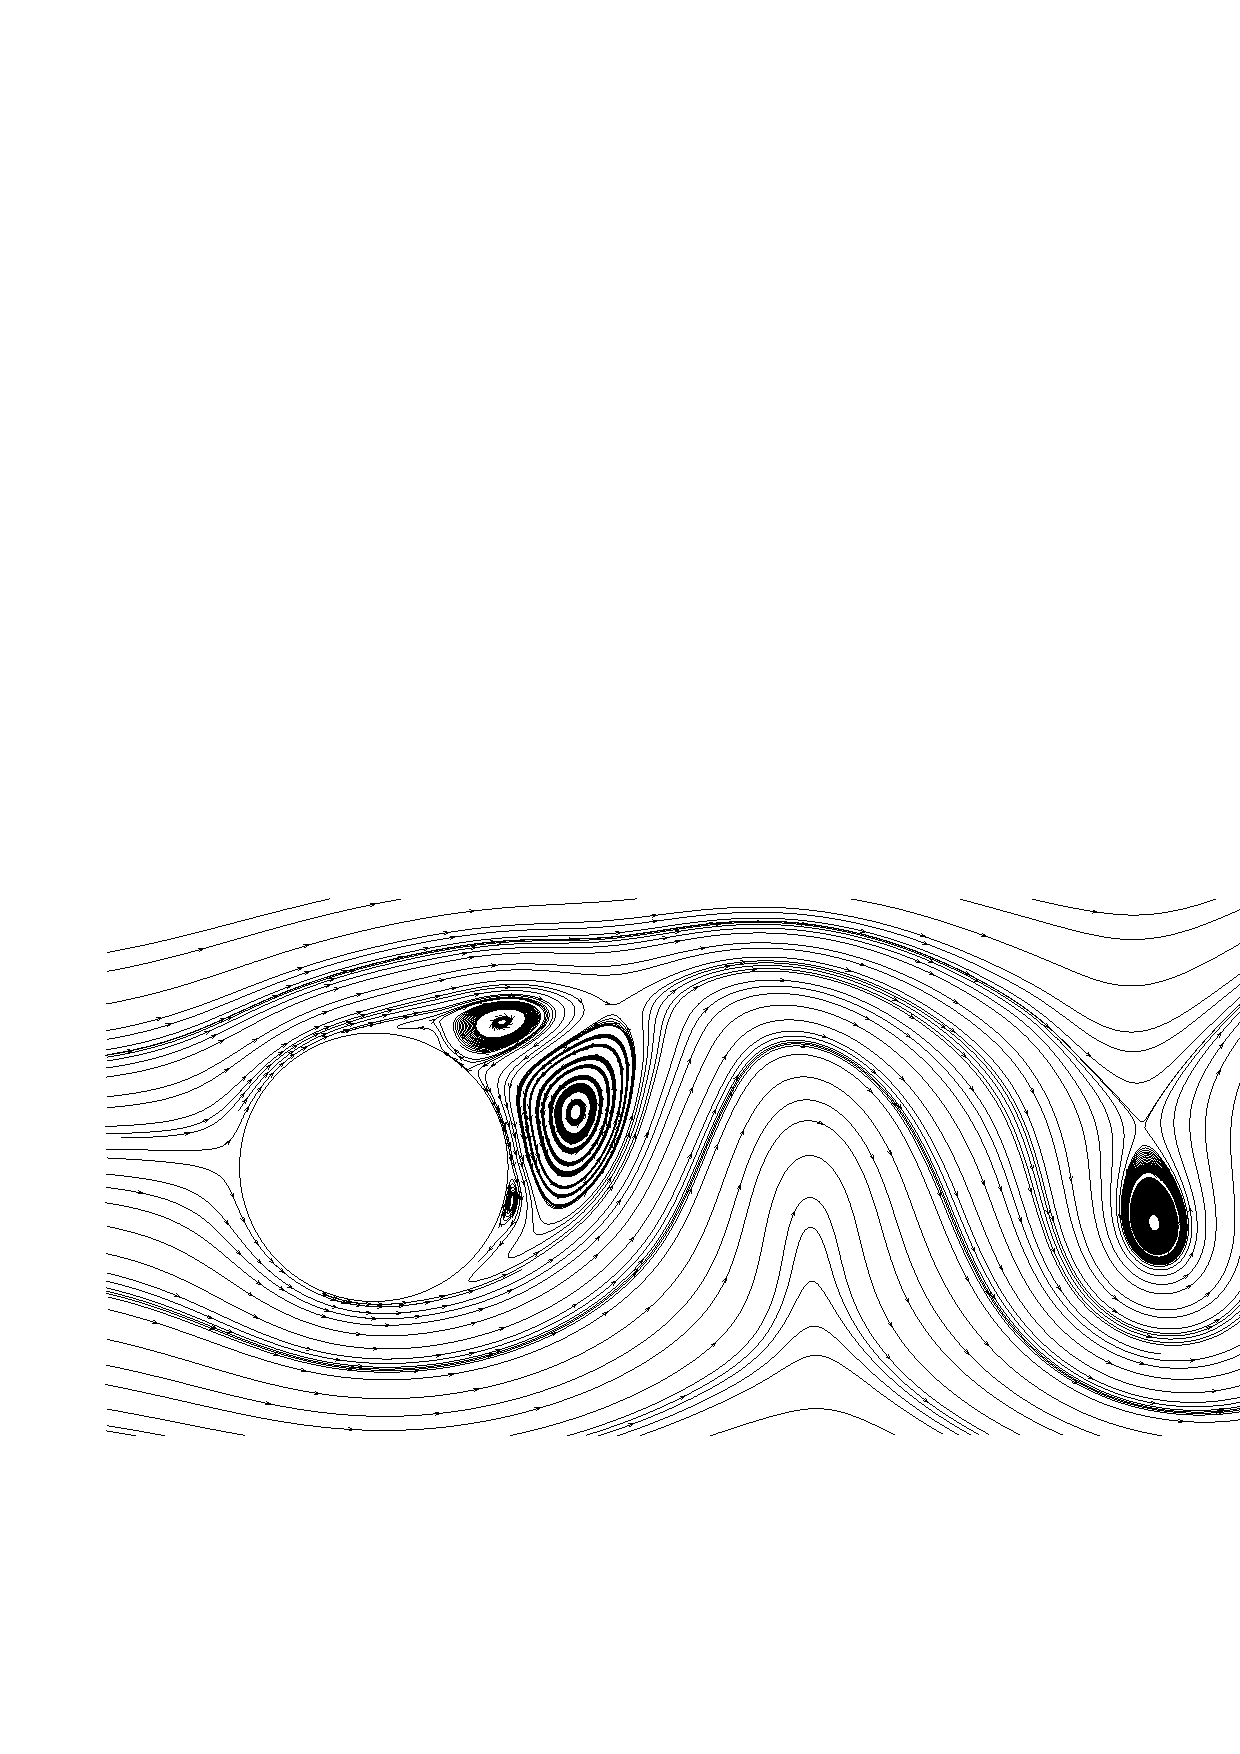
\includegraphics[width=45mm,clip=t]{CHAP_NONLIN/FIGURE/cim6.pdf}
         &
         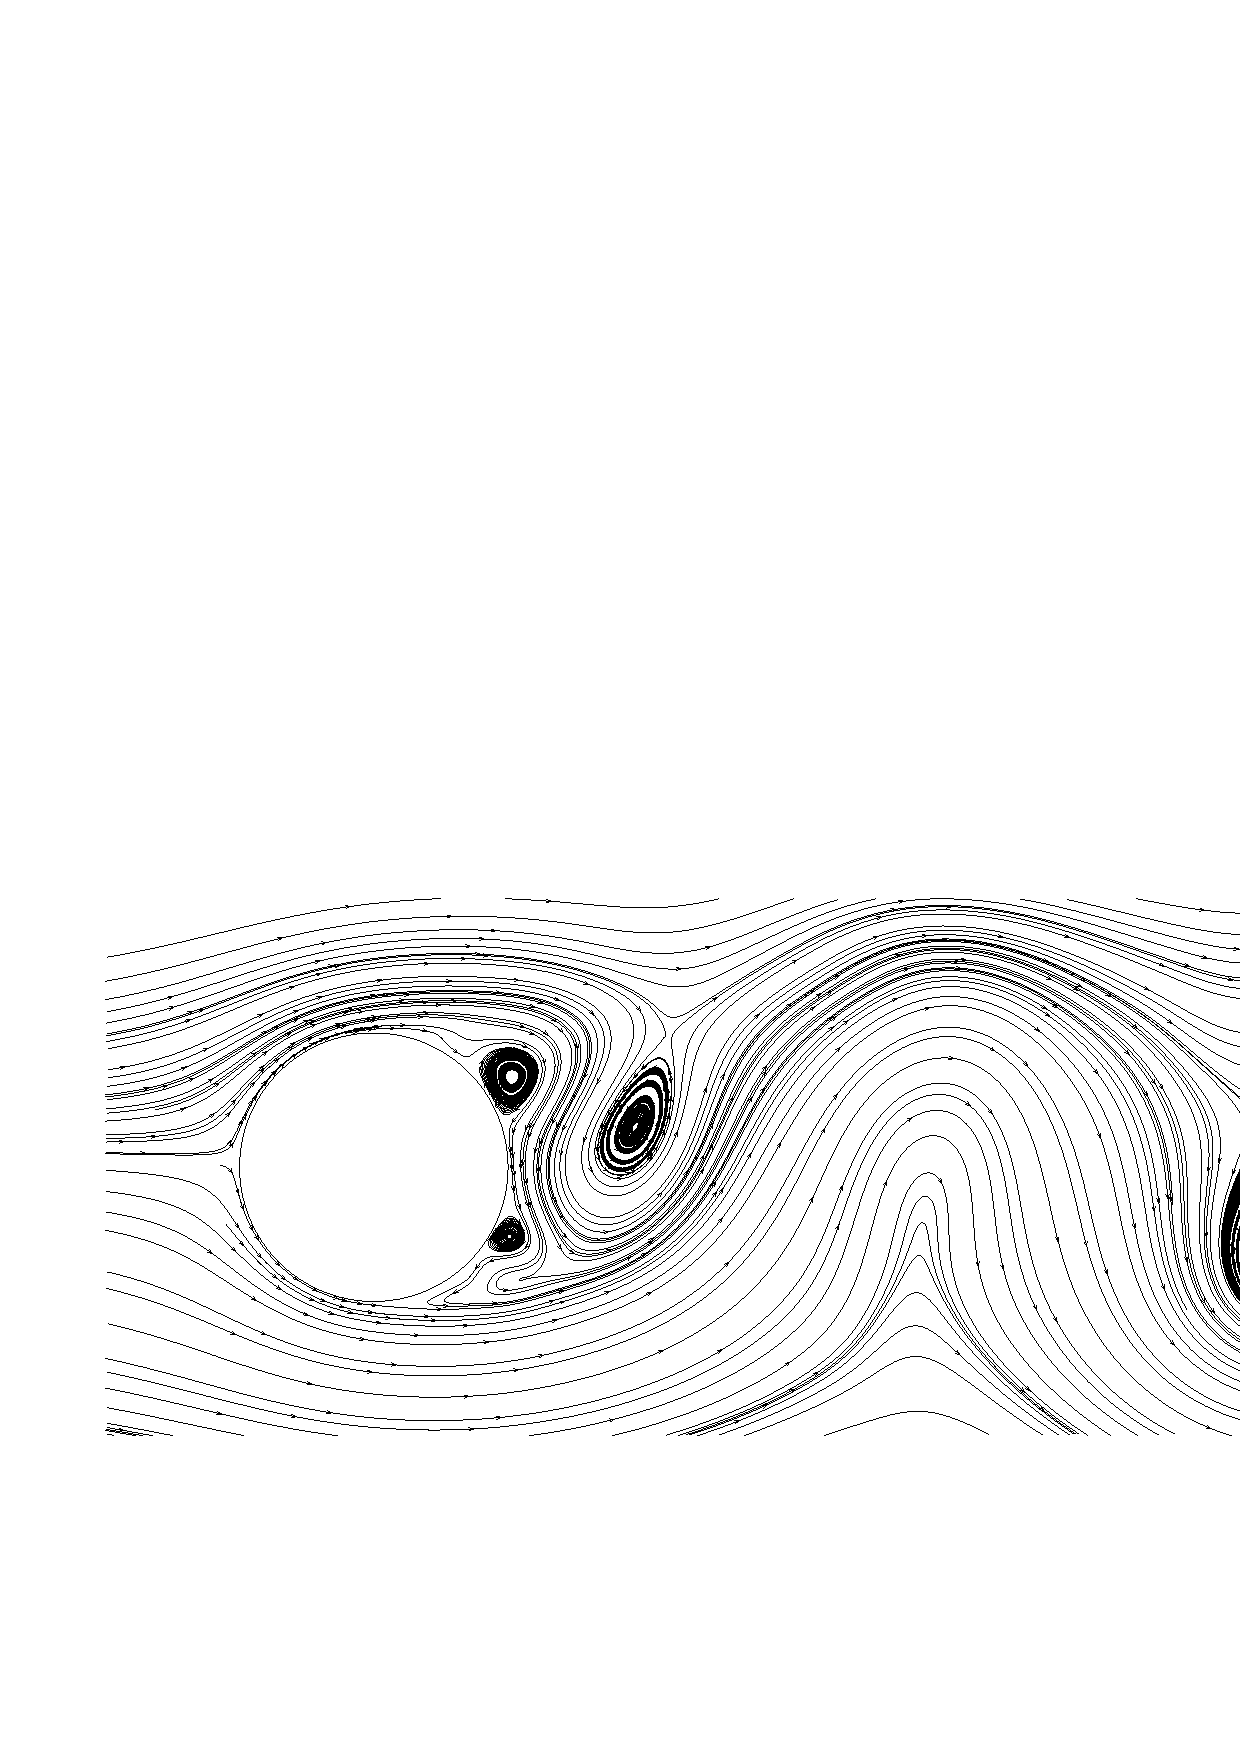
\includegraphics[width=45mm,clip=t]{CHAP_NONLIN/FIGURE/cim1.pdf}
        \\
         Time 4 & Time 5 & Time 6
       \end{tabular}}
  \end{tabular}
 \end{center}
 \vspace{-5mm}
 \caption{Circular cylinder. Instantaneous particle traces}
 \label{cil_sol1.fig}
\end{figure}
%

 Figs. \ref{cil_sol1.fig} reports the instantaneous
 particle traces in six instants over a cycle (the seventh position would be
 equivalent to the first) for two different $Re_d$.
 The shedding of the vortex is evident as well as the mechanism of their formation
 with a vortex merging. This is evident in Fig. \ref{cil_sol1.fig}a between instants
 3 and 4, and 6 and 1.
 It is worth to note the different pattern followed by the vortices for the two
 Reynolds number under consideration. For $Re_d= 400$ the
 shedding structure is well organised while for $Re_d= 4,000$
 the inertial forces play a more important role in the wake flow with formations
 of large recirculation bubbles which are propagated with small dissipation.
%

%
%
%
%
\subsection{Transonic buffeting over a bicircular airfoil}
\label{transonic_buffeting.subsec}
%
 Starting for about 1976, several experiments were
 carried out on transonic buffeting over bicircular-arc airfoils
 at NASA Ames research center with the intent to provide
 basic data to guide further development of computer codes
 (McDevitt et al. \citeyearNP{McDevitt:1}).
 The wind tunnel used for those experiments was designed for
 this purpose in order to minimize upper and lower wall
 interference effects. The tests were conducted at free-stream
 Reynolds numbers, based on airfoil chord length, ranging from 1
 to 17 million. The test Mach number was varied from near the critical
 value of 0.71 to the highest possible without the airfoil chocking
 the channel.
 McDevitt et al. \citeyear{McDevitt:1} presented unsteady results for
 a biconvex circular-arc airfoil with thickness-chord ratio of 0.18.
 The nominal test Mach for this airfoil is 0.775 and the wind
 tunnel end walls were designed to minimize wall effects for this flow
 condition.
%
%
\begin{figure}[ht]
 \begin{center}
  \begin{tabular}{ccc}
    \subfigure[Time 1]
       {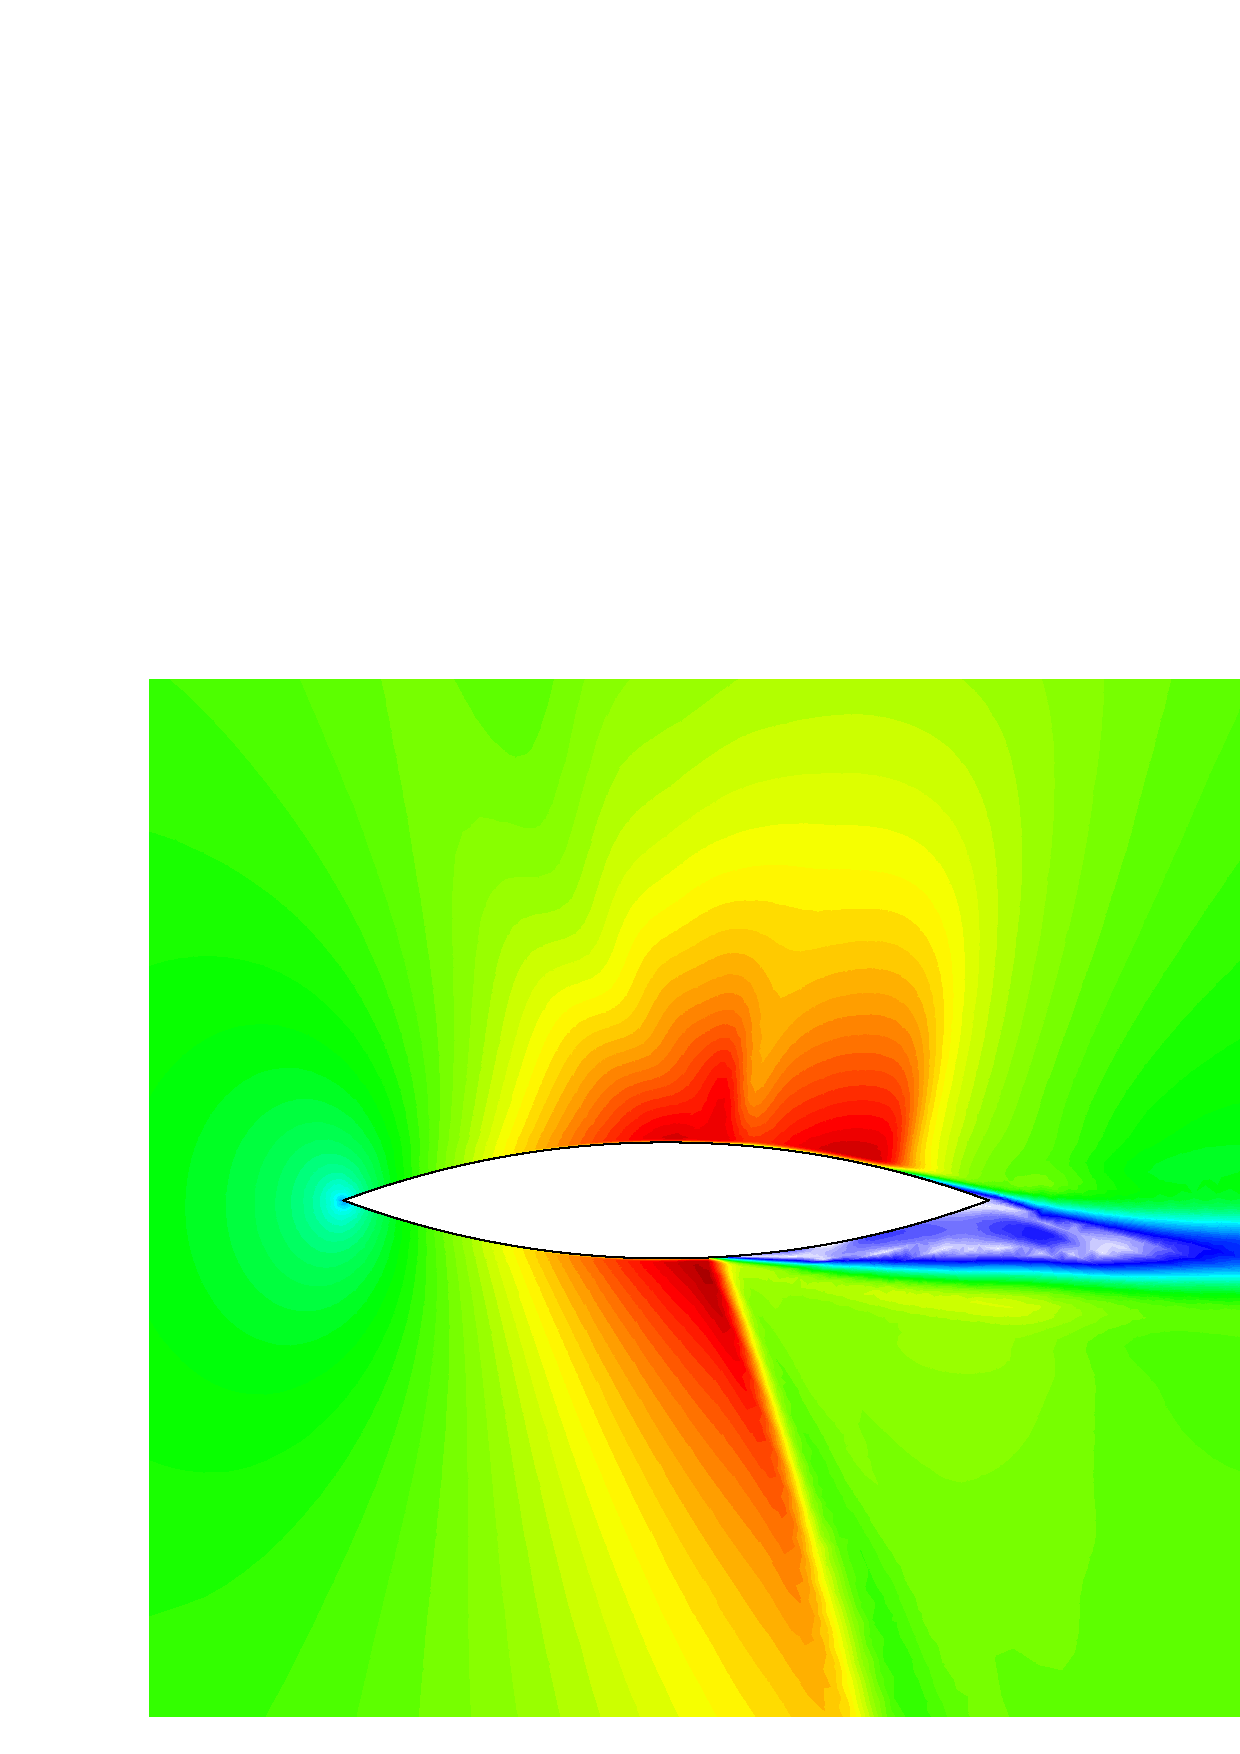
\includegraphics[width=45mm,clip=t]{CHAP_NONLIN/FIGURE/arc1.pdf}}
        &
    \subfigure[Time 2]
       {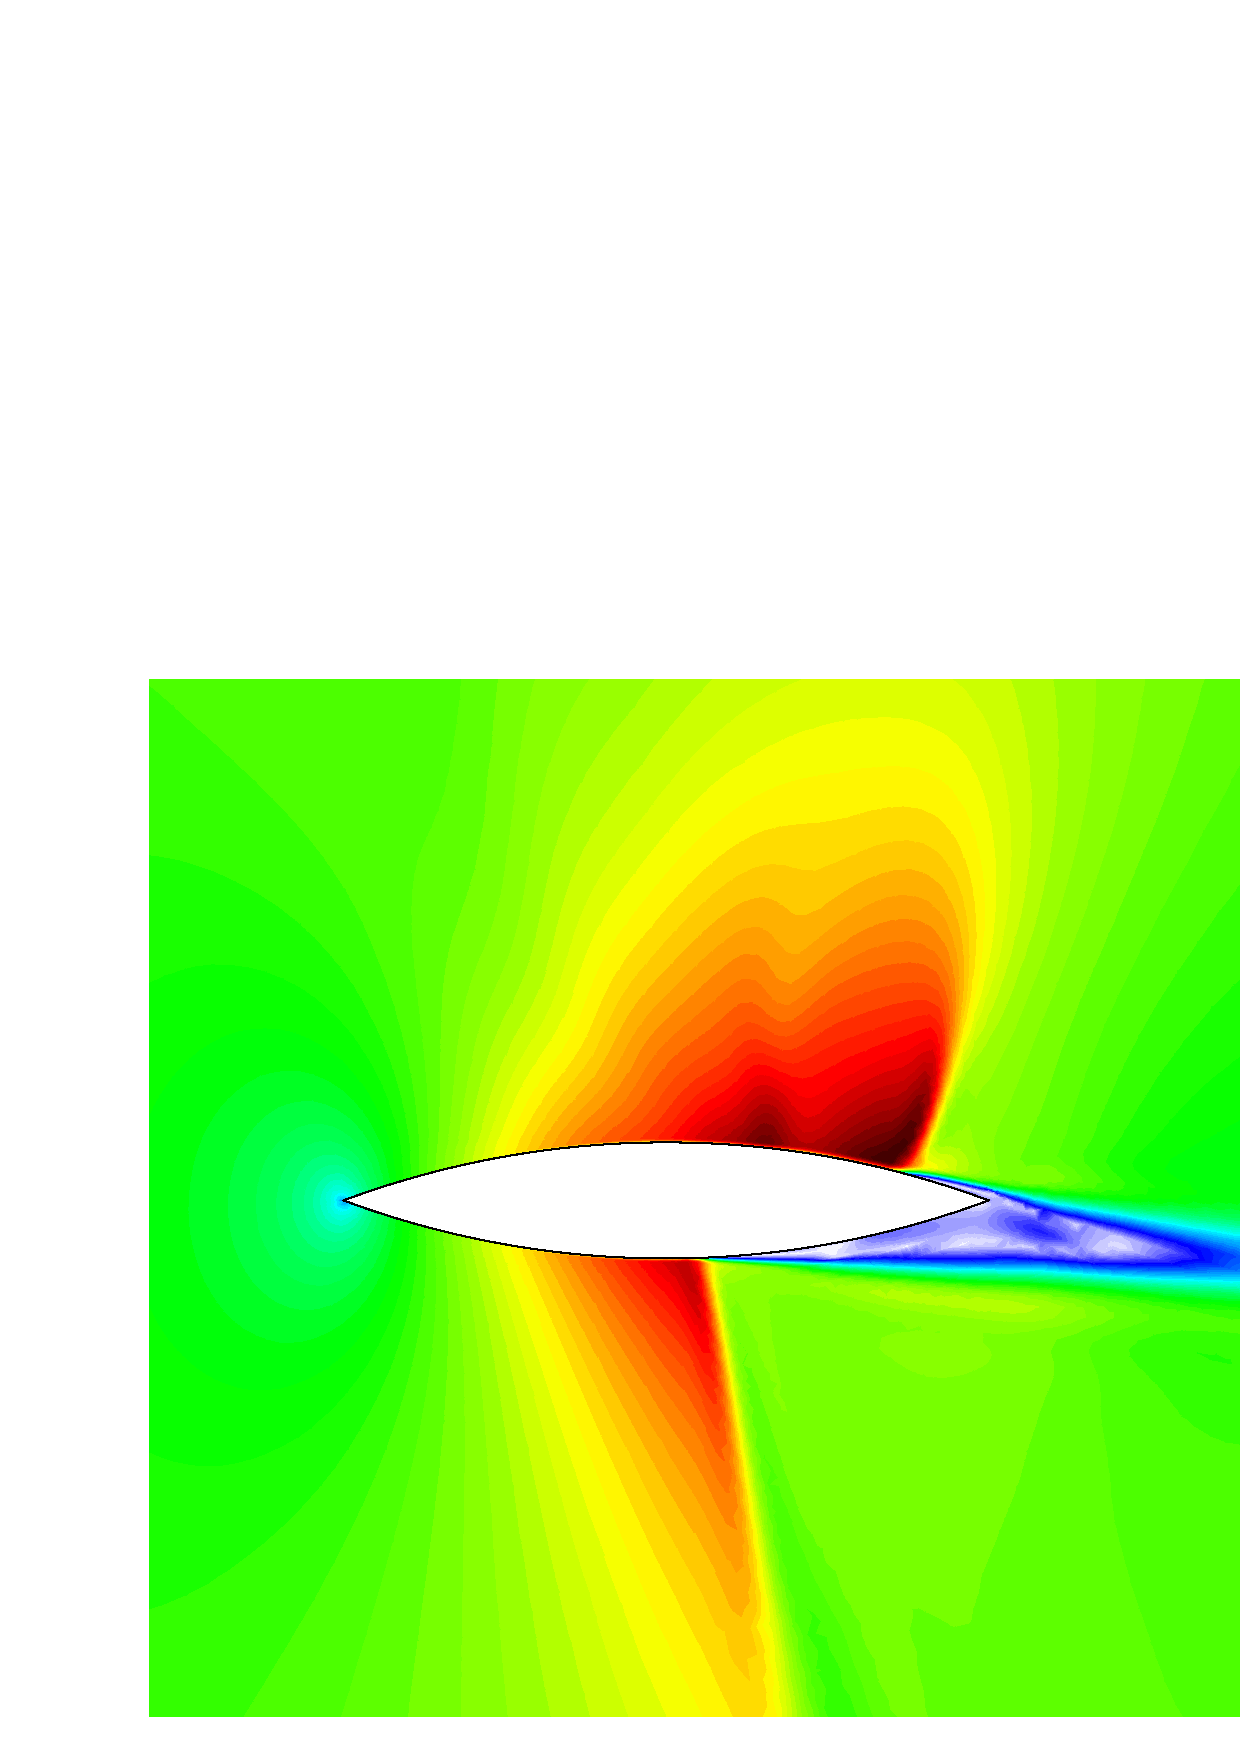
\includegraphics[width=45mm,clip=t]{CHAP_NONLIN/FIGURE/arc2.pdf}}
        &
    \subfigure[Time 3]
       {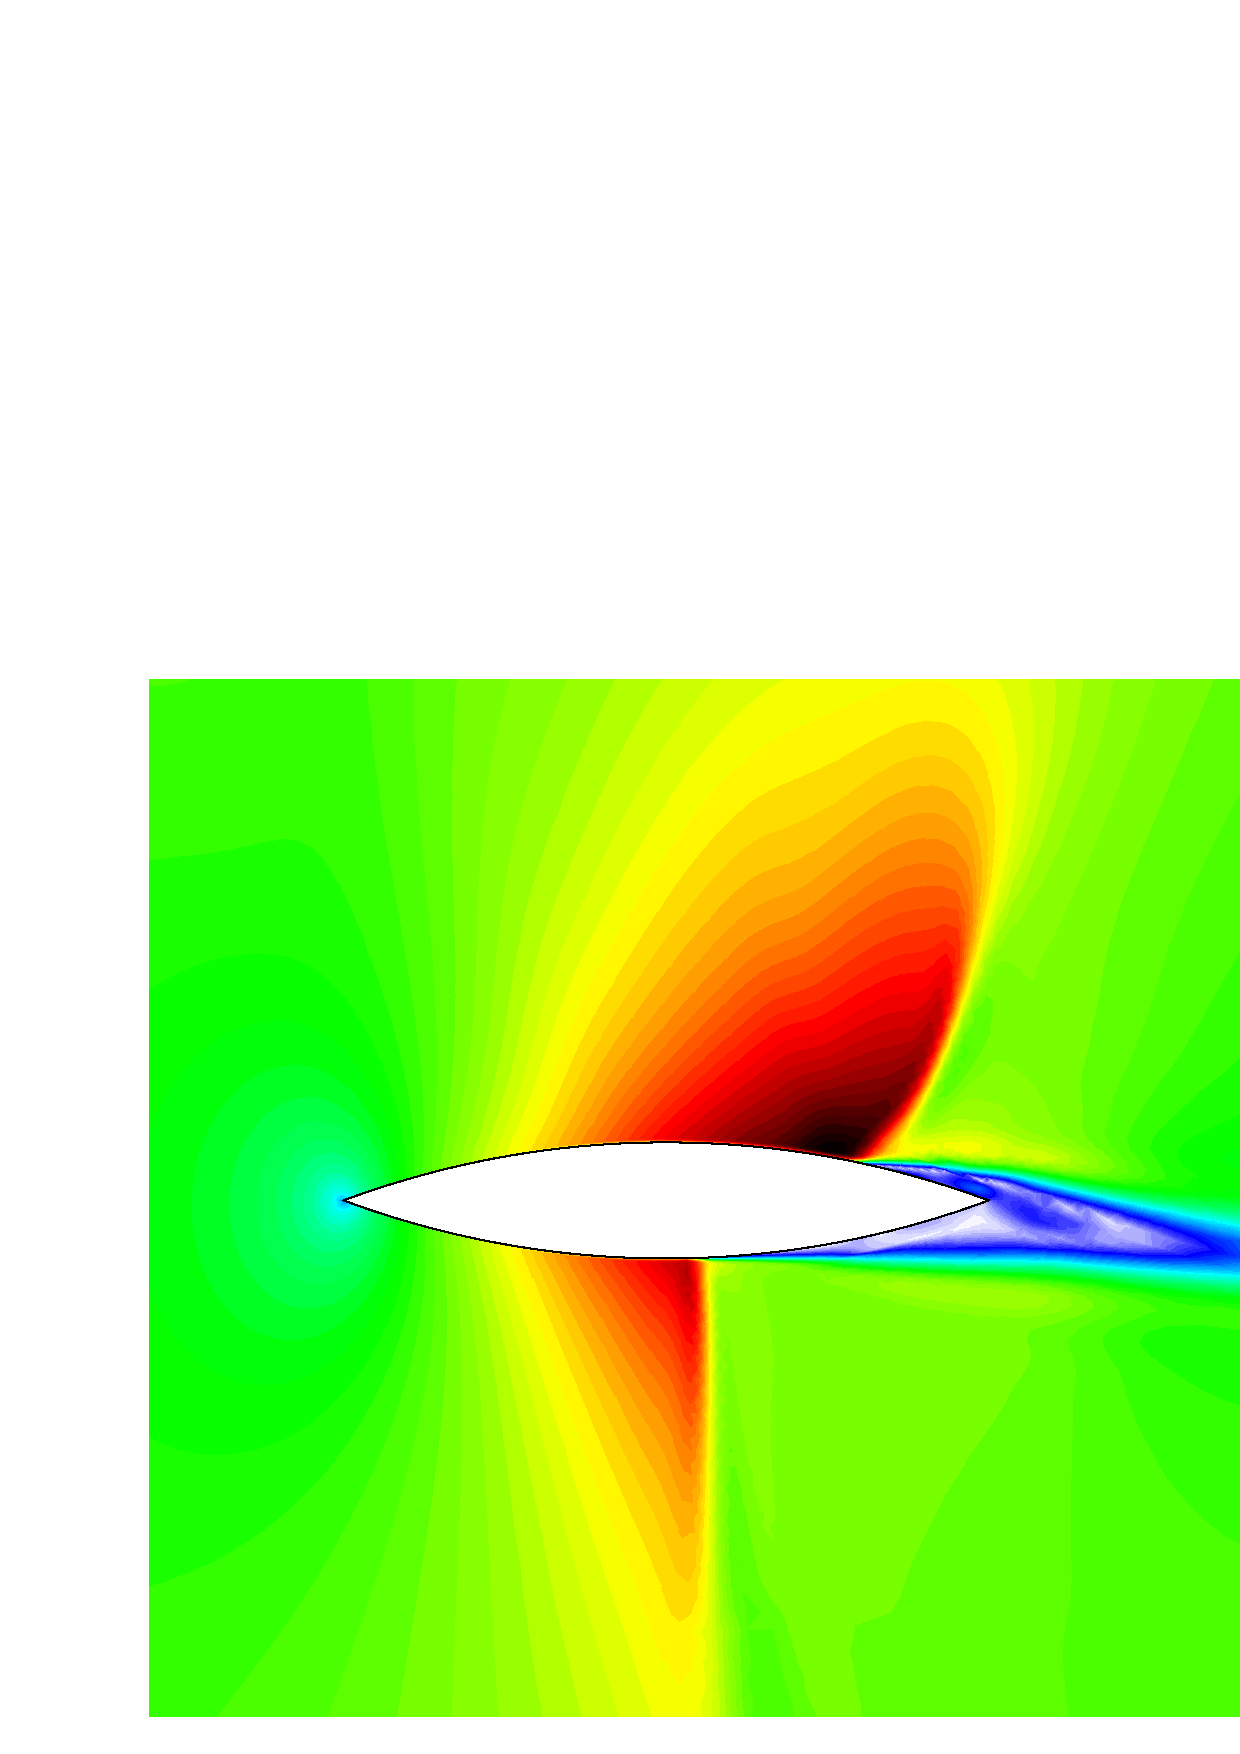
\includegraphics[width=45mm,clip=t]{CHAP_NONLIN/FIGURE/arc3.pdf}}
        \vspace{-4mm}\\
    \subfigure[Time 4]
       {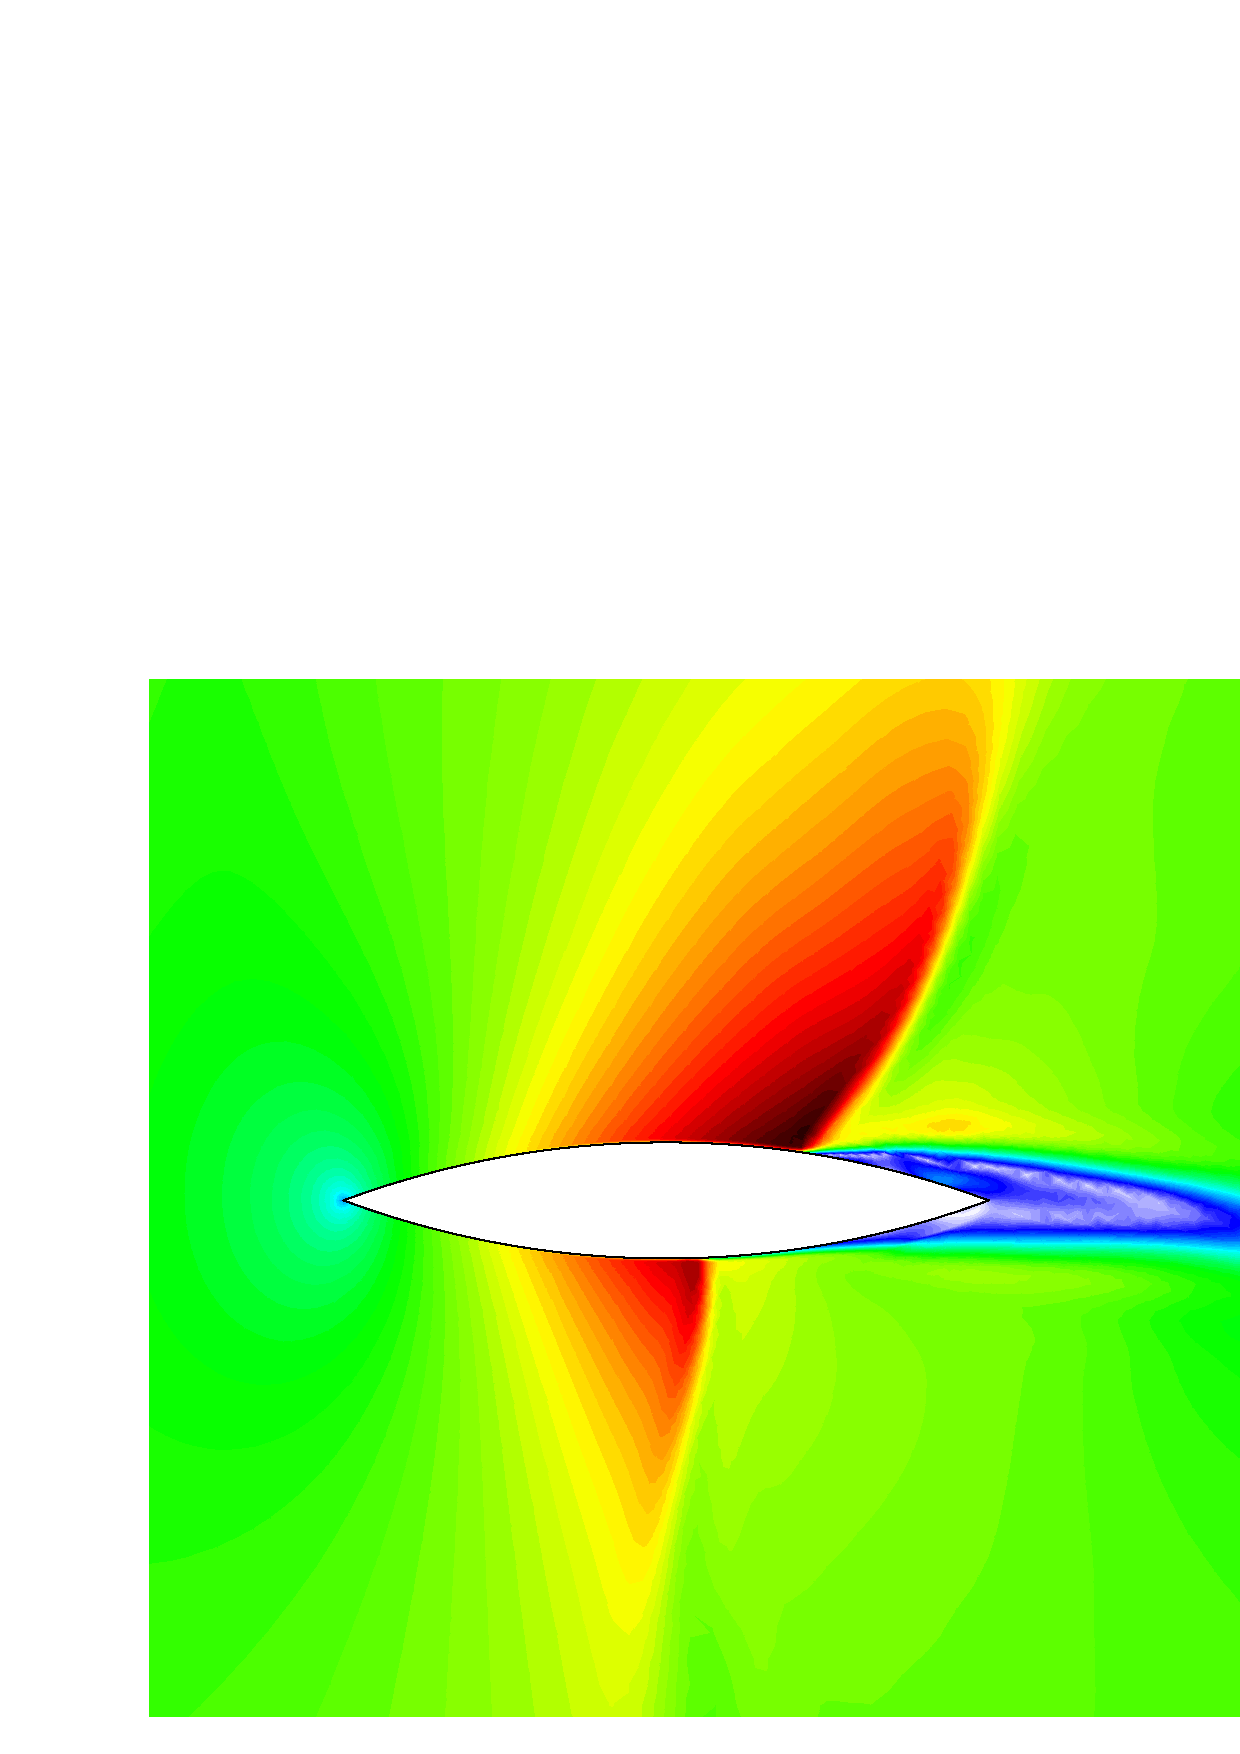
\includegraphics[width=45mm,clip=t]{CHAP_NONLIN/FIGURE/arc4.pdf}}
        &
    \subfigure[Time 5]
       {\includegraphics[width=45mm,clip=t]{CHAP_NONLIN/FIGURE/arc5.pdf}}
        &
    \subfigure[Time 6]
       {\includegraphics[width=45mm,clip=t]{CHAP_NONLIN/FIGURE/arc6.pdf}}
        \vspace{-4mm}\\
    \subfigure[Time 7]
       {\includegraphics[width=45mm,clip=t]{CHAP_NONLIN/FIGURE/arc7.pdf}}
        &
    \subfigure[Time 8]
       {\includegraphics[width=45mm,clip=t]{CHAP_NONLIN/FIGURE/arc8.pdf}}
        &
    \subfigure[Time 9]
       {\includegraphics[width=45mm,clip=t]{CHAP_NONLIN/FIGURE/arc9.pdf}}
        \vspace{-4mm}\\
    \subfigure[Time 10]
       {\includegraphics[width=45mm,clip=t]{CHAP_NONLIN/FIGURE/arc10.pdf}}
        &
    \subfigure[Time 11]
       {\includegraphics[width=45mm,clip=t]{CHAP_NONLIN/FIGURE/arc11.pdf}}
        &
    \subfigure
       {\includegraphics[width=45mm,clip=t]{CHAP_NONLIN/FIGURE/arc12.pdf}}
  \end{tabular}
 \end{center}
 \vspace{-5mm}
 \caption{Bicircular airfoil. $M_\infty = 0.775$,
          $Re_\infty = 7\cdot10\se{6}$. Instantaneous Mach number contours}
 \label{arc_sol1.fig}
\end{figure}
%
 At a free-stream Reynolds number of 7 million, experiments suggest
 transonic buffeting at a free stream Mach number in the range
 from 0.76 to 0.78. On the contrary, the calculations show
 unsteadiness in the Mach number range from 0.765 up to 0.83.
 The computed buffeting reduced frequency $\pi f c/u\sm{\infty}$
 matches the experimental one of $\approx 0.5$.

 Fig. \ref{arc_sol1.fig} reports instantaneous Mach number contours
 in eleven instants over a cycle while Fig. \ref{arc_sol2.fig}a
 shows the average and range of pressure coefficient distribution
 in the airfoil surface.
%
\begin{figure}
 \begin{center}
  \begin{tabular}{c}
    \subfigure[pressure coefficient distribution]
     {\includegraphics[height=90mm,clip=t]{CHAP_NONLIN/FIGURE/arc_uns.pdf}}
        \\
    \subfigure[pressure coefficient evolution]
     {\includegraphics[height=90mm,clip=t]{CHAP_NONLIN/FIGURE/arc_per.pdf}}
  \end{tabular}
 \end{center}
 \vspace{-5mm}
 \caption{Bicircular airfoil. Computed pressure coefficient}
 \label{arc_sol2.fig}
\end{figure}
%
 Fig. \ref{arc_sol2.fig}b reports the evolution in time of the pressure
 coefficient at a point in the airfoil corresponding to $x/c = 0.7$.
 The time history refers to three cycles of oscillation after a periodic
 flow  condition is reached. The calculations were performed
 using roughly 45 divisions over a cycle
 (as indicated in Fig. \ref{arc_sol2.fig}b). This correspond to a local CFL
 number between 0.1 in the far-field and 10,000 in the boundary layer.
%
%

%
%
\section{Concluding Remarks}
\headb{Nonlinear Navier-Stokes solver}{Concluding remarks}
%
\begin{itemize}
%
 \item
 A FV scheme for the solution of the Favre averaged
 Navier-Stokes equations has been presented. The method employs an edge-based
 data structure as well as  a nearest-neighbour stencil for the discretisation of
 the Laplacian operator. The method enables the use of 2D and 3D
 unstructured, structured or block structured mixed-element grids without any modifications
 to the numerical scheme.
% 
\item
 A drawback of this approach is the need to evaluate the mixed
 derivative terms of the viscous fluxes by using a standard FV method which does not yield
 a nearest neighbour stencil.
 However, in cases where the viscous effects are in the boundary layer
 only, such terms are
 very small and hence the method is expected to be well suited to
 engineering applications.
%
\item
 The same time relaxation multigrid algorithm has been applied to both
 steady and unsteady time-marching aerodynamics. The benefit of unconditional
 stability has been demonstrated by computing unsteady
 viscous flow with time-steps corresponding to CFL numbers on the
 range 1000 - 10,000.
%
\item
 The multigrid technique efficiently performs for steady-state flow
 computations even though its robustness needs to be improved for 3D
 turbulent flow simulations.
 For time-marching unsteady flows, the multigrid technique does not
 perform as well. Convergence histories similar to the one
 shown in Fig. \ref{flat_impul.fig}b represents the best result
 obtained. The reason for such a break down is not clear. However
 the stability restriction in (\ref{local_time_step_2.eq}) could
 play and important part near the far-field boundaries.
%
\item
 For unsteady computations, an attractive way forward could be the
 implementation of an adaptive scheme which select different
 time-marching techniques in different zones depending on the
 local situation.
%
\item
 The scheme produces good and stable results for highly distorted
 meshes as demonstrated by Sbardella \& Imregun \citeyear{Luca:11}. 
%
\end{itemize}
%
